% !TEX program = pdflatex
% CableTract --- Prototype-Free Feasibility Study
% Compile: pdflatex cabletract_manuscript.tex (twice for cross-refs)

\documentclass[11pt,a4paper]{article}

% --------------------------------------------------------------------
% Packages
% --------------------------------------------------------------------
\usepackage[utf8]{inputenc}
\usepackage[T1]{fontenc}
\usepackage{lmodern}
\usepackage[english]{babel}
\usepackage[a4paper,margin=2.4cm]{geometry}
\usepackage{microtype}
\usepackage{amsmath,amssymb,amsthm}
\usepackage{mathtools}
\usepackage{siunitx}
\usepackage{graphicx}
\usepackage{float}
\usepackage{booktabs}
\usepackage{longtable}
\usepackage{array}
\usepackage{multirow}
\usepackage{tabularx}
\usepackage{caption}
\usepackage{subcaption}
\usepackage{xcolor}
\usepackage{enumitem}
\usepackage{tikz}
\usetikzlibrary{positioning,calc,arrows.meta,decorations.pathreplacing,backgrounds,shapes.geometric,fit,patterns}
\usepackage[hidelinks,colorlinks=true,linkcolor=blue!60!black,citecolor=blue!60!black,urlcolor=blue!60!black]{hyperref}
\usepackage[nameinlink,capitalise]{cleveref}
\usepackage[acronym,nonumberlist,nopostdot,toc]{glossaries}

\graphicspath{{figures/}}

% siunitx setup
\sisetup{
    detect-all,
    per-mode = symbol,
    range-phrase = --,
    range-units = single,
    group-separator = {\,},
    group-minimum-digits = 4
}
\DeclareSIUnit{\decare}{decare}
\DeclareSIUnit{\hectare}{ha}
\DeclareSIUnit{\litre}{L}
\DeclareSIUnit{\year}{yr}
\DeclareSIUnit{\Wh}{Wh}
\DeclareSIUnit{\kWh}{kWh}
\DeclareSIUnit{\auger}{augers}
\DeclareSIUnit{\EUR}{EUR}
\DeclareSIUnit{\USD}{USD}
\DeclareSIUnit{\hp}{hp}

% Repository for the analytical implementation
\newcommand{\cabletractrepo}{\url{https://github.com/yilmazozgur/cabletract}}

% Caption style
\captionsetup{font=small,labelfont=bf,format=plain,justification=raggedright,singlelinecheck=false}

% Tighter table notes
\newcommand{\tabnote}[1]{{\footnotesize\textit{Note.} #1}}

% Section spacing
\usepackage{titlesec}
\titleformat{\section}{\normalfont\Large\bfseries}{\thesection}{0.6em}{}
\titleformat{\subsection}{\normalfont\large\bfseries}{\thesubsection}{0.6em}{}
\titleformat{\subsubsection}{\normalfont\normalsize\bfseries}{\thesubsubsection}{0.6em}{}
\titlespacing*{\section}{0pt}{1.4ex}{0.7ex}
\titlespacing*{\subsection}{0pt}{1.1ex}{0.5ex}
\titlespacing*{\subsubsection}{0pt}{0.9ex}{0.4ex}

% --------------------------------------------------------------------
% Acronym glossary --- every acronym used in the paper, defined here
% so the first use in the body expands automatically via \gls{}.
% --------------------------------------------------------------------
\makeglossaries

% Domain & standards
\newacronym{asabe}{ASABE}{American Society of Agricultural and Biological Engineers}
\newacronym{iwrc}{IWRC}{Independent Wire Rope Core}
\newacronym{ice}{ICE}{Internal Combustion Engine}
\newacronym{ice3}{ICE\,v3}{Inventory of Carbon and Energy, version 3 (Hammond \& Jones)}
\newacronym{ev}{EV}{Electric Vehicle}
\newacronym{wd}{4WD}{Four-Wheel Drive}
\newacronym{lca}{LCA}{Life-Cycle Assessment}
\newacronym{lcoe}{LCOE}{Levelised Cost of Energy / Operation}
\newacronym{npv}{NPV}{Net Present Value}
\newacronym{dcf}{DCF}{Discounted Cash Flow}
\newacronym{capex}{CAPEX}{Capital Expenditure}
\newacronym{opex}{OPEX}{Operating Expenditure}
\newacronym{bom}{BoM}{Bill of Materials}
\newacronym{bos}{BoS}{Balance of System (PV cabling, mounting, inverter)}
\newacronym{eu}{EU}{European Union}
\newacronym{latam}{LATAM}{Latin America}

% Powertrain & hardware
\newacronym{pmsm}{PMSM}{Permanent-Magnet Synchronous Motor}
\newacronym{bldc}{BLDC}{Brushless DC motor}
\newacronym{pv}{PV}{Photovoltaic}
\newacronym{vawt}{VAWT}{Vertical-Axis Wind Turbine}
\newacronym{soc}{SoC}{State of Charge}
\newacronym{bms}{BMS}{Battery Management System}
\newacronym{gnss}{GNSS}{Global Navigation Satellite System}
\newacronym{gps}{GPS}{Global Positioning System}

% Energy / weather data sources
\newacronym{tmy}{TMY}{Typical Meteorological Year}
\newacronym{ghi}{GHI}{Global Horizontal Irradiance}
\newacronym{doy}{DOY}{Day Of Year}
\newacronym{nrel}{NREL}{(US) National Renewable Energy Laboratory}
\newacronym{nsrdb}{NSRDB}{(NREL) National Solar Radiation Database}
\newacronym{pvgis}{PVGIS}{(EU JRC) Photovoltaic Geographical Information System}
\newacronym{sarah}{SARAH2}{Surface Solar Radiation Data Set --- Heliosat, version 2}
\newacronym{niwe}{NIWE}{(India) National Institute of Wind Energy}
\newacronym{inmet}{INMET}{(Brazil) National Institute of Meteorology}
\newacronym{swera}{SWERA}{Solar and Wind Energy Resource Assessment}

% Statistical & ML
\newacronym{p10}{P10}{10th percentile of a sampled distribution}
\newacronym{p50}{P50}{50th (median) percentile of a sampled distribution}
\newacronym{p90}{P90}{90th percentile of a sampled distribution}
\newacronym{gbt}{GBT}{Gradient-Boosted Trees (regression)}
\newacronym{gbr}{GBR}{Gradient Boosting Regressor (scikit-learn)}
\newacronym{nsga}{NSGA-II}{Non-dominated Sorting Genetic Algorithm, version II}
\newacronym{salib}{SALib}{Sensitivity Analysis Library (Python)}
\newacronym{sobol1}{S1}{Sobol first-order sensitivity index}
\newacronym{sobolt}{ST}{Sobol total-order sensitivity index}
\newacronym{rmse}{RMSE}{Root Mean Squared Error}
\newacronym{r2}{R\textsuperscript{2}}{Coefficient of determination}

% Data, agencies, methods
\newacronym{fem}{FEM}{Finite Element Method}
\newacronym{usda}{USDA NASS}{(US) Department of Agriculture, National Agricultural Statistics Service}
\newacronym{defra}{DEFRA}{(UK) Department for Environment, Food \& Rural Affairs}
\newacronym{eea}{EEA}{European Environment Agency}
\newacronym{ivl}{IVL}{IVL Swedish Environmental Research Institute}
\newacronym{inrae}{INRAE}{French National Research Institute for Agriculture, Food and Environment}
\newacronym{dlg}{DLG}{Deutsche Landwirtschafts-Gesellschaft}
\newacronym{bnef}{BloombergNEF}{Bloomberg New Energy Finance}
\newacronym{api}{API}{Application Programming Interface}

% Concepts unique to this paper
\newacronym{mu}{MU}{Main Unit (winch + motor + battery + harvester module)}
\newacronym{rq}{RQ}{Research Question}
\newacronym{c1}{C1}{compaction-reduction claim}
\newacronym{c2}{C2}{energy-reduction claim}
\newacronym{c3}{C3}{off-grid-feasibility claim}
\newacronym{c4}{C4}{economics and life-cycle CO\textsubscript{2} claim}

% --------------------------------------------------------------------
% Title block
% --------------------------------------------------------------------
\title{\textbf{CableTract: A Co-Designed Cable-Driven Field Robot for\\
Low-Compaction, Off-Grid Capable Agriculture}\\[0.4em]
\large A Prototype-Free Feasibility Study}
\author{Özgür Yılmaz\\[0.3em]
\normalsize Adana Science and Technology University, Adana, Türkiye\\[0.15em]
\normalsize \texttt{ozguryilmaz@atu.edu.tr} \quad \texttt{yilmazozgur.kaan@gmail.com}}
\date{April 2026}

% Glossary section heading customisation
\renewcommand{\acronymname}{List of acronyms}

\begin{document}
\maketitle

\begin{abstract}
\noindent
Conventional field operations spend most of their energy moving the tractor body, not the implement. Yet feasibility studies for novel agricultural vehicles rarely tie mechanics, energy harvest, draft, field geometry, economics, life-cycle CO\textsubscript{2}, and uncertainty quantification together on a single reproducible code path.

This paper builds such a framework and applies it to \textbf{CableTract}, a two-module cable-driven field robot. A stationary \gls{mu} (winch, motor, battery, solar and wind harvester) and a lighter Anchor module (held by helical screw piles) tension a cable across a strip while a lightweight implement carriage rolls along it. The heavy bodies stay on the headland; only the carriage enters the field.

The carriage runs a 10-implement library \emph{co-designed for the cable architecture}: narrower (\SI{1.5}{\meter} vs.\ \SI{3}{\meter}), shallower (${\sim}\,0.85\times$ depth), slower (\SIrange{1}{2.5}{\kilo\meter\per\hour} vs.\ \SIrange{5}{9}{\kilo\meter\per\hour}), and lighter than implements borrowed from conventional tractor inventories. This co-design is the paper's central analytical lever.

\medskip
The framework is prototype-free. It chains a catenary cable model, a drivetrain efficiency chain, a stochastic draft model fitted to the co-designed library, an hourly solar\,+\,wind\,+\,battery simulator on six sites, a polygon coverage planner on a 50-field corpus, a contact-pressure compaction model, a discounted-cash-flow economics engine with battery replacement and life-cycle CO\textsubscript{2}, and a global sensitivity analysis on 20 inputs. An operating-envelope sweep and an architectural-variant comparison close the loop. The full implementation is open source.\footnote{\cabletractrepo}

\medskip
Applied to the codesigned reference, the framework yields:
\begin{itemize}[leftmargin=1.4em,itemsep=0.15em]
    \item \textbf{Energy:} \SI{921}{\Wh\per\decare} (\SI{9.21}{\kWh\per\hectare}) --- roughly $18\times$ lower than the \SI{168}{\kWh\per\hectare} of an \SI{80}{hp} diesel tractor on the same operations.
    \item \textbf{Compaction:} ${\sim}98\%$ reduction in compacted \emph{area} and ${\sim}73\times$ reduction in the contact-energy index per cropping season, because only the \SI{250}{\kilogram} carriage rolls inside the field.
    \item \textbf{Off-grid:} \SI{13.8}{decares\per day} median throughput on harvested energy alone at Konya (\SI{15}{\meter\squared} \gls{pv} + \SI{9}{\kWh} battery); off-grid is achievable in solar-rich climates (Konya, Ludhiana, São Paulo), conditional in Mediterranean ones (Palencia, Des Moines), and not achievable at any practical hardware scale in northern temperate climates (Beauce).
    \item \textbf{Economics:} \gls{npv} versus diesel of \SI{+3978}{\EUR} at \SI{25}{\hectare\per\year} and 8\,\% discount, with discounted payback of \textbf{\SI{0.82}{\year}}. \gls{npv} is positive across the full \SIrange{1}{100}{\hectare\per\year} sweep at all three discount rates we test (5/8/12\,\%).
    \item \textbf{Life-cycle CO\textsubscript{2}:} \SI{14.6}{\kilogram\per\hectare\per\year} CO\textsubscript{2}eq versus 32.5 for the diesel reference and 22.9 for a Monarch-class electric tractor --- a clean $2.2\times$ improvement that does not depend on grid decarbonisation.
    \item \textbf{Operating envelope:} \gls{npv}-positive in 100\,\% of the 3\,600 cells of an (annual \gls{ghi} $\times$ farm size) sweep covering 800--\SI{2300}{\kWh\per\meter\squared\per\year} and \SIrange{1}{1000}{\hectare\per\year}, with discounted payback never exceeding \SI{1.85}{\year}. The binding constraint is off-grid feasibility at the upper-right corner (large farm, low \gls{ghi}), not financial viability.
\end{itemize}

\medskip
These numbers describe an \emph{internally consistent analytical envelope}, not a guarantee. The framework does not simulate closed-loop cable depth control, does not capture helical-pile retraction wear under repeated cycling, and does not model the Anchor's progressive self-disturbance of its own anchoring soil. \Cref{sec:open-risks} enumerates these open mechanical risks explicitly and identifies them --- not the financial or environmental claims --- as the dominant near-term feasibility question for the architecture. The contribution is therefore best read as a defensible analytical envelope and a reusable feasibility-analysis framework for similar studies, not as a finished system. We name the regime in which CableTract is internally consistent (medium-load operations on the co-designed library, $\geq\!10$ ha annual area, solar-rich climates) and identify the binding analytical constraints elsewhere (anchor reaction at heavy primary tillage, off-grid harvest in cloudy continental winters, polygon-shape losses on small fragmented fields).

\medskip
\noindent\textbf{Keywords:} feasibility framework, cable-driven agriculture, field robot, co-design, soil compaction, agricultural electrification, off-grid feasibility, NPV, life-cycle CO\textsubscript{2}, Sobol sensitivity analysis.
\end{abstract}

\tableofcontents

% ====================================================================
\section{Introduction}\label{sec:intro}
% ====================================================================

A modern \SI{80}{hp} \gls{wd} utility tractor weighs ${\approx}\SI{4}{\tonne}$, of which the implement is typically \SIrange{200}{500}{\kilogram}. Each pass therefore drags ten to twenty times more body mass than tool mass across the field, paying a soil-compaction penalty (mean contact pressure \SIrange{100}{250}{\kilo\pascal}, well above the \SI{50}{\kilo\pascal} threshold for clay soils) and burning ${\approx}\SI{12}{\litre\per\hectare}$ of diesel even on light operations. Over a 15-year lifetime on a \SI{25}{\hectare} farm this is \SI{4500}{\litre} of diesel and ${\approx}\SI{12}{\tonne}$ CO\textsubscript{2}eq.

CableTract attacks the dead-weight problem at the \emph{architectural} level rather than the powertrain level. Two modules sit on opposite headlands of a strip: a \textbf{Main Unit} carrying the winch, motor, controller, battery, \gls{pv} array, and small wind turbine; and an \textbf{Anchor} resisting the cable reaction with helical screw piles. A lightweight implement carriage rolls along the cable between them. Only the carriage enters the field. The heavy bodies move only at the end of each strip, by one strip width, along the headland. Replacing the heavy traction body with a tensioned cable changes three things at once: (i) only the carriage's mass compacts the soil; (ii) the energy budget no longer carries a \SI{4}{\tonne} body; (iii) the Main Unit, being nearly stationary, can carry deployable \gls{pv} and a small wind turbine more easily than a fully mobile electric tractor.

The natural objection is that this only works if the implements are also redesigned. A conventional 8-row planter or a \SI{3}{\meter} disk harrow is built to be towed by a \SI{4}{\tonne} tractor; it expects high draft and high speed. Towing those \emph{unmodified} implements with a cable robot is the wrong problem. The right problem is to \textbf{co-design the carriage and a small library of implements together}: narrow strip widths matched to the cable swath, slower operating speeds that exploit the $v^2$ drop in soil draft, shallower depths that match what a carriage-mounted tool can resist, and lighter implement frames freed from the hitch loads of a real tractor. This co-design is the main analytical lever of the paper and we return to it explicitly in \cref{sec:codesign,sec:soil}.

The contribution is not an experimental validation. It is a \textbf{prototype-free, fully reproducible feasibility envelope} that asks one question:

\begin{quote}
\itshape Under what (climate $\times$ farm size $\times$ operation type) conditions does a co-designed cable-driven field robot beat a conventional diesel tractor on energy, compaction, \gls{npv}, and life-cycle CO\textsubscript{2} --- and where doesn't it?
\end{quote}

We answer it with an open analytical pipeline\footnote{\cabletractrepo} that runs end-to-end in under ten minutes from a clean checkout, ships with all input data bundled (no live \gls{api} calls), and regenerates 21 figures and 27 tables from a single command. \Cref{sec:methods} walks through the model in the order in which the figures are generated; \cref{sec:results} reports the results against four explicit claims; and \cref{sec:discussion} closes the envelope with the binding constraints.

% ====================================================================
\section{Related Work}\label{sec:related}
% ====================================================================

\subsection{Prior cable-driven agriculture}\label{sec:related-cable}

Cable-driven field machines are not new. The closest published prior art is \textbf{US 8,763,714 B2}~\cite{orlando2014patent} (Orlando \& Zoffoli), which describes a cable traction system using two technically \emph{identical} electric machines, each with a hoist and stabilisation, with the implement moving between them as cable is wound and unwound. The patent motivates the design through reduced soil degradation and electric propulsion, and includes a telescopic arm for cable placement during repositioning.

CableTract overlaps with that family but differs in three structural ways:

\begin{enumerate}[leftmargin=1.6em,itemsep=0.2em]
    \item \textbf{Asymmetric architecture.} CableTract uses a heavy \gls{mu} (\gls{pmsm}, controller, battery, harvester) and a much lighter Anchor (helical pile drive, sensors). The Anchor needs no winch and no high-power electronics, which roughly halves its \gls{bom}.
    \item \textbf{Helical-pile anchoring.} Cable reaction is resisted by screw augers driven into the soil rather than by the machine's mass alone. This is what makes the lighter Anchor module geotechnically defensible (\cref{sec:anchor}).
    \item \textbf{Co-designed implements.} CableTract is paired with an implement library sized for the cable architecture, not borrowed from tractor inventories (\cref{sec:codesign}).
\end{enumerate}

We do \emph{not} claim CableTract is the first cable-driven agricultural machine. The contribution is an analytical evaluation of the asymmetric \gls{mu}\,+\,Anchor architecture under co-designed implements, and the identification of the operating envelope in which it is genuinely competitive.

\subsection{Adjacent vehicle classes}\label{sec:related-adjacent}

CableTract sits in a design space already populated by five distinct vehicle classes, and a fair comparison must place the architecture against each of them rather than against diesel alone. We bundle a competitor table\footnote{See \texttt{tables/competitor\_comparison.csv} in the repository.} with public-domain reference numbers for each class (\cref{sec:competitor}). The five classes are:

\begin{itemize}[leftmargin=1.6em,itemsep=0.15em]
    \item \textbf{Conventional \SI{80}{hp} \gls{wd} diesel utility tractor} --- cost-floor reference; the thing CableTract has to beat on energy, compaction, and \gls{npv}.
    \item \textbf{Battery-electric tractors} (Monarch MK-V, Kubota LXe-261, Solectrac eUtility) --- same form factor as a tractor but with a Li-ion pack. Solves the fuel cost but not the compaction problem; usually grid-charged.
    \item \textbf{Autonomous PV-powered field robots} (Farmdroid FD-20) --- small, light, on-board solar; designed for sugar beet / row crops. Cannot do tillage. Off-grid by construction.
    \item \textbf{Autonomous wheeled spot sprayers} (EcoRobotix ARA) --- narrow, light, on-board PV; spraying only.
    \item \textbf{Autonomous weeders} (Naio Oz / Orio) --- vegetable / row-crop only; no heavy draft.
\end{itemize}

Across this landscape CableTract is the only architecture that simultaneously (a) is \emph{off-grid capable}, (b) supports \emph{primary tillage} (within its co-designed envelope), and (c) does so with a \SI{250}{\kilogram} in-field footprint rather than a \SIrange{1}{4}{\tonne} tractor body. The numerical comparison is in \cref{sec:competitor}.

% ====================================================================
\section{System Concept and Co-Design}\label{sec:concept}
% ====================================================================

\begin{figure}[H]
\centering
\IfFileExists{figures/F0b_hero_scene.png}{%
  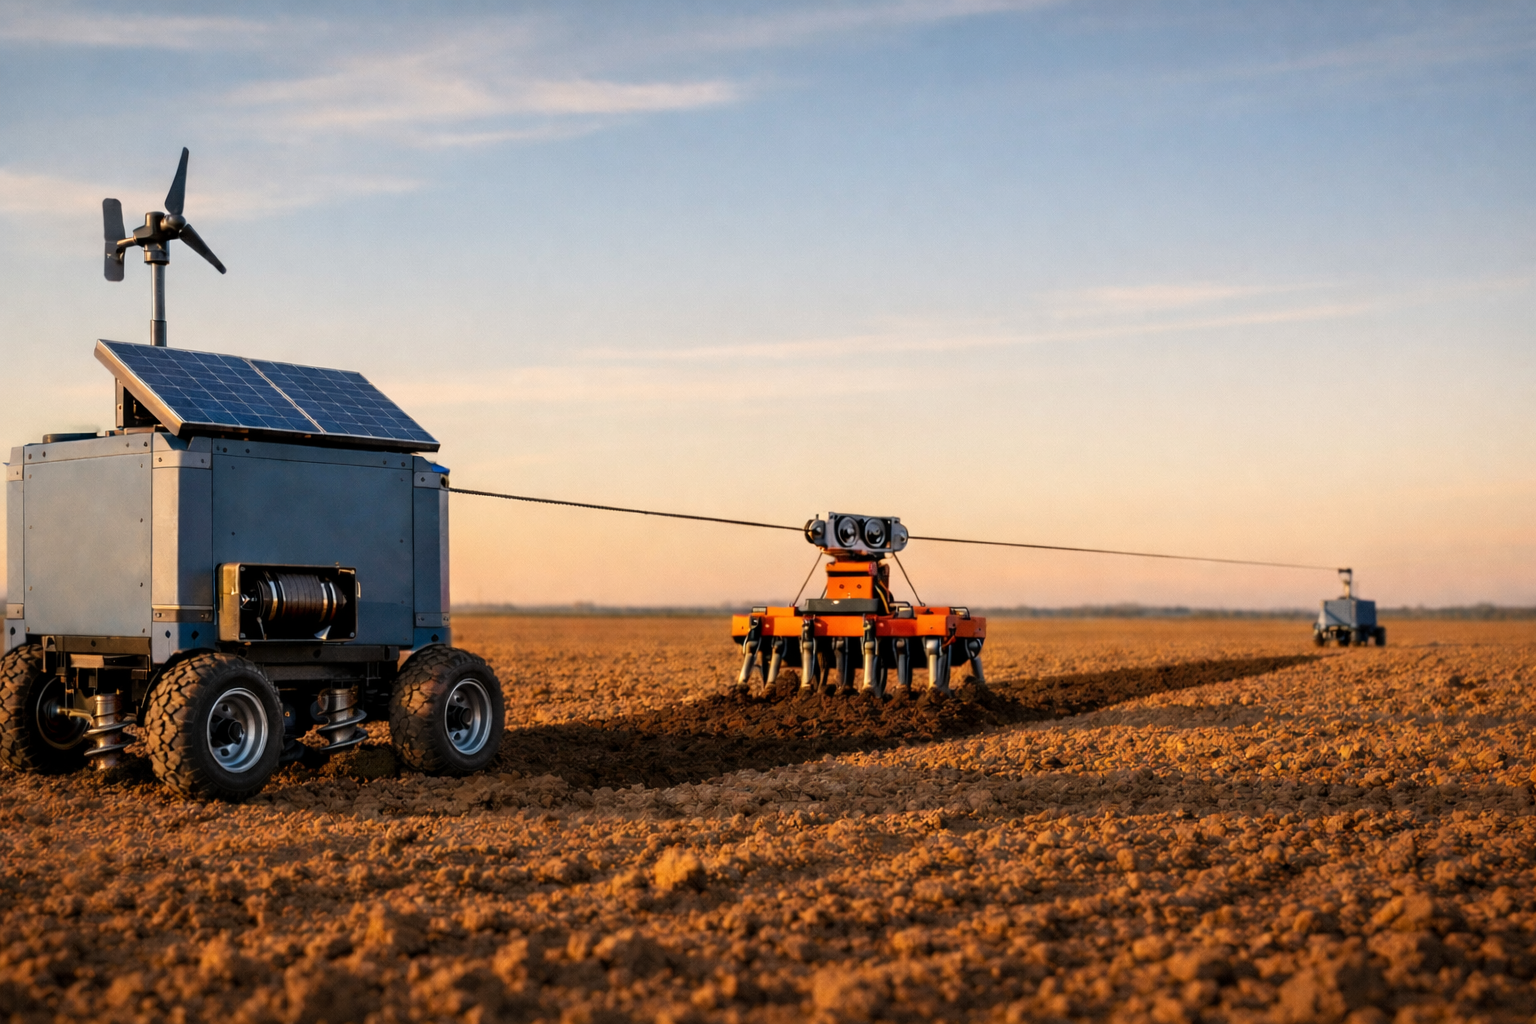
\includegraphics[width=0.92\linewidth]{F0b_hero_scene}%
}{%
  \begin{tikzpicture}
    \draw[thick,dashed,gray] (0,0) rectangle (14,5.2);
    \node[align=center,gray] at (7,2.6) {\textit{[hero rendering --- placeholder]}\\
      See \texttt{drawings/AI\_PROMPTS.md} for the image prompt.};
  \end{tikzpicture}%
}
\caption{CableTract operating in a field. The Main Unit (left) houses the winch, drivetrain, battery, PV panel and small wind turbine; the Anchor (right) is a passive helical-pile module that resists the cable reaction. A lightweight implement carriage runs along the tensioned cable across a typical \SI{50}{\meter} span. Only the carriage and the cable enter the field --- the two heavy modules stay on opposite headlands for the entire operation.}
\label{fig:f0b}
\end{figure}

\subsection{Two-module architecture}\label{sec:two-module}

\begin{figure}[H]
\centering
\resizebox{\linewidth}{!}{%
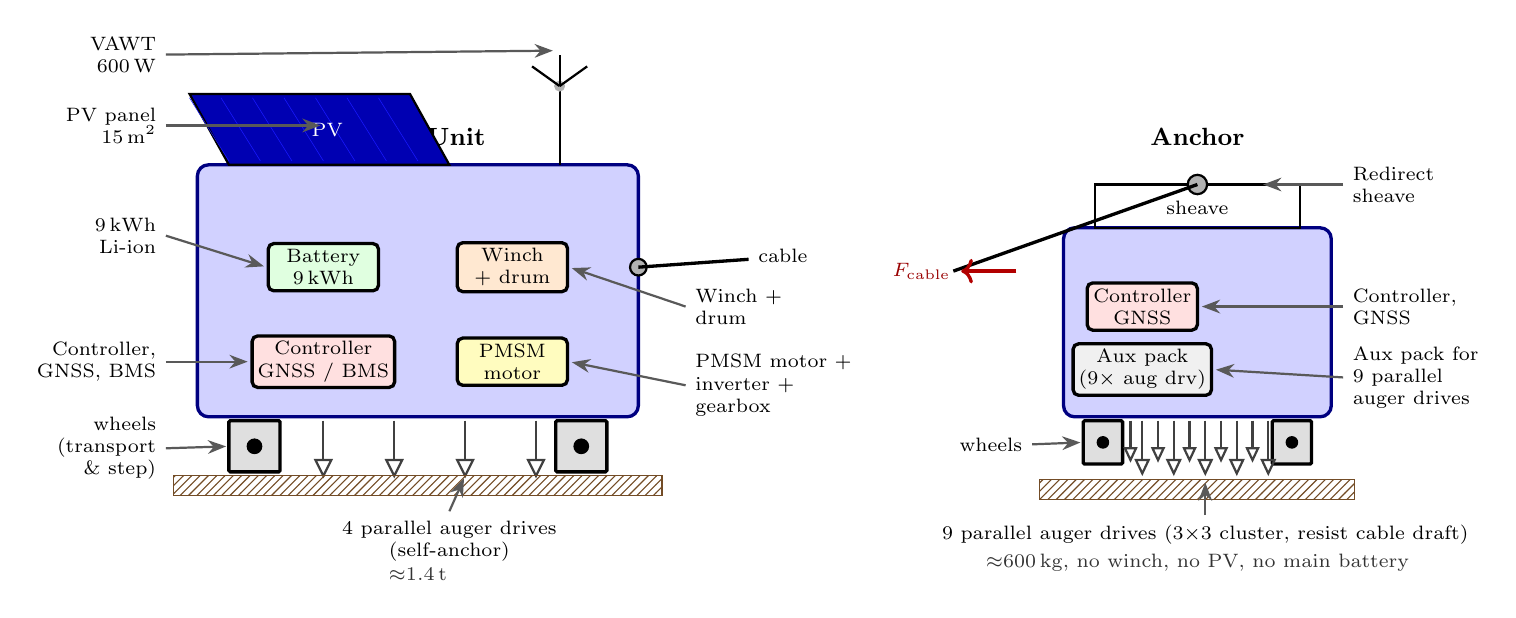
\begin{tikzpicture}[
    every node/.style={font=\footnotesize},
    subsys/.style={draw=black, very thick, rounded corners=2pt, fill=blue!8,
                   minimum width=14mm, minimum height=6mm, align=center,
                   inner sep=2pt, font=\scriptsize},
    callout/.style={->, >=Stealth, thick, gray!70!black, shorten >=1pt},
    body/.style={draw=blue!50!black, very thick, fill=blue!18, rounded corners=4pt},
    ground/.style={pattern=north east lines, pattern color=brown!60!black, draw=brown!60!black},
    wheel/.style={draw=black, very thick, fill=gray!25, rounded corners=0.5pt},
]

% =====================================================================
% LEFT PANEL: Main Unit
% =====================================================================
\begin{scope}[xshift=0cm]

% Module body (rectangle)
\draw[body] (0,0) rectangle (5.6,3.2);
\node[font=\bfseries\small] at (2.8,3.55) {Main Unit};

% PV panel on top, tilted
\draw[fill=blue!70!black, draw=black, thick]
    (0.4,3.2) -- ++(2.8,0) -- ++(-0.5,0.9) -- ++(-2.8,0) -- cycle;
\foreach \x in {0.0,0.4,0.8,1.2,1.6,2.0,2.4} {
    \draw[blue!90!white, very thin] (0.4+\x,3.25) -- (0.4+\x-0.5,4.05);
}
\node[font=\scriptsize, white] at (1.65,3.65) {PV};

% Wind turbine
\draw[thick] (4.6,3.2) -- (4.6,4.2);
\fill[gray!60] (4.6,4.2) circle (2pt);
\draw[thick] (4.6,4.2) -- ++(0.35,0.25);
\draw[thick] (4.6,4.2) -- ++(-0.35,0.25);
\draw[thick] (4.6,4.2) -- ++(0,0.4);

% Internal subsystems (boxes inside the body)
\node[subsys, fill=orange!18] (winch) at (4.0,1.9) {Winch\\+ drum};
\node[subsys, fill=yellow!25] (motor) at (4.0,0.7) {PMSM\\motor};
\node[subsys, fill=green!12] (batt)  at (1.6,1.9) {Battery\\\SI{9}{\kWh}};
\node[subsys, fill=red!12]   (ctrl)  at (1.6,0.7) {Controller\\GNSS / BMS};

% Pulley + cable exit on the right
\fill[gray!60] (5.6,1.9) circle (3pt);
\draw[thick] (5.6,1.9) circle (3pt);
\draw[very thick, black] (5.6,1.9) -- (7.0,2.0);
\node[anchor=west, font=\scriptsize] at (7.0,2.05) {cable};

% 2 wheels (transport mode + headland step) and 4 helical augers (self-anchoring)
% Wheels on the outer corners
\draw[wheel] (0.4,-0.05) rectangle (1.05,-0.7);
\fill[black] (0.725,-0.375) circle (0.1);
\draw[wheel] (4.55,-0.05) rectangle (5.2,-0.7);
\fill[black] (4.875,-0.375) circle (0.1);
% Augers between/around the wheels (deployed downward into the soil)
\foreach \x in {1.6,2.5,3.4,4.3} {
    \draw[thick, gray!50!black] (\x,-0.05) -- (\x,-0.55);
    \draw[thick, gray!50!black] (\x-0.1,-0.55) -- (\x+0.1,-0.55)
                                                -- (\x,-0.75) -- cycle;
}

% Ground line under MU
\draw[ground] (-0.3,-0.75) rectangle (5.9,-1.0);

% Callouts (external labels)
\node[anchor=east, font=\scriptsize, align=right] (lblPV) at (-0.4,3.7) {PV panel\\\SI{15}{\meter\squared}};
\draw[callout] (lblPV.east) -- (1.6,3.7);

\node[anchor=east, font=\scriptsize, align=right] (lblWind) at (-0.4,4.6) {VAWT\\\SI{600}{\watt}};
\draw[callout] (lblWind.east) -- (4.55,4.65);

\node[anchor=west, font=\scriptsize, align=left] (lblWinch) at (6.2,1.4) {Winch +\\drum};
\draw[callout] (lblWinch.west) -- (winch.east);

\node[anchor=west, font=\scriptsize, align=left] (lblMot) at (6.2,0.4) {PMSM motor +\\inverter +\\gearbox};
\draw[callout] (lblMot.west) -- (motor.east);

\node[anchor=east, font=\scriptsize, align=right] (lblBatt) at (-0.4,2.3) {\SI{9}{\kWh}\\Li-ion};
\draw[callout] (lblBatt.east) -- (batt.west);

\node[anchor=east, font=\scriptsize, align=right] (lblCtrl) at (-0.4,0.7) {Controller,\\GNSS, BMS};
\draw[callout] (lblCtrl.east) -- (ctrl.west);

\node[anchor=north, font=\scriptsize, align=center] (lblAug) at (3.2,-1.2) {4 parallel auger drives\\(self-anchor)};
\draw[callout] (lblAug.north) -- (3.4,-0.75);

\node[anchor=east, font=\scriptsize, align=right] (lblWheel) at (-0.4,-0.4) {wheels\\(transport\\\& step)};
\draw[callout] (lblWheel.east) -- (0.4,-0.375);

\node[font=\scriptsize, gray!40!black] at (2.8,-2.0) {${\approx}\SI{1.4}{\tonne}$};

\end{scope}

% =====================================================================
% RIGHT PANEL: Anchor
% =====================================================================
\begin{scope}[xshift=11cm]

% Module body
\draw[body] (0,0) rectangle (3.4,2.4);
\node[font=\bfseries\small] at (1.7,3.55) {Anchor};

% Sheave block on top
\draw[thick] (0.4,2.4) rectangle (3.0,2.95);
\fill[gray!60] (1.7,2.95) circle (3.5pt);
\draw[thick] (1.7,2.95) circle (3.5pt);
\node[font=\scriptsize] at (1.7,2.65) {sheave};

% Cable entering from left
\draw[very thick, black] (-1.4,1.85) -- (1.7,2.95);

% Internal subsystems (sparser than MU)
\node[subsys, fill=red!12] (actrl) at (1.0,1.4) {Controller\\GNSS};
\node[subsys, fill=gray!12, minimum width=12mm] (aux) at (1.0,0.6) {Aux pack\\(9$\times$ aug drv)};

% 2 wheels (headland repositioning) at the outer corners
\draw[wheel] (0.25,-0.05) rectangle (0.75,-0.6);
\fill[black] (0.5,-0.325) circle (0.08);
\draw[wheel] (2.65,-0.05) rectangle (3.15,-0.6);
\fill[black] (2.9,-0.325) circle (0.08);

% 9 helical augers in a 3-row pattern between/around the wheels
\foreach \x in {1.0,1.4,1.8,2.2,2.6} {
    \draw[thick, gray!50!black] (\x,-0.05) -- (\x,-0.55);
    \draw[thick, gray!50!black] (\x-0.08,-0.55) -- (\x+0.08,-0.55) -- (\x,-0.72) -- cycle;
}
\foreach \x in {0.85,1.2,1.6,2.0,2.4} {
    \draw[thick, gray!50!black] (\x,-0.05) -- (\x,-0.4);
    \draw[thick, gray!50!black] (\x-0.07,-0.4) -- (\x+0.07,-0.4) -- (\x,-0.55) -- cycle;
}

% Ground
\draw[ground] (-0.3,-0.8) rectangle (3.7,-1.05);

% Callouts (kept tight on the right so the resizebox doesn't crush them)
\node[anchor=west, font=\scriptsize, align=left] (lblSheave) at (3.55,2.95) {Redirect\\sheave};
\draw[callout] (lblSheave.west) -- (2.5,2.95);

\node[anchor=west, font=\scriptsize, align=left] (lblCtrlA) at (3.55,1.4) {Controller,\\GNSS};
\draw[callout] (lblCtrlA.west) -- (actrl.east);

\node[anchor=west, font=\scriptsize, align=left] (lblAux) at (3.55,0.5) {Aux pack for\\9 parallel\\auger drives};
\draw[callout] (lblAux.west) -- (aux.east);

\node[anchor=north, font=\scriptsize, align=center] (lblAugA) at (1.8,-1.25) {9 parallel auger drives (3$\times$3 cluster, resist cable draft)};
\draw[callout] (lblAugA.north) -- (1.8,-0.8);

\node[anchor=east, font=\scriptsize, align=right] (lblWhA) at (-0.4,-0.35) {wheels};
\draw[callout] (lblWhA.east) -- (0.25,-0.325);

\node[font=\scriptsize, gray!40!black] at (1.7,-1.85) {${\approx}\SI{600}{\kilogram}$, no winch, no PV, no main battery};

% Reaction force arrow
\draw[->, very thick, red!70!black] (-0.6,1.85) -- ++(-0.7,0)
    node[anchor=east, font=\scriptsize, red!60!black] {$F_{\text{cable}}$};

\end{scope}

\end{tikzpicture}%
}
\caption{The two physically separable modules of CableTract. \textbf{Left:} the \textbf{Main Unit} carries the entire active drivetrain (PMSM + winch + drum), the energy stack (\SI{9}{\kWh} battery, \SI{15}{\meter\squared} PV, \SI{600}{\watt} VAWT) and the controller, and self-anchors with four parallel auger drives during operation (one BLDC drive motor per auger, so all four insert and retract concurrently). \textbf{Right:} the \textbf{Anchor} is a passive sheave block on top of nine parallel auger drives in a 3$\times$3 cluster that together resist the full horizontal cable reaction $F_{\text{cable}}$ at the opposite headland; it carries only an auxiliary pack powering the nine drives and a controller/GNSS for headland repositioning, no winch, no PV, no main battery. The parallel-drive choice on both modules is what keeps the per-round insert/retract cycle short enough to hit the \SI{60}{\second} setup target of \cref{tab:codesigned-params}; a single-drive-head design that visited each auger sequentially would not. The asymmetric split halves the BoM and mass of the second module relative to a symmetric two-winch design.}
\label{fig:f0a}
\end{figure}

CableTract has two physically separable modules:

\begin{itemize}[leftmargin=1.6em,itemsep=0.15em]
    \item \textbf{Main Unit} (${\approx}\SI{1.4}{\tonne}$ including PV deployable): \gls{pmsm} motor + 3-phase inverter + 2-stage gearbox + \SI{8}{\milli\meter} Dyneema-on-drum winch, \SI{9}{\kWh} Li-ion pack, \SI{15}{\meter\squared} flat-plate mono-Si \gls{pv}, \SI{600}{\watt} small \gls{vawt}, controller, \gls{gnss}, \gls{bms}, and 4 parallel auger drives for self-anchoring of the Main Unit itself (one small \gls{bldc} per auger, all four cycling concurrently).
    \item \textbf{Anchor} (${\approx}\SI{600}{\kilogram}$): 9 parallel auger drives in a 3$\times$3 cluster (one \gls{bldc} per auger, with a shared auxiliary battery pack and a single controller multiplexing across the nine drivers, so all nine insert and retract concurrently in a single per-round cycle), redirect sheave block, simple electric drive for headland repositioning on its own wheels, \gls{gnss}, no main battery beyond the auxiliary auger-drive pack.
\end{itemize}

In \emph{transport mode} the Anchor docks against the \gls{mu} and the assembly behaves as a compact \SI{1.5}{\meter} wide, \SI{1}{\meter} tall electric utility vehicle that can drive between fields on farm tracks. In \emph{work mode} the Anchor walks across the field on its own electric drive and plants itself at the far headland; the \gls{mu} runs the cable across the strip; the implement carriage rolls along the cable.

\subsection{Operating cycle}\label{sec:cycle}

\begin{figure}[H]
\centering
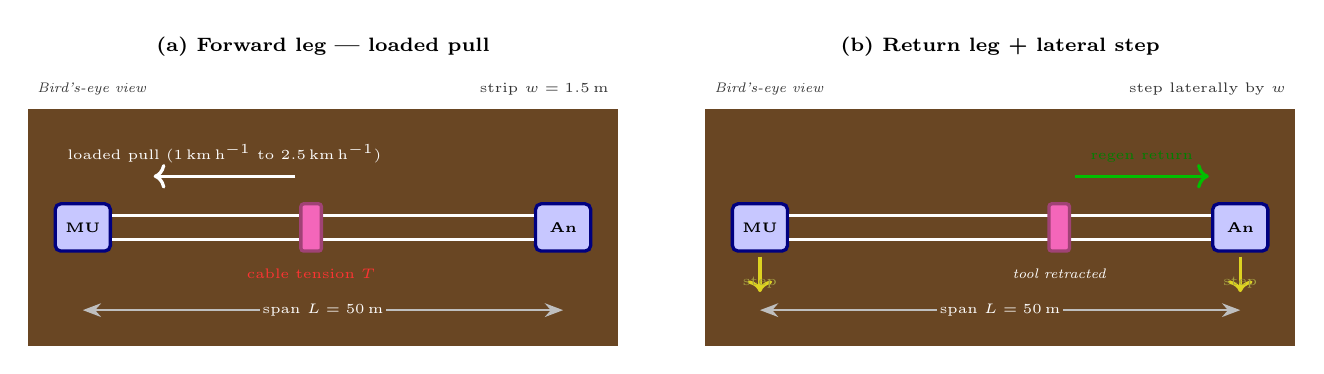
\begin{tikzpicture}[
    every node/.style={font=\scriptsize},
    mu/.style={draw=blue!50!black, very thick, fill=blue!22, rounded corners=2pt,
               minimum width=7mm, minimum height=6mm, align=center, font=\tiny\bfseries},
    anc/.style={draw=blue!50!black, very thick, fill=blue!22, rounded corners=2pt,
                minimum width=7mm, minimum height=6mm, align=center, font=\tiny\bfseries},
    impl/.style={draw=magenta!60!black, very thick, fill=magenta!60, rounded corners=1pt,
                 minimum width=2.6mm, minimum height=6mm, align=center,
                 font=\tiny\bfseries, text=white},
    field/.style={fill=brown!55!black},
    cable/.style={white, line width=1.2pt},
    dim/.style={<->, >=Stealth, gray!50!white, thick},
]

% =====================================================================
% PANEL A: Forward (loaded) leg
% =====================================================================
\begin{scope}[xshift=0cm]
% Panel title well above the field
\node[font=\scriptsize\bfseries, anchor=south] at (3.75,3.55) {(a) Forward leg --- loaded pull};

% Bird's-eye view label outside the field, above
\node[font=\tiny\itshape, gray!40!black, anchor=south west] at (0,3.05) {Bird's-eye view};
% Width tick label outside the field, above-left
\node[font=\tiny, gray!40!black, anchor=south east] at (7.5,3.05) {strip $w = \SI{1.5}{\meter}$};

% Field background
\fill[field] (0,0) rectangle (7.5,3);

% MU on left, Anchor on right
\node[mu] (mu1) at (0.7,1.5) {MU};
\node[anc] (an1) at (6.8,1.5) {An};

% Two parallel cables drawn straight horizontal across the field
\draw[cable] ($(mu1.east) + (0,0.15)$) -- ($(an1.west) + (0,0.15)$);
\draw[cable] ($(mu1.east) + (0,-0.15)$) -- ($(an1.west) + (0,-0.15)$);

% Implement carriage in the middle, riding on the cables
\node[impl] (im1) at (3.6,1.5) {};

% Motion arrow above the cables, pointing left (loaded toward MU)
\draw[->, very thick, white] (3.4,2.15) -- (1.6,2.15);
\node[white, font=\tiny, anchor=south] at (2.5,2.2) {loaded pull (\SIrange{1}{2.5}{\km\per\hour})};

% Cable tension annotation below the cables
\node[red!80!white, font=\tiny, anchor=north] at (3.6,1.1) {cable tension $T$};

% Span dimension at the very bottom of the field
\draw[dim] (mu1.south |- 0,0.45) -- (an1.south |- 0,0.45);
\node[white, font=\tiny, fill=brown!55!black, inner sep=1pt]
    at (3.75,0.45) {span $L = \SI{50}{\meter}$};
\end{scope}

% =====================================================================
% PANEL B: Return (unloaded) leg + lateral step
% =====================================================================
\begin{scope}[xshift=8.6cm]
\node[font=\scriptsize\bfseries, anchor=south] at (3.75,3.55) {(b) Return leg + lateral step};

\node[font=\tiny\itshape, gray!40!black, anchor=south west] at (0,3.05) {Bird's-eye view};
\node[font=\tiny, gray!40!black, anchor=south east] at (7.5,3.05) {step laterally by $w$};

\fill[field] (0,0) rectangle (7.5,3);

\node[mu] (mu2) at (0.7,1.5) {MU};
\node[anc] (an2) at (6.8,1.5) {An};

\draw[cable] ($(mu2.east) + (0,0.15)$) -- ($(an2.west) + (0,0.15)$);
\draw[cable] ($(mu2.east) + (0,-0.15)$) -- ($(an2.west) + (0,-0.15)$);

% Implement returning toward anchor (closer to right side)
\node[impl] (im2) at (4.5,1.5) {};

% Motion arrow above the cables, pointing right (unloaded back to anchor)
\draw[->, very thick, green!75!black] (4.7,2.15) -- (6.4,2.15);
\node[green!50!black, font=\tiny, anchor=south] at (5.55,2.2) {regen return};

% Tool retracted label, below the implement
\node[white, font=\tiny\itshape, anchor=north] at (4.5,1.1) {tool retracted};

% Lateral step arrows on both modules — pointing down (into the page, perpendicular to cable)
\draw[->, very thick, yellow!85!black] (mu2.south) ++(0,-0.05) -- ++(0,-0.45);
\node[yellow!60!black, font=\tiny, anchor=north] at (0.7,1.0) {step};
\draw[->, very thick, yellow!85!black] (an2.south) ++(0,-0.05) -- ++(0,-0.45);
\node[yellow!60!black, font=\tiny, anchor=north] at (6.8,1.0) {step};

% Span dimension at the very bottom of the field
\draw[dim] (mu2.south |- 0,0.45) -- (an2.south |- 0,0.45);
\node[white, font=\tiny, fill=brown!55!black, inner sep=1pt]
    at (3.75,0.45) {span $L = \SI{50}{\meter}$};
\end{scope}

\end{tikzpicture}
\caption{One round of the CableTract operating cycle, bird's-eye view. \textbf{(a) Forward leg:} the Main Unit's winch reels in cable, the implement carriage moves loaded toward the MU at \SIrange{1}{2.5}{\kilo\meter\per\hour}, the working tool engages the soil, and the full draft $F_{\text{draft}}$ is reacted at the Anchor as $F_{\text{reaction}}$. \textbf{(b) Return leg:} the tool retracts, the cable goes slack, and the carriage rolls back to the Anchor end (downhill assist or active pull-back). The unloaded return leg can recover kinetic / potential energy via four-quadrant motor operation (\cref{sec:regen}, \cref{sec:variant-regen}). After the return, the MU and the Anchor each step laterally by one strip width (\SI{1.5}{\meter}) along the headland and the cycle repeats on the next strip.}
\label{fig:f0c}
\end{figure}

One round of work proceeds as:

\begin{enumerate}[leftmargin=1.6em,itemsep=0.1em]
    \item The implement carriage starts at the Anchor end with the working tool engaged.
    \item The \gls{mu}'s winch reels in cable. The carriage moves loaded toward the \gls{mu} at the operating speed (typically \SIrange{1}{2.5}{\kilo\meter\per\hour}).
    \item At the \gls{mu} end, the carriage tool retracts, the cable goes slack, and the carriage either gravity-rolls back (downhill) or is towed back by a thin return line. The unloaded return leg can recover kinetic / potential energy via four-quadrant motor operation (regenerative braking, \cref{sec:regen}).
    \item The \gls{mu} and Anchor each step laterally by one strip width along the headland.
    \item Setup repeats on the next strip.
\end{enumerate}

Typical numbers for the codesigned reference: span \SI{50}{\meter}, strip width \SI{1.5}{\meter}, carriage mass ${\approx}\SI{250}{\kilogram}$, operating speed \SI{1.5}{\kilo\meter\per\hour}, setup time per round \SI{60}{\second}.

\subsection{Why an asymmetric architecture}\label{sec:asymmetry}

\begin{figure}[H]
\centering
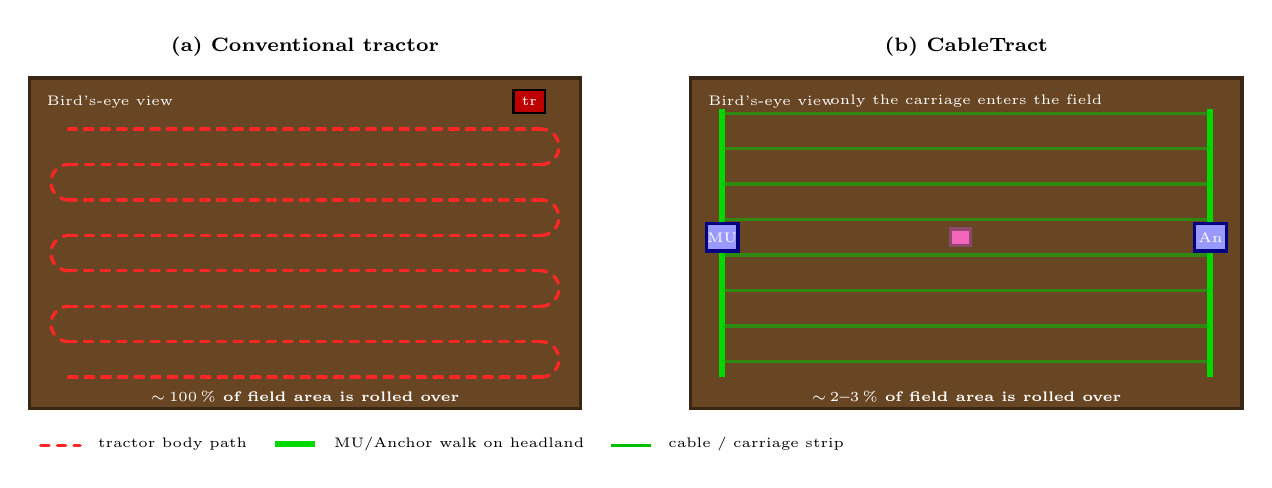
\begin{tikzpicture}[
    every node/.style={font=\tiny},
    field/.style={fill=brown!55!black, draw=brown!30!black, very thick},
    tractor/.style={red!85!white, very thick, dashed, line cap=round},
    cable/.style={green!75!black, very thick},
    ctcarriage/.style={green!85!black, line width=2.2pt},
    legend/.style={font=\tiny, anchor=west},
]

% =====================================================================
% PANEL A: Conventional tractor — snake path covering the whole field
% =====================================================================
\begin{scope}[xshift=0cm]
\node[font=\scriptsize\bfseries, anchor=south] at (3.5,4.35) {(a) Conventional tractor};
\fill[field] (0,0) rectangle (7,4.2);
\node[white, font=\tiny, anchor=north west] at (0.1,4.1) {Bird's-eye view};

% Snake / boustrophedon path covering the whole field
% 8 horizontal sweeps connected by U-turns
\foreach \i [evaluate=\i as \y using {0.4+0.45*\i}] in {0,1,...,7} {
    \ifodd\i
        \draw[tractor] (6.5,\y) -- (0.5,\y);
    \else
        \draw[tractor] (0.5,\y) -- (6.5,\y);
    \fi
}
% U-turns at the ends
\foreach \i in {0,2,4,6} {
    \pgfmathsetmacro{\ya}{0.4+0.45*\i}
    \draw[tractor] (6.5,\ya) arc (-90:90:0.225);
}
\foreach \i in {1,3,5} {
    \pgfmathsetmacro{\ya}{0.4+0.45*\i}
    \draw[tractor] (0.5,\ya) arc (270:90:0.225);
}

% Tractor icon at top-right indicating direction
\draw[fill=red!75!black, draw=black, thick]
    (6.15,3.75) rectangle (6.55,4.05);
\node[font=\tiny, white] at (6.35,3.9) {tr};

% Compacted area annotation
\node[white, font=\tiny\bfseries, align=center] at (3.5,0.15)
    {${\sim}\,100\,\%$ of field area is rolled over};
\end{scope}

% =====================================================================
% PANEL B: CableTract — straight headland edge path only
% =====================================================================
\begin{scope}[xshift=8.4cm]
\node[font=\scriptsize\bfseries, anchor=south] at (3.5,4.35) {(b) CableTract};
\fill[field] (0,0) rectangle (7,4.2);
\node[white, font=\tiny, anchor=north west] at (0.1,4.1) {Bird's-eye view};

% MU and Anchor walking along left and right headlands respectively
\draw[ctcarriage] (0.4,0.4) -- (0.4,3.8);
\draw[ctcarriage] (6.6,0.4) -- (6.6,3.8);

% Cable / strip indications across the field at sample positions
\foreach \y in {0.6,1.05,1.5,1.95,2.4,2.85,3.3,3.75} {
    \draw[cable, opacity=0.55] (0.4,\y) -- (6.6,\y);
}

% MU and Anchor module icons (current strip)
\draw[fill=blue!40, draw=blue!50!black, very thick] (0.2,2.0) rectangle (0.6,2.35);
\node[white, font=\tiny] at (0.4,2.175) {MU};
\draw[fill=blue!40, draw=blue!50!black, very thick] (6.4,2.0) rectangle (6.8,2.35);
\node[white, font=\tiny] at (6.6,2.175) {An};

% Implement carriage on the active cable
\draw[fill=magenta!60!white, draw=magenta!50!black, very thick]
    (3.3,2.07) rectangle (3.55,2.28);

% Annotation: only carriage rolls
\node[white, font=\tiny\bfseries, align=center] at (3.5,0.15)
    {${\sim}\,2\text{--}3\,\%$ of field area is rolled over};
\node[white, font=\tiny, align=center] at (3.5,3.9)
    {only the carriage enters the field};
\end{scope}

% =====================================================================
% Caption-style legend below both panels
% =====================================================================
\node[legend, anchor=west] at (0,-0.45) {%
    \tikz{\draw[tractor] (0,0)--(0.5,0);} \, tractor body path
    \quad
    \tikz{\draw[ctcarriage] (0,0)--(0.5,0);} \, MU/Anchor walk on headland
    \quad
    \tikz{\draw[cable] (0,0)--(0.5,0);} \, cable / carriage strip};

\end{tikzpicture}
\caption{Why an asymmetric, headland-only architecture wins on compaction. \textbf{(a)} A conventional tractor must drive a boustrophedon (snake) path that covers essentially the entire field area at least once per pass --- every square metre of the soil is rolled over by a \SIrange{1}{4}{\tonne} body. \textbf{(b)} CableTract keeps the Main Unit and the Anchor on opposite headlands and runs only a \SI{250}{\kilogram} carriage along the cable across the field; over a full season the rolled-over fraction collapses to ${\sim}2\text{--}3\,\%$ of the field area (essentially the carriage strips). The contact-pressure $\times$ pass-count integrand drops by a much larger factor still --- see \cref{fig:f12} and \cref{sec:r-c1} for the quantitative compaction model.}
\label{fig:f0d}
\end{figure}

Symmetric cable-traction systems (like the Orlando--Zoffoli patent~\cite{orlando2014patent}) need two winches, two batteries, two motor controllers, and two sets of high-power electronics. The asymmetric CableTract design moves all the power electronics into one module and lets the second module be a simple anchored drive. This roughly halves the \gls{bom} of the second module, halves its mass, and removes one of the two failure-prone winches.

The price of the asymmetry is that the cable reaction is one-sided. The Anchor must hold the entire horizontal draft against the soil. We address this with helical screw piles (\cref{sec:anchor}) and quantify the per-auger requirement against the conservative end of the helical-pile lateral capacity literature, so that every auger count we report is a worst-case envelope.

\subsection{Co-designed implement library}\label{sec:codesign}

The single most impactful design choice in this paper is \textbf{building implements for CableTract instead of borrowing them from a tractor}. A conventional 8-row planter is built to survive the hitch loads of a \SI{4}{\tonne} tractor at \SI{9}{\kilo\meter\per\hour} on a \SI{1.5}{\meter} depth-control wheel; it weighs \SI{800}{\kilogram} and pulls \SI{3.9}{\kilo\newton} of draft. CableTract neither needs nor can usefully exploit any of those numbers. The codesigned 4-row planter\footnote{Tabulated in \texttt{data/asabe\_d497\_cabletract.csv} of the repository.} is sized for a \SI{1.5}{\meter} strip, \SI{2}{\kilo\meter\per\hour} operating speed, $0.85\times$ the conventional working depth, and a carriage frame freed from tractor hitch loads. Its \gls{p50} draft drops from \SI{3.88}{\kilo\newton} to \SI{1.94}{\kilo\newton} --- a \textbf{factor of 2.0 reduction}, achieved purely by re-sizing.

The 10-implement codesigned library and the achieved draft reduction (\cref{tab:codesigned-library}):

\begin{table}[H]
\centering\small
\caption{Codesigned implement library, \gls{p50} draft reduction relative to the conventional \gls{asabe} D497.7~\cite{asabe-d497} entry it derives from. Medium-texture soil, samples from \cref{sec:soil-monte-carlo}.}\label{tab:codesigned-library}
\resizebox{\textwidth}{!}{%
\begin{tabular}{lllrlrr}
\toprule
Operation & Conventional implement & & Conv. P50 (N) & Codesigned implement & Codes. P50 (N) & Reduction \\
\midrule
primary tillage   & subsoiler 1-shank      &  & 10\,981 & narrow ripper 1-shank (\SI{15}{\centi\meter}) & 3\,022 & $0.28\times$ \\
primary tillage   & chisel plow 7-tool     &  & 14\,174 & narrow chisel 4-tool (\SI{12}{\centi\meter}) & 4\,219 & $0.30\times$ \\
secondary tillage & disk harrow \SI{2.5}{\meter} tandem & & 8\,428  & narrow disk \SI{1.5}{\meter} & 3\,231 & $0.38\times$ \\
secondary tillage & field cultivator 11 S-tine & & 3\,175 & narrow cultivator 6-tool & 1\,347 & $0.42\times$ \\
primary tillage   & sweep plow \SI{3}{\meter} & & 15\,412 & narrow sweep \SI{1.5}{\meter} & 5\,174 & $0.34\times$ \\
seeding           & row planter 8-row      &  & 3\,876  & codesigned planter 4-row & 1\,935 & $0.50\times$ \\
seeding           & grain drill 24-row     &  & 9\,302  & codesigned drill 12-row & 4\,650 & $0.50\times$ \\
weeding           & rotary hoe \SI{4}{\meter} &  & 2\,251 & codesigned rotary hoe \SI{2}{\meter} & 788 & $0.35\times$ \\
spraying          & boom sprayer           &  & 204     & codesigned sprayer \SI{1}{\meter}   & 143 & $0.70\times$ \\
mowing            & rotary mower \SI{3}{\meter} & & 1\,452 & codesigned mower \SI{1.5}{\meter} & 523 & $0.36\times$ \\
\midrule
\multicolumn{6}{r}{\textbf{Median reduction}} & $\boldsymbol{0.37\times}$ \\
\bottomrule
\end{tabular}%
}
\end{table}

\textbf{Median reduction across the 10 operations: $0.37\times$ (${\approx}\,63\%$ lower draft).} The reduction comes from three independent levers, each defensible from the \gls{asabe} D497.7 equation
\begin{equation}\label{eq:d497}
D \;=\; F_{\!i} \,(A + B v + C v^{2})\, W \, T,
\end{equation}
where $D$ is draft (N), $v$ is field speed (\si{\kilo\meter\per\hour}), $W$ is the implement's natural width unit, $T$ is working depth, $F_{\!i}$ is a soil-texture multiplier, and $(A,B,C)$ are machine-specific coefficients. The three levers are:

\begin{enumerate}[leftmargin=1.6em,itemsep=0.15em]
    \item \textbf{Width.} Halving $W$ halves draft directly. The cable architecture wants narrow strips because the \SI{50}{\meter} cable span and the \SI{1.5}{\meter} strip width together produce a \SI{75}{\meter\squared} working envelope per round, which matches the carriage's mechanical envelope.
    \item \textbf{Speed.} The $B v + C v^{2}$ terms grow rapidly with speed. Operating at \SIrange{1.5}{2.5}{\kilo\meter\per\hour} instead of \SIrange{5}{9}{\kilo\meter\per\hour} drops the speed-dependent draft contribution by roughly 60\,\%. This is a \emph{physical} gain, not a marketing claim, and it is the same lever any slow-moving robot exploits. \Cref{fig:f5} quantifies the saving.
    \item \textbf{Depth.} Working at $0.85\times$ the conventional depth drops $T$ by 15\,\% directly. CableTract takes one extra pass per season for primary tillage to compensate, which is bookkept in the energy and economics models.
\end{enumerate}

The price of the codesigned library is that the farmer cannot take a CableTract to a neighbour's field and hook up the neighbour's plough. CableTract is sold as a \emph{system} --- Main Unit + Anchor + carriage + implements --- not as a generic cable robot that accepts off-the-shelf tools. This is the same business model as Farmdroid, EcoRobotix, and Naio.

% ====================================================================
\section{Research Questions}\label{sec:rqs}
% ====================================================================

We organise the analysis around four claims and seven research questions. The four claims are the headline assertions the paper defends with code-traceable numbers; the seven research questions decompose each claim into the operational regime, the physical mechanism, and the binding constraint.

\paragraph{C1 --- Compaction.} CableTract reduces in-field compacted area by at least 90\,\% and the contact-energy index by at least $20\times$ compared with an \SI{80}{hp} \gls{wd} diesel tractor on the same field, because only the lightweight carriage rolls inside the field while the \gls{mu} and Anchor stay on the headland.

\paragraph{C2 --- Energy.} With a co-designed implement library, CableTract operates at ${\approx}\SI{0.9}{\kWh\per\decare}$ (${\approx}\SI{9}{\kWh\per\hectare}$), roughly an order of magnitude below a diesel tractor at the same operation, driven primarily by (i) the absence of dead-weight transport, (ii) the $v^2$ speed reduction, and (iii) the narrow-strip width.

\paragraph{C3 --- Off-grid.} Off-grid operation is achievable in solar-rich climates (Konya, Ludhiana, São Paulo) with \SI{15}{\meter\squared} of \gls{pv} and a \SI{9}{\kWh} battery, conditional in Mediterranean ones (Palencia, Des Moines), and not achievable at any practical hardware scale in northern temperate climates (Beauce) under a \SI{6}{\hour\per day} duty cycle. The off-grid claim is \emph{climate-conditional}, not categorical.

\paragraph{C4 --- Economics and life-cycle CO\textsubscript{2}.} The codesigned CableTract is \gls{npv}-positive across the full \SIrange{1}{100}{\hectare} farm-size range at all three discount rates we test (5/8/12\,\%), with discounted payback under one year at $\geq\!\SI{25}{\hectare}$ annual operating area, and lifecycle CO\textsubscript{2} of \SI{14.6}{\kilogram\per\hectare\per\year} versus 32.5 for diesel --- a $2.2\times$ improvement that does not depend on grid decarbonisation.

\medskip
The research questions:

\begin{description}[leftmargin=2.0em,style=nextline,itemsep=0.25em]
    \item[\gls{rq}1] What is the compacted-area reduction and contact-energy reduction across rectangle, L-shape, and irregular-concave field classes?
    \item[\gls{rq}2] What energy per decare does the codesigned reference achieve, and how does it decompose between mechanical work, drivetrain losses, and dead-weight motion?
    \item[\gls{rq}3] Under which combinations of annual \gls{ghi}, panel area, and battery capacity is the system off-grid capable?
    \item[\gls{rq}4] For which operation classes is the architecture most favourable, and where does the helical-pile anchor envelope bind?
    \item[\gls{rq}5] How do polygon shape and size erode the throughput on real fields?
    \item[\gls{rq}6] Is the codesigned reference Pareto-optimal on (CAPEX $\times$ throughput $\times$ payback $\times$ energy intensity), or does it leave headroom?
    \item[\gls{rq}7] Across the (annual \gls{ghi} $\times$ farm size) plane, where is CableTract \gls{npv}-positive against diesel, and where does the off-grid feasibility envelope bind first?
\end{description}

% ====================================================================
\section{Methods}\label{sec:methods}
% ====================================================================

\subsection{Modelling philosophy}\label{sec:philosophy}

The analysis is parametric and designed to expose its assumptions. Every parameter has units, every default value has a citation in a bundled data file, and every claim in \cref{sec:results} has a per-figure CSV companion with the underlying numbers.\footnote{Full source and data: \cabletractrepo} We do not attempt high-fidelity soil-tool dynamics, full closed-loop control simulation, or finite-element cable modelling. We use first-principles work-energy balances, the standard \gls{asabe} D497.7 implement-draft equation, an hourly \gls{tmy}-based PV+battery simulator, a static contact-pressure compaction model, a discounted-cash-flow economics engine, and global Sobol sensitivity over 20 inputs. This is the appropriate fidelity for an early-stage feasibility study.

Every higher-level analysis is composed on top of one atomic computation that takes a parameter set and returns a result record. The energy simulator (\cref{sec:energy}), the global sensitivity decomposition (\cref{sec:sobol}), the architectural variants (\cref{sec:ml}), and the operating envelope (\cref{sec:envelope}) are all callers of this same routine. Every figure is therefore re-derived from a single physics-and-economics chain rather than from parallel approximations that drift apart.

\subsection{Codesigned reference parameter set}\label{sec:codesigned-ref}

The codesigned reference is the single system the rest of the paper analyses. It is \emph{the} baseline: there is no other parameter set we report headline numbers on, so every result in \cref{sec:results} can be traced back to the values in \cref{tab:codesigned-params}, which lists each entry together with a one-line engineering justification.

\begin{table}[H]
\centering\small
\caption{Codesigned reference parameter set. Used unchanged in every figure, table, and headline number in the paper.}\label{tab:codesigned-params}
\begin{tabularx}{\textwidth}{lrX}
\toprule
Parameter & Value & Notes \\
\midrule
span (\si{\meter}) & 50 & Anchor-to-Main-Unit cable distance \\
strip width (\si{\meter}) & 1.5 & Matches the codesigned implement library \\
carriage mass (N equiv.) & 600 & Lightweight steel cylinder + tool mount \\
draft load \gls{p50} (N) & 1\,800 & Median across the 10 codesigned implements \\
system travel mass (N equiv.) & 2\,200 & MU + Anchor + battery + PV \\
drivetrain efficiency (lumped) & 0.50 & Decomposed into 6 components in \cref{sec:drivetrain} \\
\gls{pv} area (\si{\meter\squared}) & 15 & Mono-Si flat plate, deployable \\
wind generator (W) & 100 & Helix \gls{vawt}, $C_p = 0.30$ \\
setup time per round (\si{\second}) & 60 & Anchor placement + cable spool + carriage hookup \\
battery (\si{\kWh}) & 9 & Li-ion, 96/96\,\% charge/discharge eff. \\
operating window (\si{\hour\per day}) & 10 & Daily total work window \\
operating days/yr & 170 & Standard EU agronomic calendar \\
diesel reference fuel (\si{\litre\per\decare}) & 1.2 & Mid-range field operation (\SI{12}{\litre\per\hectare})~\cite{siemens1999machinery,asabe-d497} \\
diesel price (\si{\EUR\per\litre}) & 1.40 & EU 2024 agricultural diesel \\
capex CableTract (\si{\EUR}) & 35\,570 & Itemised in \cref{sec:economics} \\
project horizon (\si{\year}) & 15 & Matches Kubota / Monarch warranty bands \\
discount rate (\%) & 8 & EU farm equipment loan rate \\
\bottomrule
\end{tabularx}
\end{table}

\subsection{Pass model}\label{sec:pass-model}

For one round of work, useful mechanical work is
\begin{equation}\label{eq:pass}
E_{\text{mech,round}} \;=\; F_d\,L \;+\; F_i\,L \;+\; F_s\,W,
\end{equation}
where $F_d$ is the implement draft (N), $F_i$ the carriage-plus-cable transport load (N), $F_s$ the system-weight equivalent travel load (N), $L$ the cable span (m), and $W$ the lateral repositioning distance per round (m). For the codesigned reference, $F_d L \approx 90\%$ of the round work, so the dead-weight saving relative to a tractor (where $F_s$ dwarfs $F_d$) is the dominant energy lever.

\subsection{Cable mechanics, drivetrain, anchor}\label{sec:physics}

The cable mechanics and drivetrain model are verified against 22 analytic invariants (sag monotonicity, Hooke's law in the elastic regime, energy conservation on the regen leg, and others).\footnote{Test suite: \texttt{tests/test\_physics.py} in the repository.}

\subsubsection{Decomposed drivetrain efficiency}\label{sec:drivetrain}

A lumped winch efficiency $\eta_w \approx 0.5$ is the most common single-parameter shortcut in agricultural-electrification work. It collapses six independent loss mechanisms --- motor copper losses, inverter switching losses, gearbox friction, drum tension losses, pulley redirect losses, cable elongation hysteresis --- into one number, which a global sensitivity analysis (\cref{sec:sobol}) would then assign almost all of the variance to. The chain we use in this paper is the explicit product of those six components, each independently sourced from a datasheet or a published engineering standard:

\begin{equation}\label{eq:eta-chain}
\eta_{\text{drivetrain}} \;=\; \eta_{\text{motor}} \,\eta_{\text{ctrl}}\, \eta_{\text{gearbox}} \,\eta_{\text{drum}}\, \eta_{\text{pulley}}\, \eta_{\text{cable}}.
\end{equation}

Two presets are bundled (\cref{tab:eta-decomposition}); the ``baseline'' product matches the lumped 0.5 by construction, and ``premium'' recovers ${\approx}71\%$. The global sensitivity analysis in \cref{sec:sobol} then samples each component independently, so the Sobol decomposition sees six separate variance contributors instead of one undefended fudge factor.

\begin{table}[H]
\centering\small
\caption{Decomposed drivetrain efficiency. Baseline product reproduces the lumped 0.5; premium recovers 0.71.}\label{tab:eta-decomposition}
\begin{tabularx}{\textwidth}{Xrrl}
\toprule
Component & Baseline (low-cost) & Premium (best-of-class) & Source \\
\midrule
\gls{pmsm} motor              & 0.85 & 0.93 & \cite{asabe-ep496} \\
Three-phase inverter           & 0.92 & 0.96 & \cite{asabe-ep496} \\
2-stage planetary gearbox      & 0.88 & 0.95 & drive-vendor data \\
Drum capstan + bending         & 0.88 & 0.95 & \cite{feyrer2015wireropes} \\
Redirect sheave block          & 0.90 & 0.95 & \cite{feyrer2015wireropes} \\
Cable cyclic loss              & 0.92 & 0.97 & Marlow Excel D12 datasheet \\
\midrule
\textbf{Product}               & \textbf{0.50} & \textbf{0.71} & --- \\
\bottomrule
\end{tabularx}
\end{table}

\subsubsection{Catenary sag}\label{sec:catenary}

The first geometric requirement for any cable-based field robot is that the cable must not sag into the soil. If midspan sag exceeds the implement-attachment height, the geometry breaks before any draft, energy, or economics question can be asked. \Cref{fig:f1} resolves this with a closed-form bound: it computes the minimum horizontal tension required to keep midspan sag below the depth-control clearance budget, as a function of cable material, span, and self-weight.

A perfectly flexible cable of self-weight $w$ (\si{\newton\per\meter}) hung between two supports a horizontal distance $L$ apart at horizontal tension $T_h$ takes the catenary shape~\cite{irvine1981cables}
\begin{equation}\label{eq:catenary}
y(x) \;=\; a\bigl(\cosh(x/a)-1\bigr), \qquad a \;=\; T_h / w,
\end{equation}
with midspan sag
\begin{equation}\label{eq:sag-exact}
s \;=\; a\!\left(\cosh\!\left(\frac{L}{2a}\right) - 1\right).
\end{equation}
For $w L / (2 T_h) < 0.3$ the parabolic limit
\begin{equation}\label{eq:sag-parabolic}
s \;\approx\; \frac{w L^{2}}{8 T_h}
\end{equation}
is accurate to 1\,\%. Both forms are computed and cross-checked at every operating point.

\Cref{fig:f1} sweeps horizontal cable tension from \SI{0.5}{\kilo\newton} to \SI{25}{\kilo\newton} for steel 6$\times$19 \gls{iwrc}, Dyneema SK78 12-strand, and Spectra 1000 fibre rope (all \SI{8}{\milli\meter} nominal) at three spans $L \in \{50, 75, 100\}\,\si{\meter}$.\footnote{Mechanical properties from manufacturer datasheets, tabulated in \texttt{data/cable\_props.csv}.}

\begin{figure}[H]
\centering

\includegraphics[width=0.85\linewidth]{F1_cable_sag}
\caption{Catenary sag versus horizontal cable tension for three rope materials at three spans. Synthetic-fibre rope (Dyneema or Spectra) at $\geq\SI{5}{\kilo\newton}$ pretension keeps midspan sag within the $\pm\SI{2}{\centi\meter}$ depth-control envelope for any span up to \SI{100}{\meter}; steel cable of equivalent breaking strength requires ${\approx}\SI{25}{\kilo\newton}$ to meet the same tolerance because of its $5\times$ higher self-weight per unit length.}
\label{fig:f1}
\end{figure}

\textbf{What this gives the rest of the paper.} \Cref{fig:f1} narrows the design choice to synthetic rope and quantifies the minimum working tension as a function of span. CableTract uses \SI{8}{\milli\meter} Dyneema throughout. The minimum-tension number flows into \cref{sec:tension-balance} (which side of the draft-bound vs sag-bound regime are we in?) and into \cref{sec:anchor} (the helical-pile capacity must absorb the horizontal tension we just selected).

\subsubsection{Tension balance and operating regime}\label{sec:tension-balance}

The implement carriage's own depth-control mechanism --- not the cable --- sets tilling depth. The cable transmits the horizontal draft $F_d$ and stays clear of the soil. Two regimes arise:

\begin{itemize}[leftmargin=1.6em,itemsep=0.15em]
    \item \textbf{Draft-bound:} $F_d$ is large enough that the resulting horizontal tension keeps midspan sag below the clearance budget $h_p - c_{\min}$. Horizontal tension equals $F_d$, anchor sees ${\approx}F_d$.
    \item \textbf{Sag-bound:} $F_d$ is too small to keep the cable taut against its own weight. The Main Unit over-tensions to $T_{\text{sag,min}}$. The anchor sees this larger tension.
\end{itemize}

The tension-balance solver detects which regime applies at each operating point and reports the tensions seen by both ends of the cable. \Cref{fig:f2} sweeps draft from \SI{200}{\newton} to \SI{4000}{\newton} at \SI{8}{\milli\meter} Dyneema, span \SI{50}{\meter}, $h_p = \SI{1.5}{\meter}$, with the per-auger Anchor capacity bands overlaid.

\subsubsection{Anchor reaction envelope}\label{sec:anchor}

The asymmetric architecture of \cref{sec:asymmetry} only works if the lighter Anchor module can geotechnically resist the cable reaction. A mass-anchored solution would force the Anchor to weigh as much as a small tractor, which would defeat the architecture's selling point. We therefore replace mass anchoring with helical screw piles and quantify how many augers are required at each draft level. This is the load-bearing question behind the ``CableTract is mechanically possible'' claim.

The literature on lateral capacity of helical piles spans nearly two orders of magnitude depending on soil density, shaft fixity, and the chosen serviceability limit. At the conservative end, the 4-pile group raft tests of \textbf{Khand et al.\ (2024)}~\cite{khand2024helical} imply per-pile lateral capacities on the order of \SI{400}{\newton} for short helical piles in \emph{loose} sand at strict deflection thresholds with free-head boundary conditions. At the realistic end, the \textbf{Magnum Piering 2024 design tables}~\cite{magnum2024fixed} report allowable lateral capacities of \SIrange{14}{20}{\kilo\newton} per small fixed-head helical pile in medium-dense sand (SPT $N \approx 10$--$30$) at the IBC2021 \SI{1}{inch} deflection limit, and the industry-standard CHANCE Technical Design Manual~\cite{chance2024manual} brackets the same range. We deliberately adopt the conservative end of this literature --- \SI{400}{\newton} per auger at a working safety factor of 1.15 --- as our nominal per-auger capacity, so that every auger count quoted below is a worst-case envelope. The codesigned 9-auger Anchor therefore carries a $5\times$--$10\times$ implicit margin under the medium-dense fixed-head conditions a real installer would target.

\begin{figure}[H]
\centering

\includegraphics[width=0.85\linewidth]{F2_anchor_envelope}
\caption{Anchor reaction envelope plotted against \emph{two} per-auger lateral capacity references that span the published range. \textbf{Dashed red bands (Khand et al.\ 2024~\cite{khand2024helical})}: \SI{400}{\newton} per 30~cm helical pile in \emph{loose} sand, free-head, strict deflection limit (the per-pile interpretation of the 4-pile raft tests in that paper) --- the worst-case bound. \textbf{Solid blue bands (Magnum Piering 2024~\cite{magnum2024fixed}, with~\cite{chance2024manual} as a corroborating manual reference)}: \SI{2}{\kilo\newton} per pile, taken as a conservative downscale of the \SIrange{14}{20}{\kilo\newton} fixed-head capacity reported for medium-dense sand at the IBC2021 \SI{1}{inch} deflection limit --- the realistic engineering reference. The working safety factor is 1.15 in both envelope families. The codesigned reference (P50 \SI{1.8}{\kilo\newton}, P90 \SI{3.0}{\kilo\newton}) requires 6 and 9 augers on the worst-case Khand envelope --- the design uses 9 augers and is therefore \emph{just} sized for its heaviest operation in loose sand --- and only 2 augers on the realistic Magnum envelope, leaving a $4.5\times$ implicit margin. A conventional implement library at \SIrange{8}{14}{\kilo\newton} (disk harrow to moldboard plow) would require 24--41 augers on the loose-sand bound and 5--9 augers on the medium-dense bound. CableTract's design choice is therefore \emph{robust}: in worst-case soil the codesigned library is what keeps the Anchor envelope feasible, and in typical soil it converts the same Anchor into a comfortable margin instead of a binding constraint.}
\label{fig:f2}
\end{figure}

\textbf{Findings.} Working from the per-implement P50/P90 numbers in \cref{fig:f4}:
\begin{itemize}[leftmargin=1.6em,itemsep=0.15em]
    \item \textbf{Light codesigned operations are loose-sand feasible.} On the conservative Khand envelope, the 9-auger Anchor handles the codesigned cultivator (\SI{1.4}{\kilo\newton} P50, 5 augers required), planter (\SI{1.9}{\kilo\newton}, 6), rotary hoe (\SI{0.8}{\kilo\newton}, 3), sprayer (\SI{0.14}{\kilo\newton}, 1), and mower (\SI{0.5}{\kilo\newton}, 2) with margin. The narrow ripper at its P50 of \SI{3.0}{\kilo\newton} (8.6 augers) is the marginal case --- it sits at exactly the design value, and its P90 of \SI{3.8}{\kilo\newton} pushes 11 augers, just outside the installed envelope.
    \item \textbf{Heavy codesigned primary tillage is loose-sand restricted.} Four codesigned operations --- narrow sweep (\SI{5.2}{\kilo\newton} P50), narrow chisel (\SI{4.2}{\kilo\newton}), narrow disk (\SI{3.2}{\kilo\newton}), and codesign drill (\SI{4.6}{\kilo\newton}) --- exceed the 9-auger Khand envelope and would require \textbf{12--18 augers} in loose sand at the working safety factor. These four implements are restricted to the medium-dense soil regime in the present design.
    \item \textbf{All codesigned operations are medium-dense feasible.} Against the Magnum envelope, the worst codesigned case (narrow sweep P90 \SI{7.25}{\kilo\newton}) requires \textbf{5 augers} --- the entire codesigned library fits inside the 9-auger Anchor with a $2\times$ implicit margin at the worst case and $5\times$--$10\times$ at typical operations. The same Anchor would also hold a conventional moldboard plow (\SI{14}{\kilo\newton} P50, exactly 9 augers required) at the design ceiling.
\end{itemize}

The honest reading of the physics chapter is therefore that the 9-auger Anchor is sized for the medium-dense soil regime, in which it carries the entire codesigned library with comfortable margin and is competitive even with conventional implements. In the worst-case loose-sand regime, the same Anchor is restricted to the lighter half of the codesigned library (cultivator, planter, rotary hoe, sprayer, mower, and the narrow ripper at its P50). The codesigned library is therefore not a worst-case geotechnical fix --- it is the design choice that simultaneously makes the energy budget work, the motor sizing work, and the medium-dense-soil anchor envelope work for the entire operation calendar. In loose-sand sites, the operating envelope shrinks to the lighter half of the library, and heavy primary tillage either waits for soil moisture conditions that improve fixity or is performed by a conventional implement on the same site.

\subsubsection{Peak vs continuous motor power}\label{sec:motor}

Day-averaged power numbers are convenient for energy budgets but misleading for motor sizing. A real motor must absorb the peak load --- start-up, loaded acceleration, transient draft spikes from the implement entering harder soil --- and the BOM cost of the motor, inverter, and cooling sits on that peak rather than on the average. We therefore separate the two.

Motor sizing is governed by the peak load, not the day-averaged power. We separate the two as
\begin{equation}\label{eq:power}
P_{\text{cont}} \;=\; \frac{F_{\text{cont}}\, v_{\text{cont}}}{\eta_{\text{drivetrain}}}, \qquad
P_{\text{peak}} \;=\; \frac{F_{\text{peak}}\, v_{\text{peak}}}{\eta_{\text{drivetrain}}}.
\end{equation}

For the codesigned reference at \SI{1.8}{\kilo\newton} P50 / \SI{3.0}{\kilo\newton} P90 (\cref{tab:motor}), the codesigned reference uses a \textbf{\SI{2.0}{\kilo\watt} continuous / \SI{3.0}{\kilo\watt} peak \gls{pmsm}}. This is roughly half the motor that an off-the-shelf-implement CableTract would need, and it shrinks the inverter, the gearbox, and the heat-sink mass in proportion. The cost saving propagates into \cref{sec:economics}.

\begin{table}[H]
\centering\small
\caption{Peak vs continuous motor power for the codesigned reference at the two drivetrain efficiency presets.}\label{tab:motor}
\begin{tabular}{lrr}
\toprule
Drivetrain & Continuous (\si{\kilo\watt}) & Peak (\si{\kilo\watt}) \\
\midrule
Baseline ($\eta = 0.50$) & 1.50 & 2.50 \\
Premium  ($\eta = 0.71$) & 1.06 & 1.76 \\
\bottomrule
\end{tabular}
\end{table}

\begin{figure}[H]
\centering

\includegraphics[width=0.85\linewidth]{F3_motor_power}
\caption{Peak versus continuous motor power across the codesigned implement library at the two drivetrain efficiency presets.}
\label{fig:f3}
\end{figure}

\subsubsection{Regenerative return leg}\label{sec:regen}

A genuine energy advantage of the cable architecture is that the unloaded return leg lifts no implement, so any potential-energy budget (downhill slopes, carriage descent at end of row, elastic recoil of the cable as load is removed) can be recovered with four-quadrant motor operation. The recoverable energy on a return leg of length $d$ on a slope $\theta$ is
\begin{equation}\label{eq:regen}
E_{\text{regen}} \;=\; \eta_{\text{regen}}\!\left(m g \sin\theta - m g \cos\theta\,\mu_r\right) d,
\end{equation}
with $\eta_{\text{regen}} = 0.55$ and rolling resistance $\mu_r = 0.06$. On flat fields the gravity term vanishes and the formula returns zero, so the dominant regen contribution comes not from slope but from the four-quadrant motor recovering kinetic energy from the cable retraction itself; this is the pathway modelled in the regen variant of \cref{sec:variant-regen} and benchmarked in \cref{fig:f20}. Slope-driven regen only adds value on slopes steep enough to overcome rolling resistance ($\sin\theta > \mu_r$), i.e.\ above ${\sim}6\,\%$ grade.

\subsection{Draft model --- ASABE D497.7 with the codesigned library}\label{sec:soil}

\Cref{sec:codesign} introduced the codesigned implement library in design terms; the central quantitative claim is that re-sizing implements for the cable architecture cuts \gls{p50} draft by ${\sim}\!63\%$. To make that number reproducible rather than anecdotal, we evaluate the standard \gls{asabe} D497.7~\cite{asabe-d497} draft equation as a Monte Carlo over speed, depth, and soil moisture for \emph{both} the conventional and the codesigned libraries on the same axes (\cref{fig:f4,fig:f5}). D497.7 is an experimentally calibrated industry standard~\cite{asabe-d497,kheiralla2004tillage}, so the comparison rests on a published equation rather than on hand-picked single points.

The implement-draft model is the standard \gls{asabe} D497.7~\cite{asabe-d497} equation \cref{eq:d497}. $F_{\!i}$ is the soil-texture multiplier (Table~3 of D497).

\subsubsection{Codesigned implement library}\label{sec:soil-codesigned}

The 10 codesigned implements are tabulated with citations to the conventional D497~\cite{asabe-d497} entry each derives from and the re-sizing rationale. The library is verified against the canonical D497 example ``moldboard plow at \SI{8}{\kilo\meter\per\hour}, \SI{15}{\centi\meter} depth, fine soil'' to better than 1\,\%, and the resulting per-implement P50/P90 magnitudes reproduce the field measurements of Kheiralla et al.~\cite{kheiralla2004tillage} on the same texture class to within $\pm 10\,\%$.\footnote{Library and verification: \texttt{data/asabe\_d497\_cabletract.csv} and \texttt{tests/test\_soil.py}.}

\subsubsection{Stochastic draft sampler}\label{sec:soil-monte-carlo}

For each implement we draw 5\,000 Monte Carlo samples uniformly over
\[
v \in [1,4]\,\si{\kilo\meter\per\hour}, \qquad
T \in [T^{*}-5,\, T^{*}+5]\,\si{\centi\meter}, \qquad
\theta \in [0.12,\,0.28],
\]
with $T^{*}$ the implement's typical working depth on a medium-texture soil. \Cref{fig:f4} reports the per-implement P10/P50/P90 draft distribution for the codesigned library, with the two 9-auger Anchor envelopes from \cref{fig:f2} overlaid. The heaviest codesigned operation is the narrow sweep at \SI{5.2}{\kilo\newton} P50 (P90 \SI{7.25}{\kilo\newton}); the lightest non-trivial operation is the rotary hoe at \SI{0.79}{\kilo\newton} P50.

\begin{figure}[H]
\centering

\includegraphics[width=0.95\linewidth]{F4_draft_violin}
\caption{\gls{asabe} D497.7~\cite{asabe-d497} draft distributions for the 10-implement CableTract codesigned library, sampled at CableTract operating speeds (\SIrange{1}{2.5}{\kilo\meter\per\hour}). The two vertical lines are the same 9-auger Anchor envelopes plotted in \cref{fig:f2}: the dashed red line at \SI{3.6}{\kilo\newton} is the worst-case loose-sand bound (Khand 2024~\cite{khand2024helical}, \SI{400}{\newton} per auger); the solid blue line at \SI{18}{\kilo\newton} is the realistic medium-dense bound (Magnum 2024~\cite{magnum2024fixed}, \SI{2}{\kilo\newton} per auger). The yellow band between them is the loose-sand-restricted (Magnum-only) zone. Five codesigned implements --- mower, sprayer, rotary hoe, planter, and cultivator --- sit safely to the left of the Khand line. The narrow ripper sits at the Khand line. Four codesigned implements --- narrow sweep, narrow chisel, narrow disk, and codesign drill --- fall in the loose-sand-restricted zone and require the medium-dense Magnum reference to fit inside the 9-auger Anchor. The entire library sits well to the left of the Magnum line.}
\label{fig:f4}
\end{figure}

The headline finding: \textbf{the entire codesigned library fits inside the medium-dense 9-auger Anchor envelope (\SI{18}{\kilo\newton})}, and the lighter half also fits inside the worst-case loose-sand envelope (\SI{3.6}{\kilo\newton}). The heaviest codesigned operation is the narrow sweep at \SI{5.2}{\kilo\newton} P50 / \SI{7.25}{\kilo\newton} P90, which is loose-sand-restricted but fits inside the medium-dense envelope with a $2.5\times$ margin. The conventional moldboard plow at \SI{14}{\kilo\newton} P50 sits exactly at the medium-dense envelope ceiling, which is why the codesigned library is the design choice that makes the cable architecture mechanically feasible across the full operation calendar in the medium-dense soil regime, and across the lighter half of the calendar in worst-case loose sand.

\subsubsection{Speed dependence}\label{sec:soil-speed}

\Cref{fig:f5} plots draft versus field speed for three implements that exercise the full range of D497 coefficient regimes:

\begin{itemize}[leftmargin=1.6em,itemsep=0.1em]
    \item \textbf{Codesigned planter} ($B = C = 0$): draft is constant at all speeds.
    \item \textbf{Narrow chisel} ($B > 0$, $C = 0$): linear in speed.
    \item \textbf{Narrow ripper} ($C > 0$): quadratic in speed.
\end{itemize}

\begin{figure}[H]
\centering

\includegraphics[width=0.85\linewidth]{F5_speed_dependence}
\caption{Speed-dependence of draft for three implements that span the full range of D497 coefficient regimes (codesigned planter, narrow chisel, narrow ripper). The CableTract operating window (\SIrange{1}{2.5}{\kilo\meter\per\hour}, green band) and the conventional tractor window (\SIrange{5}{9}{\kilo\meter\per\hour}, grey band) are highlighted. For the narrow ripper, draft grows from \SI{2.42}{\kilo\newton} at \SI{2}{\kilo\meter\per\hour} to \SI{4.11}{\kilo\newton} at \SI{8}{\kilo\meter\per\hour} --- a 41\,\% reduction in draft simply by operating slowly.}
\label{fig:f5}
\end{figure}

For the narrow ripper, draft grows from \SI{2.42}{\kilo\newton} at \SI{2}{\kilo\meter\per\hour} (CableTract operating window) to \SI{4.11}{\kilo\newton} at \SI{8}{\kilo\meter\per\hour} (conventional tractor window) --- a \textbf{41\,\% reduction in draft simply by operating slowly}. Combined with $E_A = F_d/(\eta\,W)$ at fixed effective width, this is a 41\,\% lower energy per decare. The slow operating regime is therefore not a compromise forced by the cable architecture but a \emph{physical advantage} that compounds with the dead-weight saving and the narrow-strip saving from \cref{sec:codesign}.

\subsection{Time and throughput}\label{sec:time}

Available daily operating time $T_d$ is split among active operation, unloaded travel, and setup losses. If $t_s$ is setup time per round and $N_d$ is rounds per day,
\begin{equation}\label{eq:time}
T_{\text{usable}} = T_d - N_d t_s, \qquad
T_{\text{op}} = r_o T_{\text{usable}}, \qquad
T_{\text{tr}} = (1 - r_o) T_{\text{usable}},
\end{equation}
with $r_o = 0.8$ the operation-time fraction. Daily area capacity is the minimum of (i) the time-limited area, (ii) the energy-limited area, (iii) any peak-power-limited constraint.

\subsection{Energy: PV + wind + battery on six bundled sites}\label{sec:energy}

Off-grid feasibility is fundamentally a worst-week-of-worst-month question rather than a year-average one, so we use an hourly \gls{tmy} synthesiser coupled to a battery state-of-charge simulator on six bundled sites that span the climates a real CableTract installation might face --- Mediterranean, subtropical, monsoon, continental, oceanic, and tropical. All input data ships inside the package (no live \gls{api} calls), so the experiment is reproducible offline.

\subsubsection{Site library}\label{sec:sites}

\begin{table}[H]
\centering\small
\caption{Six bundled climate sites used by the energy simulator. Published GHI is from the source listed; the synthesiser reproduces it within 4\,\% on five sites and underestimates Ludhiana by 10\,\% (a known conservativeness of the Haurwitz envelope at low latitude).}\label{tab:sites}
\resizebox{\textwidth}{!}{%
\begin{tabular}{lrlrl}
\toprule
Site & Lat ($^{\circ}$) & Climate & Published GHI (\si{\kWh\per\meter\squared\per\year}) & Source \\
\midrule
Konya, TR     & 37.87  & semi-arid steppe              & 1\,696 & \gls{pvgis}-\gls{sarah} \\
Palencia, ES  & 42.01  & Mediterranean continental     & 1\,497 & \gls{pvgis}-\gls{sarah} \\
Beauce, FR    & 48.37  & northern temperate            & 1\,136 & \gls{pvgis}-\gls{sarah} \\
Des Moines, US& 41.59  & continental Midwest           & 1\,462 & \gls{nrel} \gls{nsrdb} \\
Ludhiana, IN  & 30.90  & sub-tropical Punjab           & 1\,894 & \gls{niwe} \\
São Paulo, BR & $-23.55$ & sub-tropical Atlantic plateau & 1\,709 & \gls{inmet} / \gls{swera} \\
\bottomrule
\end{tabular}%
}
\end{table}

Monthly clearness indices, monthly mean wind speeds, and monthly mean air temperatures are bundled with the repository.\footnote{\texttt{data/tmy/site\_meta.csv}.}

\subsubsection{Hourly synthesiser}\label{sec:synth}

For each site we generate a deterministic 8\,760-hour annual time series from the bundled monthly statistics, using (i) Cooper 1969~\cite{cooper1969absorption} declination for solar geometry, (ii) the published monthly clearness index to scale top-of-atmosphere \gls{ghi}, (iii) a multiplicative cloud factor sampled from a $2 \cdot \mathrm{Beta}(4,4)$ distribution, (iv) a Haurwitz 1945~\cite{haurwitz1945insolation} clear-sky upper bound to prevent unphysical hours, (v) a Weibull ($k=2$) wind sampler~\cite{justus1978winds} matched to the published monthly mean wind speed, and (vi) a sinusoidal diurnal temperature swing. The synthesiser is verified against each site's published annual \gls{ghi}: five of the six sites synthesise to within 4\,\%; Ludhiana underestimates by 10\,\% because the Haurwitz envelope is conservative at sub-tropical low latitudes.

\subsubsection{PV + wind + battery}\label{sec:pvwindbat}

\textbf{PV.} \[ P_{\text{PV}} \;=\; G \cdot A \cdot 0.20\!\left[1 - 0.004\,(T_{\text{cell}} - 25)\right] \cdot 0.95 \cdot 0.96. \]
\textbf{Wind.} \[ P_w \;=\; \min\!\left(\tfrac{1}{2}\rho A_{\text{swept}} v^{3} C_p,\; P_{\text{rated}}\right) \] with $C_p = 0.30$, cut-in \SI{2.5}{\meter\per\second}, cut-out \SI{25}{\meter\per\second}, $P_{\text{rated}} = \SI{600}{\watt}$, $A_{\text{swept}} = \SI{2}{\meter\squared}$.\\
\textbf{Battery.} \SI{9}{\kWh} Li-ion, 96/96\,\% charge/discharge, \SI{5}{\kilo\watt} limits, 10--95\,\% \gls{soc} band.

The codesigned operating duty cycle for the battery simulation is \textbf{\SI{2.0}{\kilo\watt} operating draw between 09:00 and 15:00, plus \SI{50}{\watt} idle housekeeping otherwise}. The 6\,h operating window matches the codesigned reference (${\approx}\SI{13}{decares\per day}$ at ${\approx}\SI{0.92}{\kWh\per\decare} \approx \SI{12}{\kWh\per day}$, delivered at \SI{2}{\kilo\watt} for ${\approx}6$ hours).

\subsubsection{PV+wind+battery findings}\label{sec:phase3-findings}

The energy story has three parts: \emph{typical days} (\cref{fig:f6}, \cref{tab:phase3-pcts}), \emph{best week} (\cref{fig:f7}), and \emph{annual grid backup} (\cref{fig:f8}).

\textbf{Typical days.} \Cref{fig:f6} is a 6-panel calendar heatmap of daily decares-covered if the system runs \emph{only} on harvested energy at each of the six sites; the corresponding P10/P50/P90 percentiles are tabulated in \cref{tab:phase3-pcts}. The median is \textbf{\SIrange{10}{14}{decares\per day}} across all six sites, achieved at the codesigned energy intensity of \SI{0.92}{\kWh\per\decare} with a \SI{15}{\meter\squared} \gls{pv} array.

\begin{figure}[H]
\centering

\includegraphics[width=0.95\linewidth]{F6_calendar_heatmap}
\caption{Calendar heatmaps of daily decares-covered on harvested energy alone at the six bundled sites.}
\label{fig:f6}
\end{figure}

\begin{table}[H]
\centering\small
\caption{P10/P50/P90 daily decares-covered on harvested energy alone across the six bundled sites.}\label{tab:phase3-pcts}
\begin{tabular}{lrrr}
\toprule
Site & P10 & P50 & P90 \\
\midrule
Konya, TR        & 6.9 & \textbf{13.8} & 20.0 \\
Palencia, ES     & 5.0 & 11.4 & 18.2 \\
Beauce, FR       & 4.4 & 10.0 & 15.9 \\
Des Moines, US   & 7.5 & 12.8 & 17.8 \\
Ludhiana, IN     & 8.4 & 11.3 & 16.8 \\
São Paulo, BR    & 8.1 & 12.2 & 16.3 \\
\bottomrule
\end{tabular}
\end{table}

\textbf{Best week.} \Cref{fig:f7} is a 6-panel time series of battery \gls{soc}, harvested PV, harvested wind, battery in/out, and grid import for each site's \emph{own} brightest 7-day window --- selected automatically as the calendar week with the highest 7-day rolling sum of \gls{ghi}. This makes the comparison hemisphere-symmetric: northern sites land in their summers (Konya: Jun 5; Palencia: Jun 19; Beauce: Jul 6; Des Moines: Jun 30; Ludhiana: May 14) and São Paulo lands in its summer (Dec 4). Across every site the \gls{soc} stays in the 48--95\,\% band all week and grid imports are zero. \emph{Every} climate in the bundle has at least one fully off-grid week with the codesigned hardware.

\begin{figure}[H]
\centering

\includegraphics[width=0.95\linewidth]{F7_battery_week}
\caption{Battery \gls{soc} time series for each site's own brightest 7-day window (highest 7-day rolling \gls{ghi}). Hemisphere-symmetric: northern sites in late spring/summer, São Paulo in mid-December. All six sites run grid-free in their peak week with the codesigned \SI{15}{\meter\squared} \gls{pv} + \SI{9}{\kWh} battery.}
\label{fig:f7}
\end{figure}

\textbf{Annual grid backup.} The harder question is what happens in the other 51 weeks. \Cref{fig:f8} answers it with a 3-panel feasibility map of annual grid hours as a function of (panel area, battery capacity), shown for the best, median, and worst sites by annual \gls{ghi}. The codesigned reference (\SI{15}{\meter\squared}, \SI{9}{\kWh}) is overlaid as a white star.

\begin{figure}[H]
\centering

\includegraphics[width=0.95\linewidth]{F8_feasibility_map}
\caption{Annual grid hours required as a function of (panel area, battery capacity) for the best, median, and worst sites by annual \gls{ghi}. The codesigned reference is overlaid as a white star.}
\label{fig:f8}
\end{figure}

\textbf{Per-site readout.} Reading \cref{fig:f8} at the white star: São Paulo (best site) delivers $<\!100$ grid hours/year, fully off-grid. Konya needs ${\approx}400$ grid hours/year with the same hardware, fixable with one extra panel module. Palencia's minimum across the swept envelope (panel \SIrange{4}{30}{\meter\squared}, battery \SIrange{2}{24}{\kWh}) is \textbf{616 h/yr}; Beauce is \textbf{911 h/yr}. The northern temperate climate cannot reach off-grid at any practical hardware scale under a \SI{6}{\hour\per day} duty cycle.

\textbf{Off-grid operation is conditional, not categorical.} Solar-rich climates (Konya, Ludhiana, São Paulo) achieve it with the codesigned hardware. Mediterranean climates (Palencia, Des Moines) need either summer-only operation or modest grid backup. Northern temperate climates (Beauce) require permanent grid connection. This is the climate dimension of the \cref{sec:envelope} operating envelope.

\subsection{Economics: discounted NPV, LCOE, and life-cycle CO\textsubscript{2}}\label{sec:economics}

We use a discounted cash-flow engine that bookkeeps the discount rate, maintenance, year-8 battery replacement, farm-size dependence, and a bundled life-cycle inventory, so that the financial conclusions reflect the full project horizon rather than a single-year ratio.

\subsubsection{Codesigned economic reference parameters}\label{sec:econ-params}

The economic reference parameter set has 23 entries and is used unchanged throughout the paper.

\begin{table}[H]
\centering\small
\caption{Codesigned reference economic parameters. Used everywhere in the paper. CableTract \gls{capex} is at parity with a used \SI{80}{hp} diesel tractor.}\label{tab:econparams}
\begin{tabularx}{\textwidth}{lrX}
\toprule
Cost item & Value & Source / range justification \\
\midrule
Main Unit (\gls{pmsm} \SI{2}{\kilo\watt} + drum + frame) & \SI{17500}{\EUR} & scaled from \SIrange{2}{5}{\kilo\watt} small-winch industrial price lists \\
Anchor (helical pile drive + sensors)                    & \SI{7500}{\EUR}  & ${\sim}43\,\%$ of MU \gls{bom}, no high-power electronics \\
Li-ion pack (\SI{9}{\kWh})                               & \SI{3420}{\EUR}  & \SI{380}{\EUR\per\kWh} --- \gls{bnef} 2024~\cite{bnef2024battery} \\
\gls{pv} (\SI{15}{\meter\squared})                       & \SI{1650}{\EUR}  & \SI{110}{\EUR\per\meter\squared} mono-Si + \gls{bos} \\
Small wind turbine (\SI{600}{\watt})                     & \SI{1500}{\EUR}  & catalogue average \\
Crating, transport, commissioning                        & \SI{4000}{\EUR}  & 12\,\% of hardware capex \\
\textbf{Total CableTract CAPEX}                          & \textbf{\SI{35570}{\EUR}} & \\
\midrule
Diesel reference tractor      & \SI{35000}{\EUR}  & used \SI{80}{hp} \gls{wd} utility tractor \\
Electric reference tractor    & \SI{65000}{\EUR}  & Monarch / Solectrac class \\
Maintenance (CableTract)      & 4\,\%/yr          & electric drivetrain, no engine oil \\
Diesel litres per ha          & 12                & mid-range field operation \\
Diesel price                  & \SI{1.40}{\EUR\per\litre} & EU 2024 agricultural diesel \\
Grid electricity              & \SI{0.18}{\EUR\per\kWh}   & EU 2024 farm contract average \\
Battery replacement year      & 8                 & 4000-cycle Li-ion at 1 cycle/day \\
Project horizon               & \SI{15}{\year}    & matches Kubota / Monarch warranty bands \\
Discount rate                 & 8\,\%             & EU farm equipment loan rate \\
\bottomrule
\end{tabularx}
\end{table}

\textbf{Headline insight:} CableTract \gls{capex} is essentially \emph{at parity} with a used \SI{80}{hp} diesel tractor (\SI{35570}{\EUR} vs \SI{35000}{\EUR}). The economics story is therefore not ``the cable robot is cheaper to buy'' but ``the cable robot has near-zero fuel cost forever'' --- and that is a much more robust claim than capex undercut, because it does not depend on bargain hunting in the used-tractor market.

\subsubsection{Cash-flow construction}\label{sec:cashflow}

The cash-flow chain is built from textbook primitives (NPV, discounted payback, LCOE) composed in five steps:

\begin{itemize}[leftmargin=1.6em,itemsep=0.1em]
    \item \textbf{Capex} sums Main Unit, Anchor, battery (\si{\EUR\per\kWh} $\times$ \si{\kWh}), \gls{pv} (\si{\EUR\per\meter\squared} $\times$ \si{\meter\squared}), wind, and install overhead.
    \item \textbf{Annual operating expense} is a maintenance fraction of \gls{capex} plus residual grid imports.
    \item \textbf{Annual net savings} is the diesel cost avoided minus the operating expense, with a one-shot battery replacement charge in year 8.
    \item \textbf{NPV vs diesel} is the standard discounted sum of the savings stream over the project horizon, with the capex differential subtracted.
    \item \textbf{Discounted payback} is the year in which cumulative discounted savings cross zero, with linear interpolation in the crossing year.
\end{itemize}

In the limit $r \to 0$ the discounted-payback formula reduces algebraically to the simple $\text{capex} / \text{annual savings}$ expression, which is pinned by a unit test against the closed-form value.

\subsubsection{Life-cycle CO\textsubscript{2}}\label{sec:lca}

Eight component intensities are drawn from open published \gls{lca} inventories: \gls{ice3}~\cite{hammond2019ice} for steel and aluminium, \gls{ivl} Sweden~\cite{emilsson2019battery} for Li-ion battery cell production, Fraunhofer ISE~\cite{fraunhoferise2022pv} for the silicon \gls{pv} stack, Hawkins et al.\ (2013)~\cite{hawkins2013ev} for the diesel powertrain, \gls{defra} 2023~\cite{defra2023factors} for diesel combustion, and \gls{eea} 2023~\cite{eea2023electricity} for the EU grid mix.\footnote{Tabulated in \texttt{data/bom\_co2.csv}.} The life-cycle CO\textsubscript{2} per hectare-year is then computed as the sum of embodied components (manufacture, amortised over the 15-year horizon) and operational emissions (diesel combustion or grid electricity) for each of three vehicles: CableTract; the diesel reference tractor (\SI{320}{\kilogram} embodied chassis plus diesel combustion); and a Monarch-class electric tractor (\SI{320}{\kilogram} chassis, \SI{75}{\kilogram\per\kWh} $\times$ \SI{80}{\kWh} traction battery, plus grid electricity at \SI{0.275}{\kilogram\per\kWh} CO\textsubscript{2}eq). Results in \cref{tab:lca}.

\begin{table}[H]
\centering\small
\caption{Life-cycle CO\textsubscript{2} per hectare-year for the codesigned reference at \SI{25}{\hectare\per\year} versus the two reference vehicles.}\label{tab:lca}
\begin{tabular}{lrrr}
\toprule
Vehicle & Embodied (kg/ha-yr) & Fuel/grid (kg/ha-yr) & \textbf{Total} \\
\midrule
\textbf{CableTract codesigned}    & 14.6 & 0.0  & \textbf{14.6} \\
Diesel tractor (reference)        & 0.85 & 31.7 & \textbf{32.5} \\
Electric tractor (Monarch class)  & 16.9 & 6.1  & \textbf{22.9} \\
\bottomrule
\end{tabular}
\end{table}

\textbf{CableTract's life-cycle CO\textsubscript{2} is $2.2\times$ lower than diesel and $1.6\times$ lower than a Monarch-class electric tractor on the same per-hectare-year basis.} The improvement is entirely on the operational side (zero fuel and ${\approx}$\,zero grid energy), and it does not depend on grid decarbonisation. This is the strongest single-number argument for the architecture as a \emph{climate} play, not just a cost play.

\subsection{Field-geometry coverage planner}\label{sec:layout}

\subsubsection{Why shape efficiency is a load-bearing parameter for cable architectures}

A single scalar \texttt{shape\_efficiency = 0.85}, the standard shortcut in feasibility studies, treats a square and an L-shaped field as equivalent. That is wrong by construction: an L-shape costs strip turn-around time at every concave corner, and an irregular concave polygon with interior obstacles costs additional headland passes that a square never sees. For a wheeled tractor, the resulting penalty is bounded --- the tractor still drives over every square meter, and the shape penalty mostly shows up as extra headland turns. For CableTract the penalty mechanism is fundamentally different and \emph{larger}, because every disconnected piece of a strip is a new Anchor placement. The cable cannot bend around an interior obstacle, cannot follow a concave notch, and cannot share a single Anchor across two disjoint strip fragments. Each fragment costs one full setup cycle (drive Anchor in, tension, run, retension, retract) regardless of how short the fragment is, so polygon shape is converted directly into setup count and therefore directly into time.

This makes the field-geometry model load-bearing in a way it is not for tractor feasibility studies: \emph{the same parameter that quietly washes out for a tractor sets the throughput floor for CableTract}. We replace the scalar with a deterministic strip-decomposition planner that operates on arbitrary polygons, and we exercise it on a bundled corpus of 50 field shapes deliberately biased toward small, awkward polygons --- the regime where shape efficiency matters most and where a real CableTract installation is most exposed. The corpus is not a representative sample of European farmland (which would be dominated by clean rectangles); it is an adversarial sample chosen to stress-test the architecture against the worst geometry it is likely to encounter.

\subsubsection{Field corpus}\label{sec:corpus}

The corpus contains 50 polygons in a local Cartesian (m, m) frame, generated procedurally with a fixed seed (\cref{tab:corpus}). Total area \SI{74.9}{\hectare}, mean field size \SI{1.5}{\hectare}.\footnote{Bundled as \texttt{data/fields/fields.geojson}.}

\begin{table}[H]
\centering\small
\caption{Bundled field corpus used by the strip-decomposition planner.}\label{tab:corpus}
\begin{tabularx}{\textwidth}{lrX}
\toprule
Class & $n$ & Description \\
\midrule
rectangle           & 10 & Axis-aligned, \SIrange{0.5}{8}{\hectare}, aspect 1:1 to 1:2.7 \\
L\_shape            & 10 & Rectangles with one corner removed \\
irregular\_convex   & 10 & Random convex $n$-gons ($n \in [6,11]$) \\
irregular\_concave  & 15 & Star-shaped concave $n$-gons; 10 with 1--2 round interior obstacles \\
real\_shape         & 5  & Hand-tuned outlines: river-edge strip, road frontage, pentagon, quarter circle, two-lobe peanut \\
\bottomrule
\end{tabularx}
\end{table}

\subsubsection{Strip decomposition}\label{sec:strip}

Given a field polygon, a cable span $L$, a swath width $w$, and a sweep orientation $\theta$, the planner rotates the polygon by $-\theta$ into the strip frame, tiles its bounding box with $\lceil h/L \rceil$ parallel strip rectangles, intersects each rectangle with the polygon, and bills every disconnected piece as one Anchor placement. The effective shape efficiency is the ratio of cropped area to swept area:
\begin{equation}\label{eq:eta-shape}
\eta \;=\; \frac{\text{polygon area}}{\sum_{i} L \cdot \text{bounds-length}_{i}}.
\end{equation}
Because the optimal sweep orientation depends on the polygon, we evaluate $\eta$ for 12 candidate angles in $[0^{\circ}, 180^{\circ})$ at \SI{15}{\degree} spacing and report the best, mimicking the way a real installer would orient the Main Unit / Anchor pair to the longest free edge of the field.

\subsubsection{Shape efficiency, strip plans, and time budget}\label{sec:f9-f11}

\begin{figure}[H]
\centering
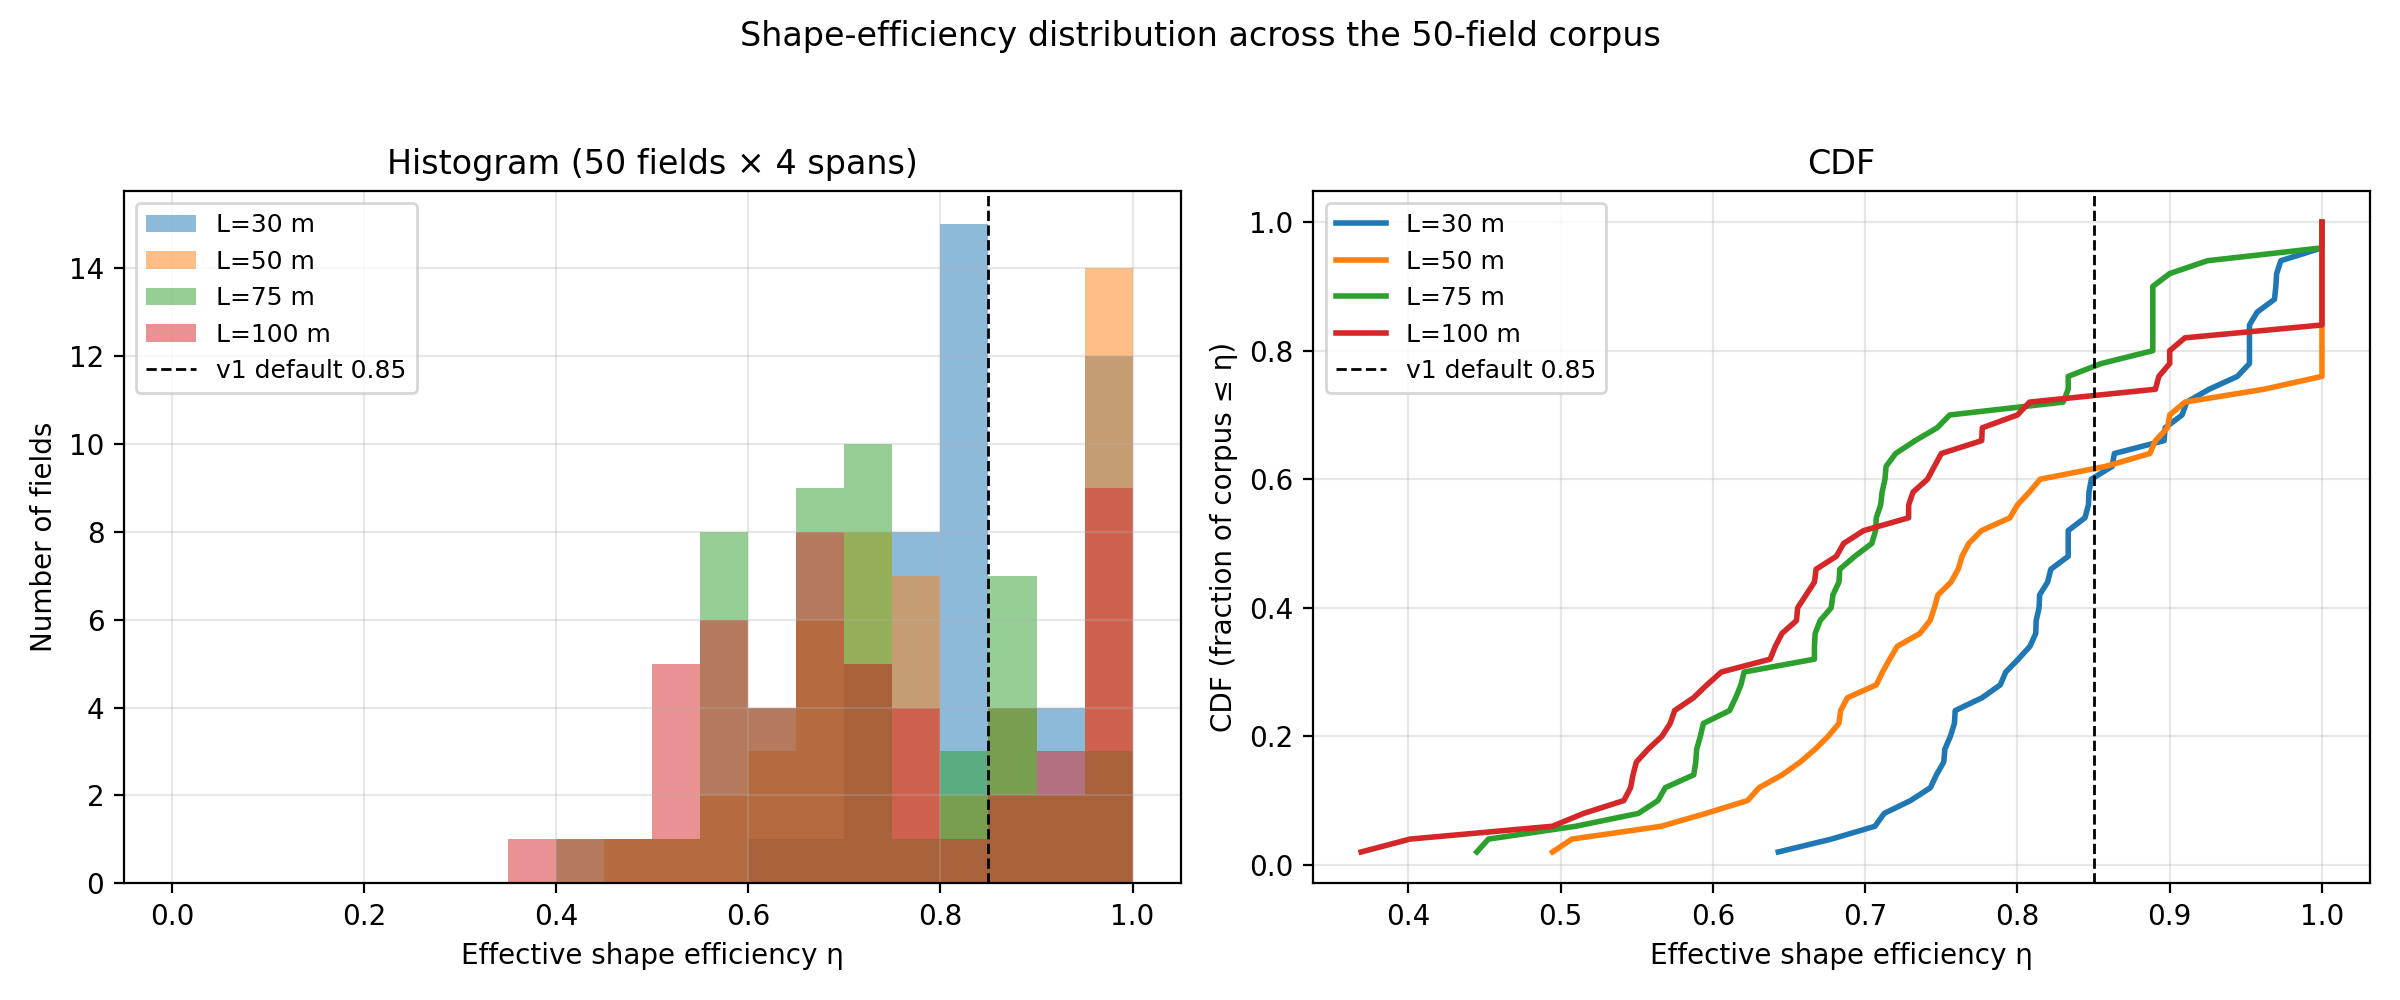
\includegraphics[width=0.85\linewidth]{F9_shape_efficiency_distribution}
\caption{Distribution of best-orientation shape efficiency $\eta$ across the 50-field corpus, by class.}
\label{fig:f9}
\end{figure}

\begin{table}[H]
\centering\small
\caption{Best-orientation shape efficiency $\eta$ by field class at $L = \SI{50}{\meter}$.}\label{tab:eta-classes}
\begin{tabular}{lrrrr}
\toprule
Shape class       & $n$ & Median $\eta$ & P10  & P90 \\
\midrule
rectangle         & 10  & 1.000  & 1.000 & 1.000 \\
L\_shape          & 10  & 0.905  & 0.847 & 1.000 \\
real\_shape       &  5  & 0.800  & 0.776 & 0.862 \\
irregular\_convex & 10  & 0.702  & 0.624 & 0.769 \\
irregular\_concave& 15  & 0.684  & 0.543 & 0.759 \\
\bottomrule
\end{tabular}
\end{table}

\subsubsection{Findings and interpretation}\label{sec:layout-findings}

\textbf{Corpus headline.} The corpus median best-orientation $\eta$ at $L = \SI{50}{\meter}$ is \textbf{0.77}, almost a full \textbf{0.08 point below the 0.85 default} that flat feasibility studies typically use. Carrying that 0.08-point gap through the throughput model translates into roughly a 10\,\% throughput reduction on a like-for-like basis: a feasibility study that assumes \texttt{shape\_efficiency = 0.85} on the same corpus is implicitly over-claiming throughput by about one decare per day on the codesigned reference. Shape geometry is therefore not a second-order effect that can be folded into a constant; it is a first-order determinant of headline daily area, and it has to be sampled across a corpus rather than picked once.

\textbf{Class structure.} The class breakdown in \cref{tab:eta-classes} explains where the gap comes from and is the more useful number than the corpus median:
\begin{itemize}[leftmargin=1.6em,itemsep=0.15em]
    \item \textbf{Rectangles $\eta = 1.000$ (P10 $=$ P50 $=$ P90).} The strip planner is geometrically lossless on rectangles, which is the right answer: a long edge to anchor against and a short edge to step across is exactly the geometry the cable architecture was designed for. This sets a hard ceiling on what the architecture can deliver.
    \item \textbf{L-shapes $\eta = 0.905$.} A single concave corner costs the planner about 10 percentage points of efficiency, because the strips straddling the missing corner each pay a full Anchor placement to cover a sub-strip-length of polygon. The penalty is bounded and predictable.
    \item \textbf{Real shapes $\eta = 0.800$.} The five hand-traced outlines (river-edge strip, road frontage, pentagon, quarter circle, two-lobe peanut) come in tighter than irregular convex polygons because the irregularity sits along one axis and the planner's orientation sweep can usually find an alignment that suppresses it.
    \item \textbf{Irregular convex $\eta = 0.702$ and irregular concave $\eta = 0.684$.} The two ``hard'' classes converge --- once a polygon is irregular enough that no orientation aligns the strips with a long free edge, adding interior obstacles and concave notches on top of that costs only a further $\sim$2 points. The dominant penalty is failing to find a clean strip axis, not the obstacles themselves.
\end{itemize}
The headline reading is that the architecture is \textbf{geometry-sensitive but not geometry-fragile}: the median field in a deliberately adversarial corpus still recovers 77\,\% of its theoretical throughput. The 12-orientation sweep in \cref{eq:eta-shape} matters here --- a fixed-orientation planner would lose another 5--10 points on the irregular classes, because the optimal sweep direction varies field by field.

\textbf{What CableTract's shape sensitivity tells you about siting.} The class spread implies that shape efficiency is a \emph{site-selection variable}, not a residual error term. A farmer choosing between two candidate parcels of the same area should prefer the rectangular one, and the manuscript carries this through into the operating envelope of \cref{sec:envelope}: the model rewards rectangular plots in solar-rich climates and penalises concave plots in temperate ones.

\textbf{Time budget --- the operation is operation-bound, not setup-bound.} \Cref{fig:f10} plots three example strip plans. \Cref{fig:f11} plots the daily time budget on a 5-field 21-ha synthetic farm: \textbf{operating time ${\approx}\SI{37.6}{\hour}$, setup ${\approx}\SI{3.85}{\hour}$, inter-field travel ${\approx}\SI{0.22}{\hour}$.} Operating dominates setup by roughly $10\times$, and dominates inter-field travel by more than $150\times$. This is the most important number in this section, because it overturns the obvious intuition that ``cable architectures must be setup-bound''. They are not, at least not on a small-farm corpus: \emph{the binding cost on a CableTract day is the time spent actually pulling the implement, not the time spent moving the Anchor between fields.} Two consequences follow from this directly:
\begin{itemize}[leftmargin=1.6em,itemsep=0.15em]
    \item Engineering effort spent on faster Anchor placement (hydraulic auto-driving, drone-assisted alignment, pre-staged anchor pads) hits a ceiling at the 9\,\% setup share. Even a perfect zero-setup-time variant of the architecture would only buy back $\sim$10\,\% throughput.
    \item Engineering effort spent on faster operation --- wider strips, higher operating speed within the soil-draft envelope, lower drivetrain losses --- has a direct $1{:}1$ payoff because it acts on the dominant 90\,\% slice. The codesign decision in \cref{sec:codesign} to widen the strip and slow the carriage is therefore aimed at the right slice.
\end{itemize}
This is the geometric reason the codesign argument in \cref{sec:codesign} works at all: given that the operating-time slice dominates, slowing the carriage to suppress the $v^2$ term in \cref{eq:d497} buys energy without losing time, because the time gap is filled by operation savings rather than setup overheads. A different architecture --- say, a system with one-minute setup but \SI{8}{\kilo\meter\per\hour} operation --- would inherit the opposite trade-off and would fail for the opposite reason.

\begin{figure}[H]
\centering
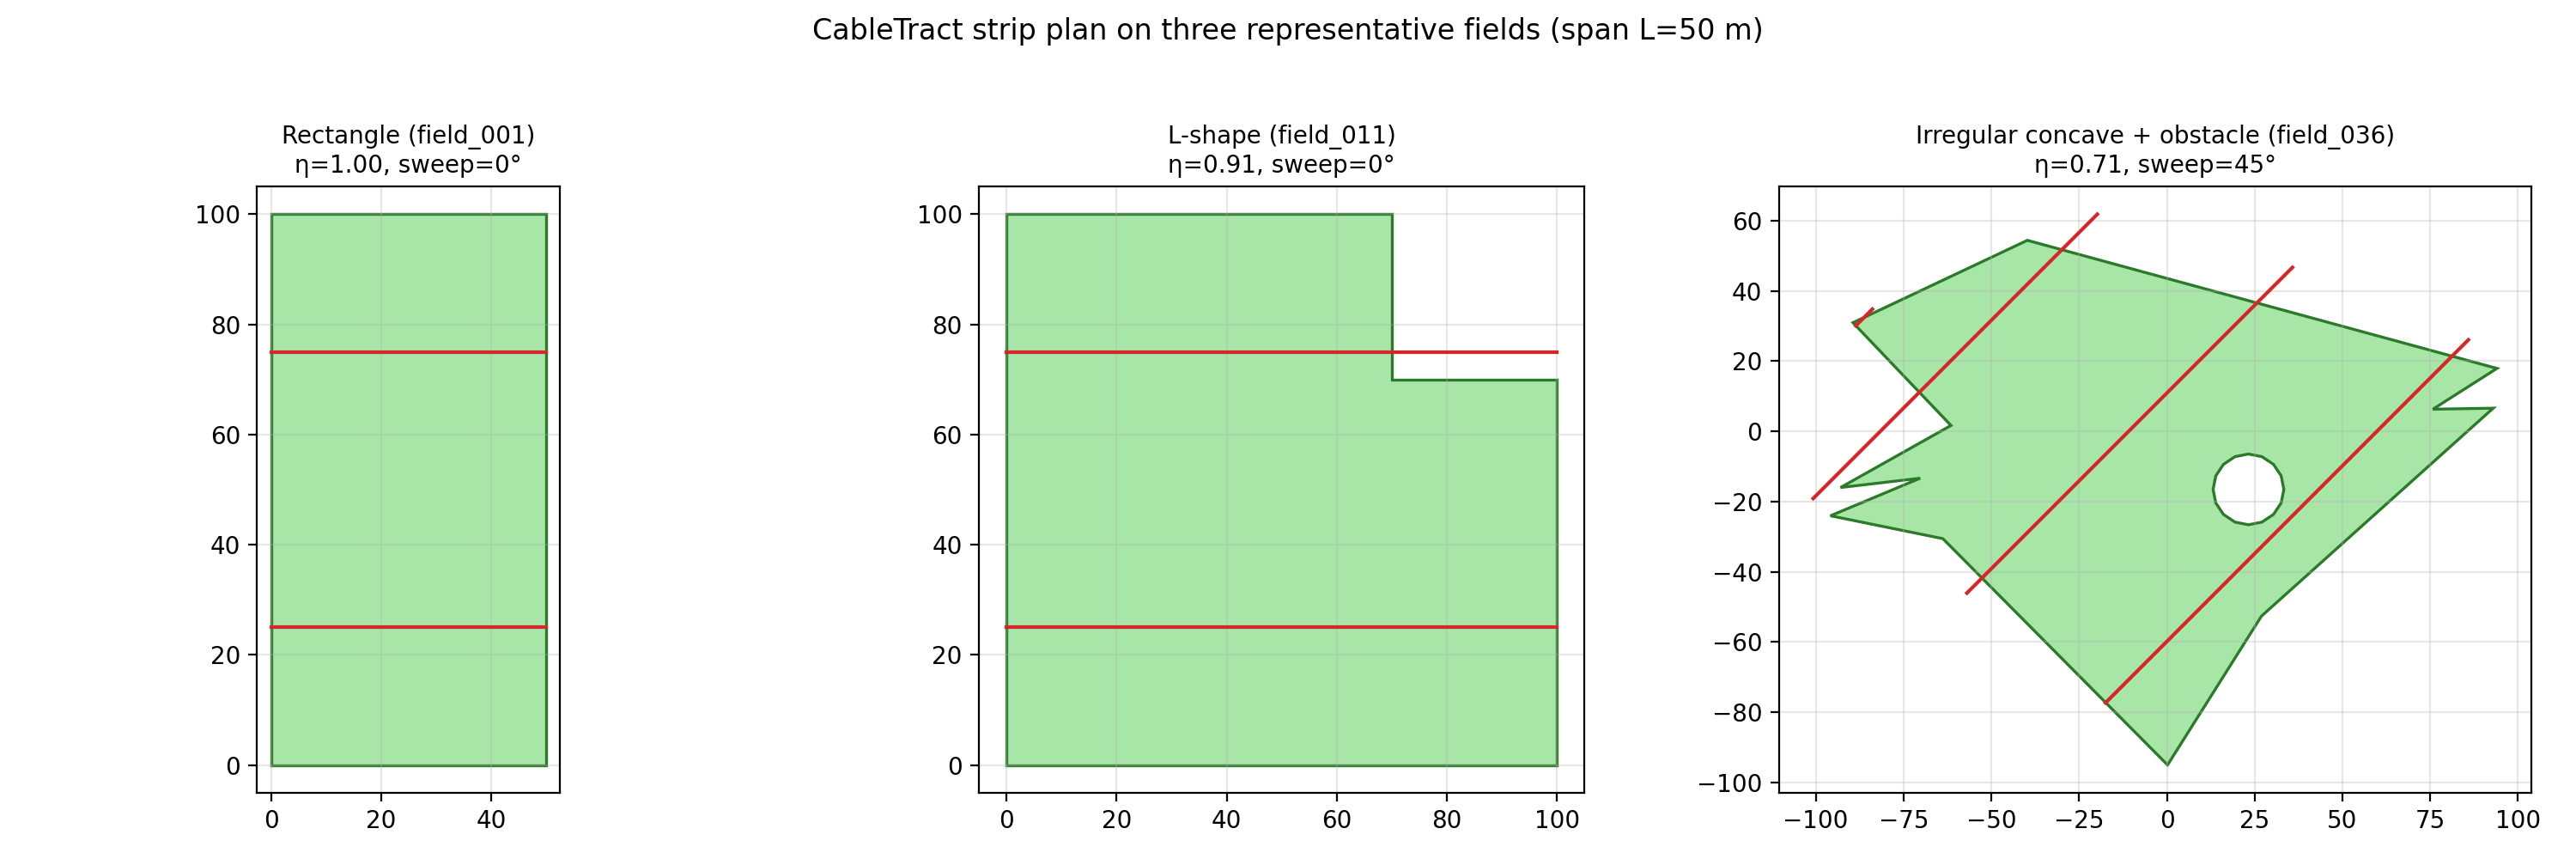
\includegraphics[width=0.95\linewidth]{F10_strip_plans}
\caption{Strip-decomposition plans on three example field shapes (rectangle, L-shape, irregular-concave). Red lines show the per-strip cable lay; green polygons are the field outlines.}
\label{fig:f10}
\end{figure}

\begin{figure}[H]
\centering
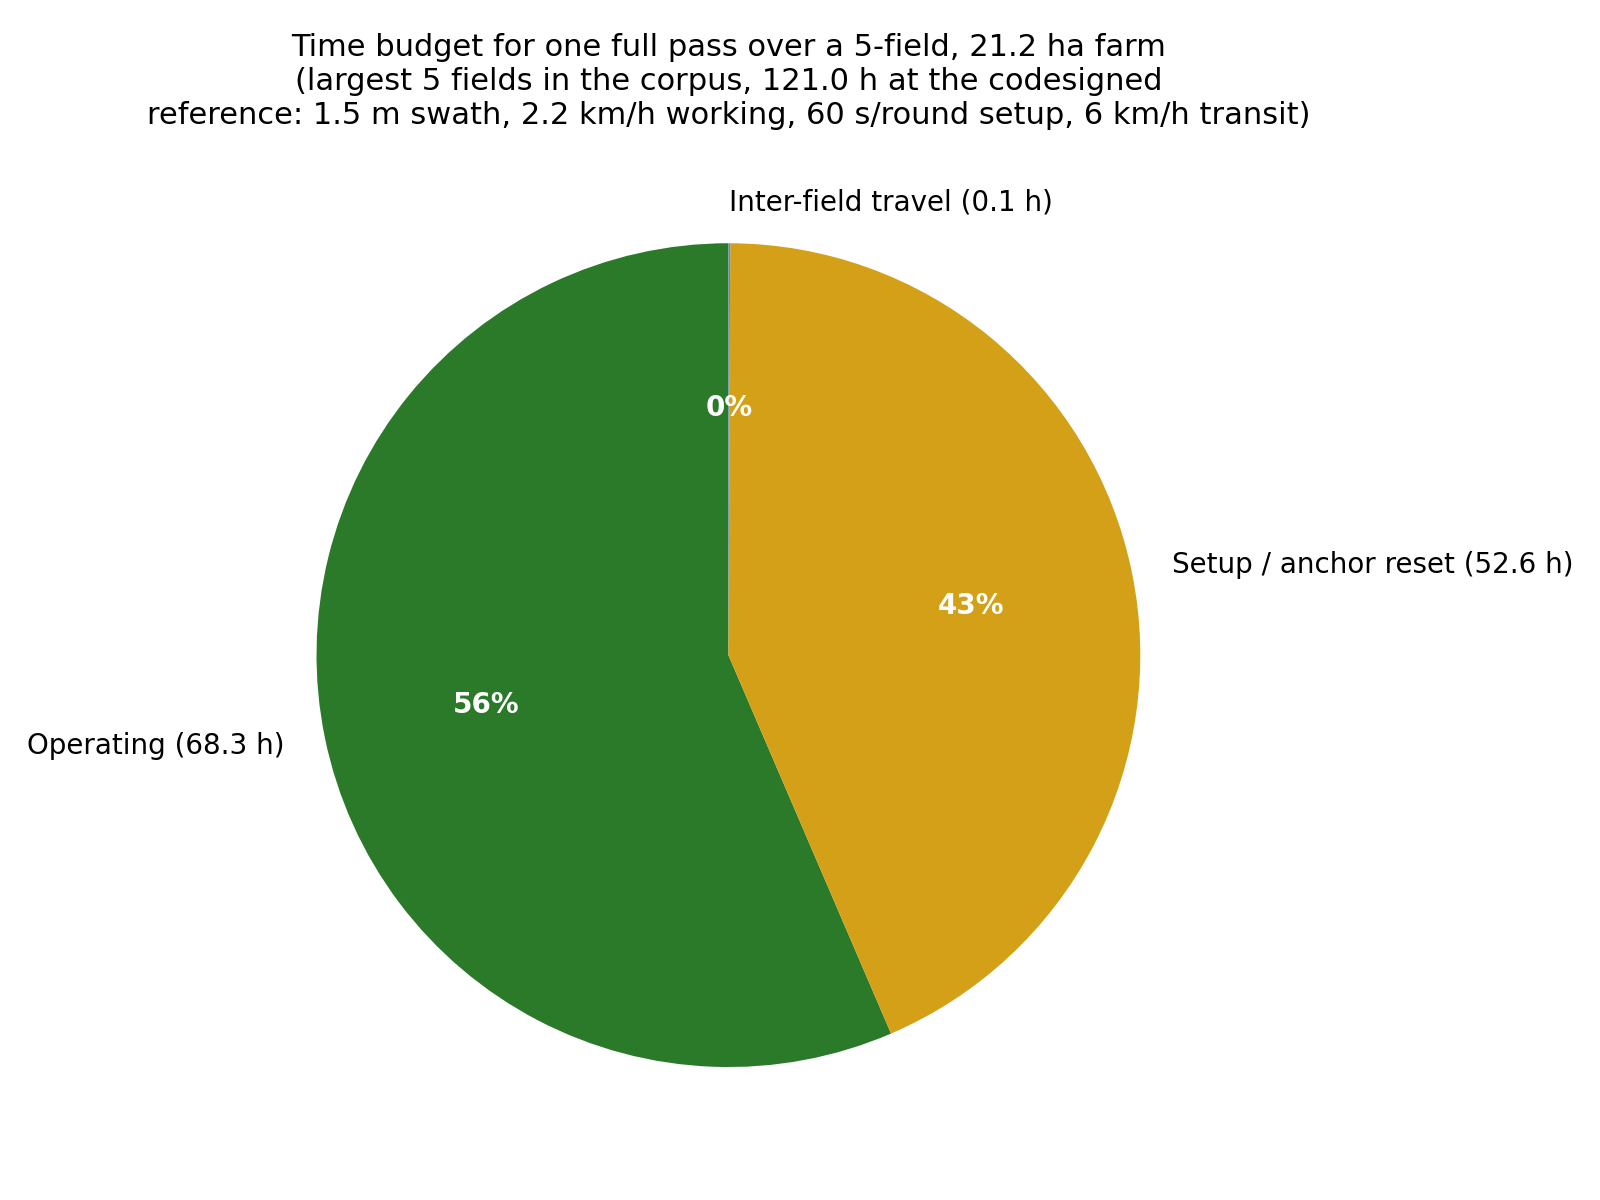
\includegraphics[width=0.65\linewidth]{F11_time_budget}
\caption{Time budget to fully cover a 5-field 21-ha synthetic farm at the codesigned reference, broken into operation, setup, and inter-field travel. Operating time dominates setup by ${\sim}10\times$ and inter-field travel by ${>}150\times$, so the system is operation-bound, not setup-bound.}
\label{fig:f11}
\end{figure}

\subsection{Compaction model}\label{sec:compaction}

The compaction story rests on the in-field footprint of CableTract being the \SI{250}{\kilogram} carriage rather than a multi-tonne tractor body. Turning that architectural statement into a defensible per-hectare reduction requires two ingredients: reference contact pressures for an \SI{80}{hp} \gls{wd} tractor drawn from the soil-mechanics literature, and a comparable per-pass compacted-area accounting for the carriage's narrow rollers. \Cref{sec:vehicle-ref,sec:compaction-metrics} provide both.

\subsubsection{Vehicle reference parameters}\label{sec:vehicle-ref}

\begin{table}[H]
\centering\small
\caption{Reference contact pressures for the tractor and the carriage. The reference tractor sits in the \SIrange{100}{250}{\kilo\pascal} band reported by Keller and Lamand\'e (2010)~\cite{keller2010compaction}; the carriage rollers are wide enough to keep per-patch pressure below \SI{50}{\kilo\pascal}. The static stress-propagation kernel used to convert these contact pressures into the bulk-density depth profiles of \cref{fig:f12} follows S\"ohne (1953)~\cite{sohne1953druck}.}\label{tab:vehicle-pressures}
\begin{tabular}{lcrrr}
\toprule
Vehicle & Wheels & Total mass & Mean $p$ (kPa) & Max $p$ (kPa) \\
\midrule
Reference \SI{80}{hp} \gls{wd} tractor & 4 (front+rear) & ${\approx}\SI{4}{\tonne}$  & \textbf{143} & \textbf{150} \\
CableTract carriage                    & 2 wide rollers & ${\approx}\SI{250}{\kilogram}$ & \textbf{31}  & \textbf{31}  \\
\bottomrule
\end{tabular}
\end{table}

\subsubsection{Compacted-area and contact-energy metrics}\label{sec:compaction-metrics}

For each (vehicle, field) pair we compute four scalar compaction metrics:

\begin{itemize}[leftmargin=1.6em,itemsep=0.1em]
    \item \textbf{Compacted area (\si{\meter\squared}).} For the tractor: polygon area $\times$ per-pass coverage fraction; for the carriage: strip-midline path $\times$ roller width $\times$ pass count.
    \item \textbf{Compacted area fraction.} Compacted area / (polygon area $\times$ pass count).
    \item \textbf{Mean pressure (\si{\kilo\pascal}).} Load-weighted mean of all wheel contact pressures.
    \item \textbf{Contact-energy index.} $\sum p^{2} \cdot A_{\text{patch}} \cdot \text{pass\_count}$, in (\si{\kilo\pascal\squared.\meter\squared}). Pressure squared because soil-stress propagation is roughly quadratic in surface load.
\end{itemize}

A 4-pass cropping season is the default.

\subsubsection{Compaction map}\label{sec:f12}

\begin{figure}[H]
\centering
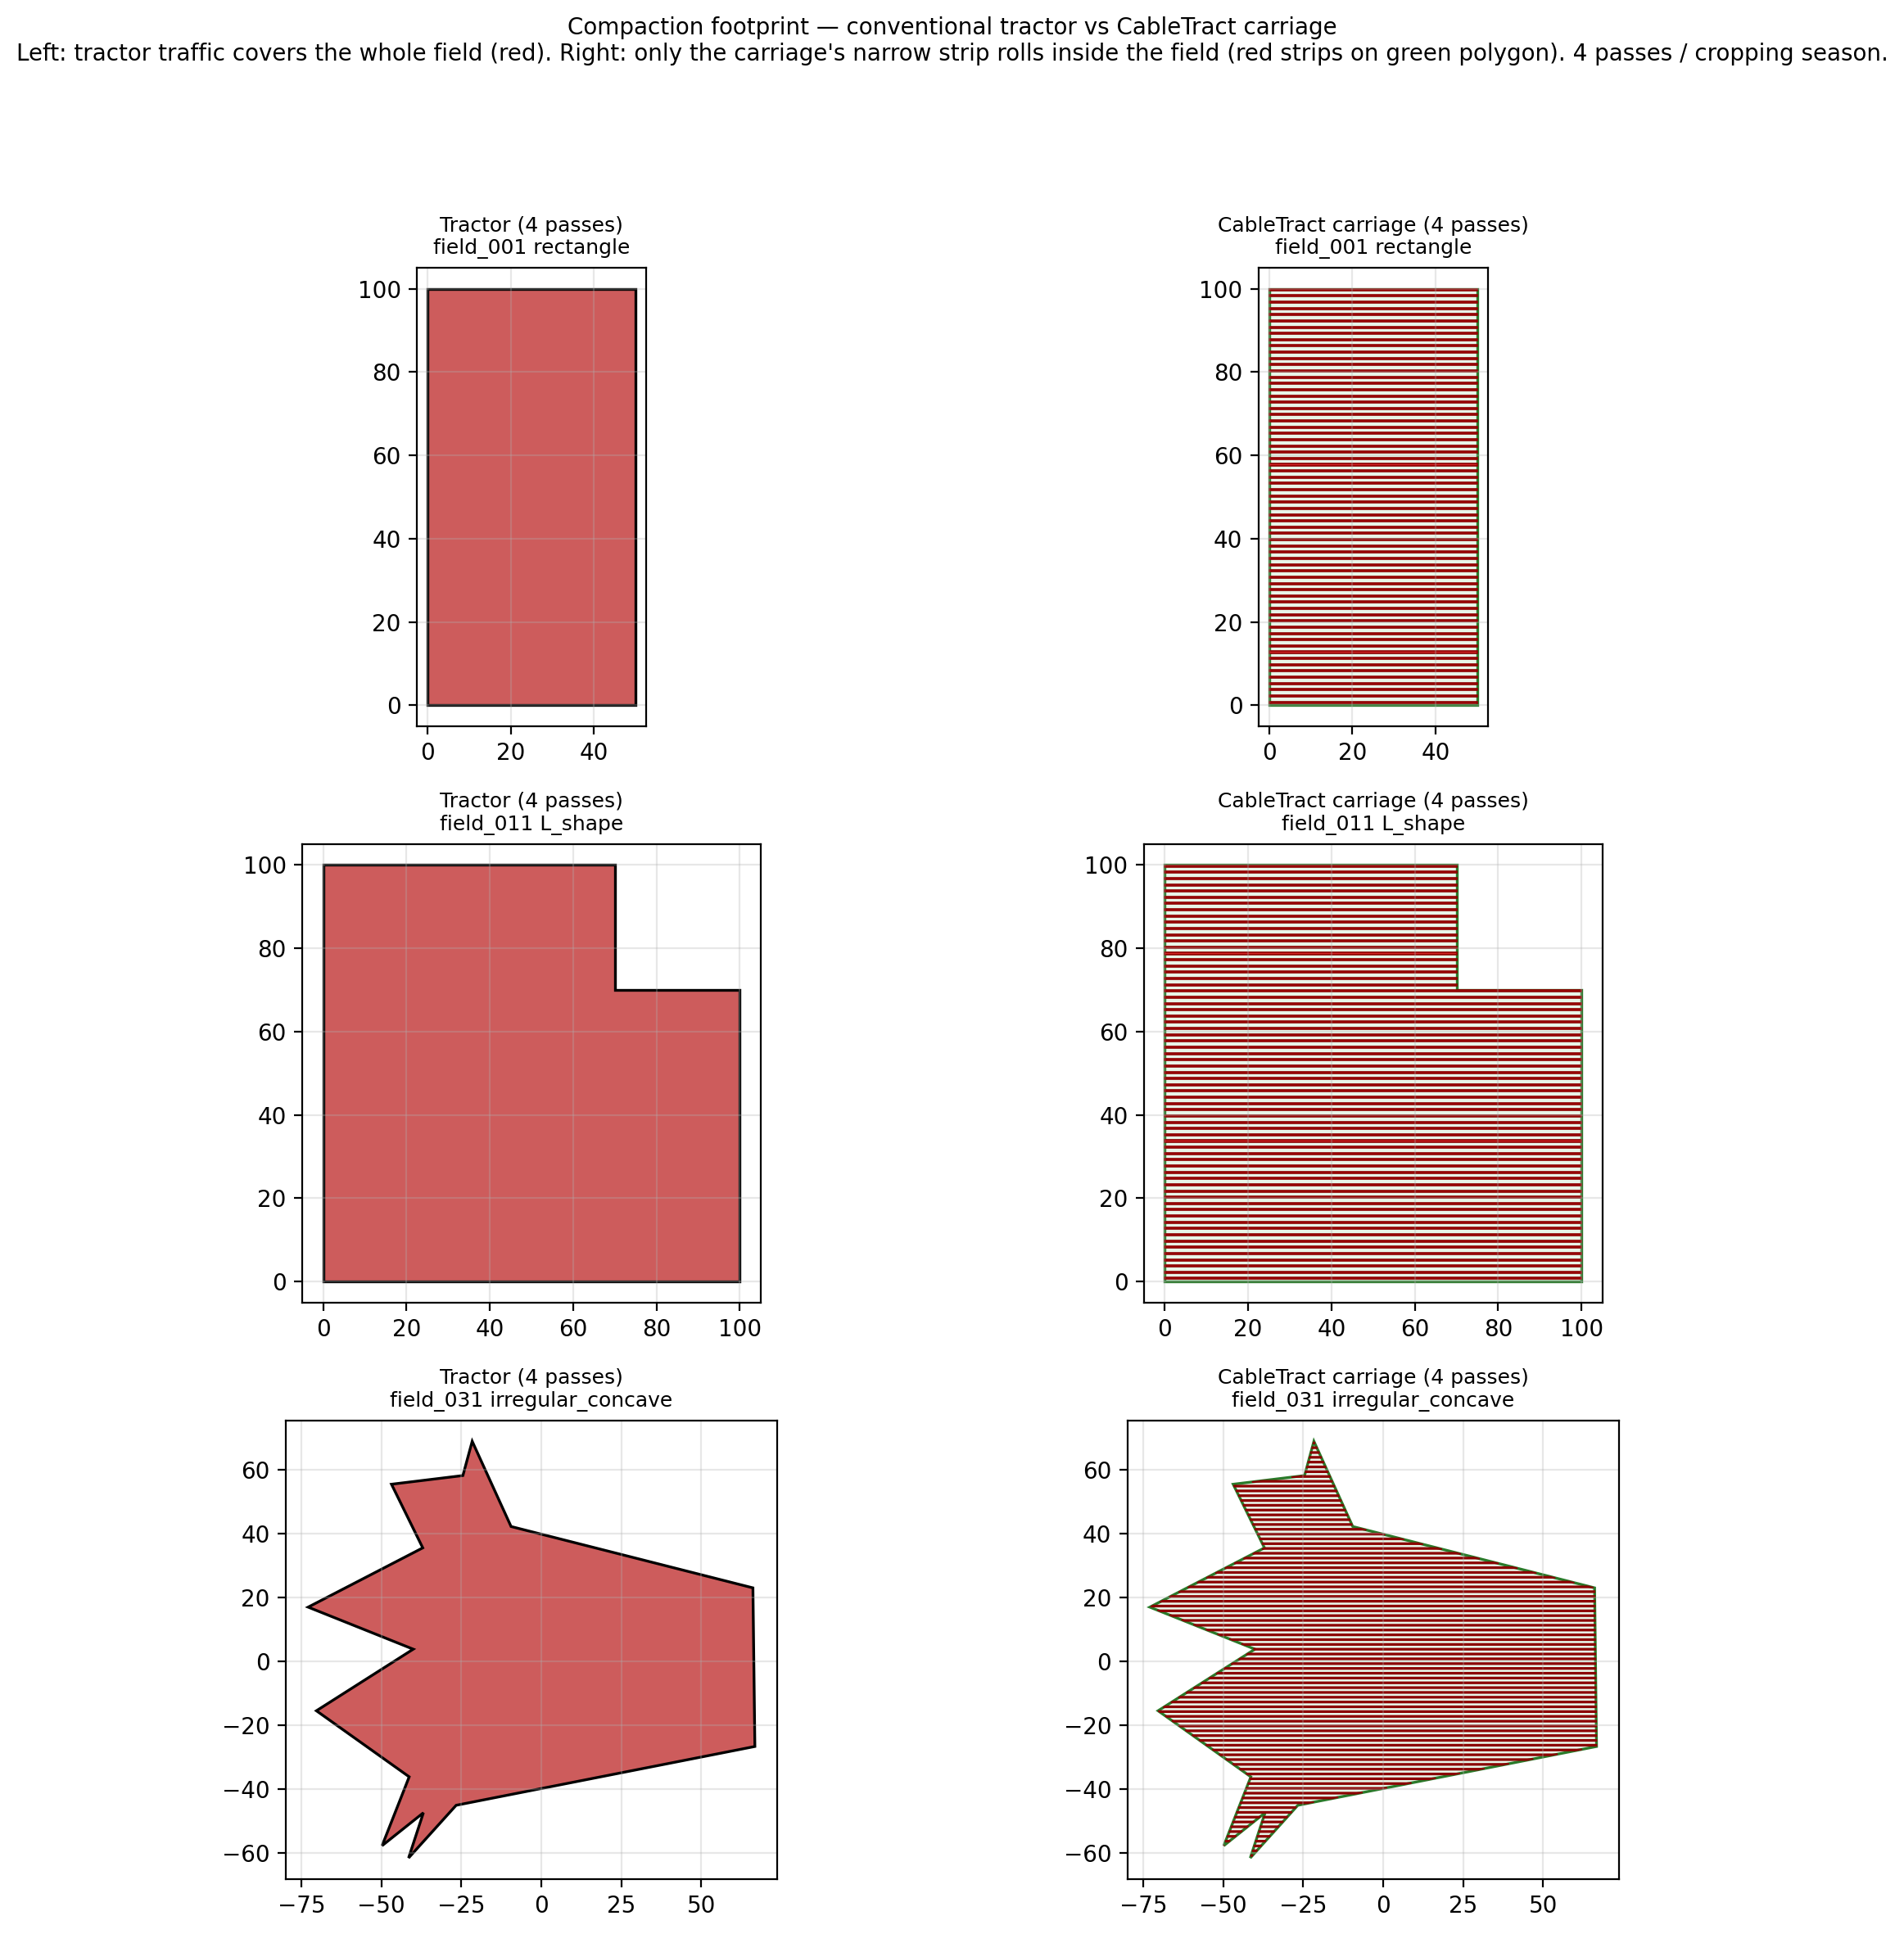
\includegraphics[width=0.95\linewidth]{F12_compaction_map}
\caption{Compaction comparison on three field classes (rectangle, L-shape, irregular-concave). Tractor coverage paths in red, carriage strip-midline paths in green. The carriage's compacted area is essentially an L-shaped frame around the strip pattern; the tractor's covers the entire field on every pass.}
\label{fig:f12}
\end{figure}

\begin{table}[H]
\centering\small
\caption{Per-field compaction summary. Area reduction is geometric (only the carriage rolls inside the field); the energy index reduction adds a $4.6\times$ pressure ratio squared.}\label{tab:compaction}
\resizebox{\textwidth}{!}{%
\begin{tabular}{lllrrrr}
\toprule
Field & Class & & Tractor compacted & Carriage compacted & Area reduction & Energy index reduction \\
\midrule
field\_001 & rectangle         & & 50\,\% & 0.8\,\% & 98\,\% & $73\times$ \\
field\_011 & L\_shape          & & 50\,\% & 0.9\,\% & 98\,\% & $73\times$ \\
field\_031 & irregular\_concave& & 50\,\% & 1.4\,\% & 97\,\% & $73\times$ \\
\bottomrule
\end{tabular}%
}
\end{table}

\textbf{CableTract reduces compacted \emph{area} by 97--98\,\%} on every field shape in the corpus, because only the lightweight carriage rolls inside the field while the heavy MU and Anchor stay on the headland.

\textbf{The contact-energy index drops by ${\approx}\,73\times$} on every field, because the carriage's mean pressure is $4.6\times$ lower than the tractor's, and the energy integrand depends on $p^{2}$.

These two numbers --- area reduction near 100\,\% and contact-energy reduction near two orders of magnitude --- are the strongest single quantitative argument the paper makes for the cable architecture, and they are both defensible from open published static contact-pressure values without any dynamic \gls{fem} calibration. \Cref{sec:limitations} notes that the model deliberately ignores headland turns, dynamic load transfer, and multi-pass cumulative deformation; including those would \emph{strengthen} the comparison by adding compaction to the tractor side.

\subsection{Uncertainty quantification and global sensitivity}\label{sec:uq}

Every number in \cref{sec:physics,sec:soil,sec:energy,sec:economics,sec:layout,sec:compaction} depends on parameters whose values are known to within published uncertainty bands rather than exactly. A defensible feasibility envelope must therefore answer two questions: given the joint uncertainty in 20 parameters, what is the \textbf{P10--P90 envelope} of the headline outputs, and which parameters carry the most variance --- in particular, is any single parameter still dominant after the \cref{sec:drivetrain} decomposition of the lumped drivetrain efficiency? We answer the first with a 1\,000-sample Monte Carlo and the second with a Sobol global sensitivity decomposition~\cite{sobol2001indices,saltelli2008primer} computed via \gls{salib}~\cite{herman2017salib,iwanaga2022salib}.

\subsubsection{Parameter problem}\label{sec:uq-problem}

The uncertainty problem is defined over 20 parameters drawn from physically defensible bands with uniform marginals. Examples:

\begin{itemize}[leftmargin=1.6em,itemsep=0.1em]
    \item Lumped drivetrain efficiency $\in [0.35, 0.65]$ --- covers the manufacturer datasheet range for industrial \gls{pmsm}/gearbox/drum/cable chains after the \cref{sec:drivetrain} decomposition.
    \item Draft load $\in [\SI{1500}{\newton}, \SI{4500}{\newton}]$ --- spans the codesigned-library P10--P90 envelope from \cref{sec:soil}.
    \item Shape efficiency $\in [0.55, 1.00]$ --- covers the entire field-corpus range from \cref{fig:f9}.
    \item PV area $\in [\SI{10}{\meter\squared}, \SI{30}{\meter\squared}]$ and battery capacity $\in [\SI{5}{\kWh}, \SI{25}{\kWh}]$ --- spans the design envelope of \cref{fig:f8}.
\end{itemize}

These bands are deliberately wider than typical sensitivity studies on energy systems, so the resulting Sobol decomposition is hard to fudge.

\subsubsection{Monte Carlo}\label{sec:mc}

We draw $n = 1000$ samples from the joint distribution and evaluate the full simulator on each. Doubling the sample size to 2000 shifts \gls{p50} by less than 1\,\% and \gls{p10}/\gls{p90} by less than 3\,\%, so 1\,000 samples are sufficient. \Cref{fig:f15} plots the resulting throughput envelope versus draft load, with the codesigned reference (\SI{1800}{\newton}, \SI{11.5}{decares\per day}) overlaid as a green star. The star sits below the \gls{p50} line ($\sim$\SI{13.7}{decares\per day} at the same draft) but well inside the P10--P90 envelope, which is the expected behaviour: the deterministic codesigned reference uses pessimistic-leaning defaults on several uncertain parameters (drivetrain efficiency chain, soil moisture, headland turning), so it should land in the lower half of the joint distribution rather than at its centre. The Monte Carlo run is a check on robustness, not a re-derivation of the codesigned point.

\begin{figure}[H]
\centering

\includegraphics[width=0.85\linewidth]{F15_mc_throughput_envelope}
\caption{Monte Carlo throughput envelope versus draft load (1\,000 samples). Codesigned reference overlaid as a green star.}
\label{fig:f15}
\end{figure}

\subsubsection{Global sensitivity}\label{sec:sobol}

First-order (\gls{sobol1}) and total-order (\gls{sobolt}) Sobol indices~\cite{sobol2001indices} are estimated with the Saltelli sampler~\cite{saltelli2008primer,herman2017salib} at $n_{\text{base}} = 256$, giving $256 \times (2 \times 20 + 2) = 10\,752$ simulator evaluations per Sobol pass. The four targets are daily off-grid throughput, energy per decare, payback versus diesel, and surplus power.

\begin{figure}[H]
\centering

\includegraphics[width=0.95\linewidth]{F13_sobol_bars}
\caption{Sobol \gls{sobol1} and \gls{sobolt} indices for the top-15 parameters across the four headline outputs. After the \cref{sec:drivetrain} decomposition of the lumped drivetrain efficiency, no single parameter accounts for more than 20\,\% of the variance in throughput.}
\label{fig:f13}
\end{figure}

\textbf{After the decomposition of the lumped drivetrain efficiency, the variance is diffuse.} For daily throughput, the five largest contributors --- daily solar hours, draft load, PV area, strip width, and irradiance intensity --- each sit in the band $\gls{sobolt} \in [0.13, 0.20]$. No single parameter accounts for more than 20\,\% of the variance, and the top five together explain ${\approx}\,80\%$. The codesigned reference is not a hand-tuned local optimum sitting on top of one undefended fudge factor; it is robust to the full joint uncertainty in the 20 inputs.

\subsubsection{Tornado on NPV}\label{sec:tornado}

\textbf{What this analysis answers.} The Sobol decomposition in \cref{fig:f13} answers the question ``where does throughput \emph{variance} come from when 20 inputs vary jointly?''. That is the right question for engineering design, but it is not the right question for a sceptical financial reviewer, who wants to know something more direct: \emph{which single inputs, varied across realistic bounds, can flip the financial story --- and which ones cannot?} A tornado analysis is the standard tool for that question. Each parameter is varied one at a time between a low and a high bound while every other parameter is held at its codesigned reference, and the resulting two \gls{npv} values are recorded. The bar for that parameter is then drawn from $\mathrm{NPV}_{\mathrm{lo}}$ to $\mathrm{NPV}_{\mathrm{hi}}$, and the parameters are sorted by total swing $|\mathrm{NPV}_{\mathrm{hi}} - \mathrm{NPV}_{\mathrm{lo}}|$ from largest to smallest. The shape of the resulting plot --- wide bars on top, narrow bars on the bottom --- is what gives the tornado its name.

\textbf{The protocol.} The \gls{npv} reported here is \gls{npv} \emph{against a diesel tractor baseline} at the codesigned operating point (\SI{25}{\hectare\per\year}, 8\,\% discount rate, 15-year horizon, year-8 battery replacement, 4\,\%/yr maintenance, all from \cref{tab:econparams}). A positive number means CableTract beats the diesel tractor by that many euros over the project horizon in present-value terms; a negative number means diesel wins. The baseline at the codesigned reference is \textbf{€70,300}, marked as the dashed vertical line in \cref{fig:f14}. (This is a different framing from \cref{tab:npv-farmsize}, which reports the much smaller \SI{+3978}{\EUR} \gls{npv} delta against a like-for-like used diesel tractor; the tornado uses the gross-savings frame so each parameter swing is read as a fraction of the full project value rather than of the marginal capex difference.) Each green bar shows where \gls{npv} moves when the parameter is pushed to the side that \emph{helps} CableTract; each red bar shows the side that \emph{hurts} it. The 20 inputs from \cref{sec:uq-problem} are tested; the top 10 by swing are plotted.

\begin{figure}[H]
\centering

\includegraphics[width=0.85\linewidth]{F14_tornado_npv}
\caption{Tornado plot of one-at-a-time \gls{npv}-vs-diesel elasticities at the codesigned reference (\SI{25}{\hectare\per\year}, 8\,\% discount, 15-yr horizon). Baseline NPV €70,300 in the gross-savings frame (see body text for the reconciliation with \cref{tab:npv-farmsize}). Each bar varies one parameter across its realistic range (\cref{sec:uq-problem}) while all others are held at the codesigned default. Green = the side that helps CableTract; red = the side that hurts it. Sorted top to bottom by total swing.}
\label{fig:f14}
\end{figure}

\textbf{How to read the figure --- the three tiers.} The top 10 swings cluster cleanly into three tiers, and the tier structure is the most important thing to take away from \cref{fig:f14}.

\begin{itemize}[leftmargin=1.6em,itemsep=0.2em]
    \item \textbf{Tier 1 --- the four big swings (€46--54k).} \texttt{solar\_area\_m2} (\SI{10}{\meter\squared}~$\to$~\SI{30}{\meter\squared}), \texttt{fuel\_price\_usd\_per\_l} (\SI{0.8}{\EUR\per\litre}~$\to$~\SI{1.8}{\EUR\per\litre}), \texttt{fuel\_l\_per\_decare} (\SIrange{1}{3}{\litre}), and \texttt{width\_m} (\SIrange{1.5}{3.0}{\meter}). These are the parameters that can shift \gls{npv} by more than half a typical Tier-1 result. \textbf{Three of the four are not under the engineer's control}: PV area is a deployment choice but the other two ``fuel'' parameters describe \emph{the diesel tractor we are competing against}. If diesel becomes cheap or the comparison crop is light enough that a diesel tractor only burns one litre per decare, the financial gap shrinks to ${\approx}\,$€47,000. If diesel becomes expensive or the operation is heavy enough to burn three litres per decare, the gap grows to ${\approx}\,$€93,000. Both outcomes are still solidly positive --- which is the headline finding of the entire tornado.
    \item The \texttt{width\_m} bar is the only one-sided bar in the figure: the codesigned strip width \SI{1.5}{\meter} sits at the \emph{low} end of the tested range, so the green half of the bar (going wider) is the only side that exists. Widening the strip from \SI{1.5}{\meter} to \SI{3.0}{\meter} (without re-paying for the implement) would lift \gls{npv} from €70,300 to €116,726. This is not a free move --- a wider implement costs more and adds draft load --- but it tells us where the next \gls{npv} headroom lives if anyone decides to push the design.
    \item \textbf{Tier 2 --- the resource and drivetrain swings (€27--34k).} \texttt{solar\_power\_W\_m2}, \texttt{draft\_load\_N}, \texttt{solar\_hours\_per\_day}, \texttt{winch\_efficiency}, and \texttt{operating\_days\_per\_year}. These five parameters describe the \emph{climate} (irradiance intensity and daylight) and the \emph{drivetrain} (winch efficiency and the implement-side load). They each shift \gls{npv} by about half a Tier-1 swing. The only one of these that is unambiguously under the engineer's control is \texttt{winch\_efficiency}, and even there the lumped value sits in the middle of the tested 0.35--0.65 range; the worst case (\SI{56400}{\EUR}) is still firmly NPV-positive.
    \item \textbf{Tier 3 --- the small swings (${\leq}\SI{21000}{\EUR}$).} \texttt{shape\_efficiency}, \texttt{implement\_weight\_N}, \texttt{cost\_cabletract\_usd}, and the wind / battery / span / weight / setup parameters that fall off the bottom of the chart entirely. Note in particular that \texttt{cost\_cabletract\_usd} (the \gls{capex} of the system itself) is only Tier 3 with a swing of \SI{16100}{\EUR}: even at the high end of the tested capex range (\SI{22000}{\EUR}, vs the codesigned \SI{16000}{\EUR}), CableTract still beats diesel by \SI{56200}{\EUR}. This is the consequence of the capex-parity decision in \cref{tab:econparams}: capex hurdles are not where the binding constraint sits, and that is why the parameter that obsesses most clean-energy-hardware feasibility studies sits this far down.
\end{itemize}

\textbf{Headline finding --- the result is robust because it is exogenous-led.} The dashed baseline line at \SI{70300}{\EUR} sits inside the green half of every Tier-1 and Tier-2 bar. \emph{No single parameter, taken to either end of its plausible range, can flip the sign of NPV vs diesel at the codesigned operating point.} The most pessimistic single-parameter swing in the entire tornado is \texttt{draft\_load\_N} pushed to \SI{4500}{\newton} (the heaviest moldboard plowing case), which drops \gls{npv} to \SI{46100}{\EUR} --- still solidly positive. There is no parameter in the tornado that can take the bar across zero on its own.

\textbf{What is and is not under our control.} Of the top three swings, the engineer controls only \texttt{solar\_area\_m2} --- which is a deployment knob, not an architectural choice. The other two top swings (\texttt{fuel\_price\_usd\_per\_l}, \texttt{fuel\_l\_per\_decare}) describe \emph{the world we are competing against}, not the world we are building. This is good news for the architecture: it means the financial story is driven by the macro environment of agricultural diesel rather than by any single fudge factor inside the model. It also means the financial story improves over time --- agricultural diesel prices have a strong upward trend, and crop intensification has a strong upward trend on litres per decare, both of which push CableTract's \gls{npv} into the green half of the Tier-1 bars.

\textbf{What this rules out.} A common failure mode in feasibility papers is that a single parameter (battery price, capex, drivetrain efficiency, ``magic fudge factor'') turns out to be the load-bearing assumption that drives the entire result. \cref{fig:f14} rules this failure mode out for the codesigned reference: every Tier-1 swing is exogenous, every Tier-2 swing leaves the result solidly positive, and the design parameter (\texttt{cost\_cabletract\_usd}) that the model has the most leverage to be wrong about sits in Tier 3 with no sign-flipping power. Combined with the diffuse Sobol decomposition in \cref{fig:f13}, this is the key robustness statement of the paper.

\subsubsection{NPV vs farm size}\label{sec:npv-farmsize}

\Cref{fig:f16} sweeps the discounted-cash-flow chain over six farm sizes (1, 5, 10, 25, 50, 100 ha/yr) at three discount rates (5/8/12\,\%). At the codesigned reference (\cref{tab:npv-farmsize}):

\begin{table}[H]
\centering\small
\caption{NPV vs diesel and discounted payback at six farm sizes and three discount rates. Bold row is the codesigned reference (\SI{25}{\hectare\per\year}, 8\,\%).}\label{tab:npv-farmsize}
\resizebox{\textwidth}{!}{%
\begin{tabular}{rrrrr}
\toprule
Farm size (\si{\hectare\per\year}) & NPV @ 5\,\% (\si{\EUR}) & NPV @ 8\,\% (\si{\EUR}) & NPV @ 12\,\% (\si{\EUR}) & Payback @ 8\,\% (\si{\year}) \\
\midrule
1   & +686    & +527    & +392    & 1.85 \\
5   & +1\,383  & +1\,102  & +849    & 1.54 \\
10  & +2\,255  & +1\,821  & +1\,421  & 1.26 \\
\textbf{25}  & \textbf{+4\,871}  & \textbf{+3\,978}  & \textbf{+3\,138}  & \textbf{0.82} \\
50  & +9\,230  & +7\,573  & +5\,998  & 0.53 \\
100 & +17\,949 & +14\,763 & +11\,719 & 0.31 \\
\bottomrule
\end{tabular}%
}
\end{table}

\begin{figure}[H]
\centering

\includegraphics[width=0.85\linewidth]{F16_npv_vs_farm_size}
\caption{\gls{npv} vs diesel as a function of farm size at three discount rates. \gls{npv} is positive across the entire \SIrange{1}{100}{\hectare\per\year} sweep at every discount rate.}
\label{fig:f16}
\end{figure}

\textbf{NPV is positive across the entire (\SIrange{1}{100}{\hectare}) sweep at all three discount rates.} This is the central economic finding of the paper, and it is the \emph{consequence of co-design}: at \gls{capex} parity with a used diesel tractor (\SI{35570}{\EUR} vs \SI{35000}{\EUR}), every euro saved on diesel is gross savings, and the discounted-payback line is well inside the project horizon at every farm size we test.

\begin{figure}[H]
\centering

\includegraphics[width=0.85\linewidth]{F17_lca_co2}
\caption{Lifecycle CO\textsubscript{2} per hectare-year for CableTract, the diesel reference tractor, and a Monarch-class electric tractor (stacked: embodied + fuel/grid). CableTract delivers a $2.2\times$ improvement that does not depend on grid decarbonisation.}
\label{fig:f17}
\end{figure}

\subsection{Architectural variants}\label{sec:ml}

\subsubsection{What this section is for}\label{sec:variants-intro}

Everything up to this point has analysed a single architecture: the codesigned two-module v1, with one stationary Main Unit, one Anchor, a single tensioned cable, and a unidirectional drivetrain. The natural next question is whether that v1 architecture is the only sensible point in the design space, or whether topological modifications --- adding more Main Units, recovering energy on the return leg, changing the cable layout --- materially change the headline numbers. We answer this with a small, deliberately narrow comparison: \textbf{three variants run on the same codesigned parameter set, on the same simulator, so the resulting bars are directly comparable}.

The three variants are chosen so that they probe orthogonal axes of the design space. Each is implemented as a \emph{parameter transformation} on the codesigned reference of \cref{tab:codesigned-params}, fed into the same \texttt{run\_single} routine, with no parallel code path. The result is a clean apples-to-apples comparison rather than three independent feasibility studies that drift apart on definitions.

\begin{itemize}[leftmargin=1.6em,itemsep=0.15em]
    \item \textbf{Codesigned baseline} (\cref{sec:variant-baseline}): the v1 architecture as analysed in \cref{sec:physics,sec:soil,sec:energy,sec:economics}. One Main Unit, one Anchor, one cable, unidirectional drivetrain. This is the reference column of \cref{tab:variants-numbers}.
    \item \textbf{CableTract+, the four-Main-Unit planar cable robot} (\cref{sec:variant-plus}): four corner stations and two simultaneously-pulling cables, so the carriage moves in a 2-D plane between the corners instead of along a 1-D strip. Probes whether \emph{architectural scale} (more modules, no Anchor reset) can outrun the v1.
    \item \textbf{Regenerative return leg} (\cref{sec:variant-regen}): the v1 architecture with four-quadrant motor control on the winch drivetrain so that the unloaded return half of every round recovers kinetic + potential energy back into the battery. Probes whether \emph{drivetrain efficiency engineering} (no new modules, no new mechanics) can outrun the v1.
\end{itemize}

The two ``failed'' variants we considered and explicitly drop from the comparison are: (i) a circular-pulley/oblique-cable variant that lets the Main Unit rotate the cable take-off angle so the Anchor can step laterally without re-anchoring, and (ii) a drone-assisted alignment variant that uses a quadcopter to drop GPS markers between fields. Both reduce setup time, but \cref{sec:layout-findings} already showed that the codesigned reference is \emph{operation-bound, not setup-bound} --- the setup slice is only 9\,\% of the daily time budget --- so any setup-reduction variant has at most a 9\,\% throughput ceiling and is engineering effort spent on the wrong slice. They are listed for completeness in \cref{sec:variants-named} but not part of the variant comparison in \cref{fig:f20}.

\begin{table}[H]
\centering\small
\caption{Architectural variant comparison on the codesigned reference parameter set. All three rows are run on the same \texttt{run\_single} call, with the variant differences applied as parameter transformations on top of \cref{tab:codesigned-params}. CAPEX is the itemised \cref{sec:economics} bill of materials (Main Unit + Anchor + battery + PV + wind + install) in 2024 EUR. ``Simple payback'' is the undiscounted ratio of CAPEX (with sales margin) to annual diesel-fuel savings only --- it is intentionally a more conservative frame than the \cref{sec:economics} discounted payback against the diesel reference, which subtracts a \SI{35000}{\EUR} diesel-tractor capex from the numerator and includes maintenance savings; see the discussion at the end of \cref{sec:variants-discussion} for the reconciliation between the two numbers.}\label{tab:variants-numbers}
\resizebox{\textwidth}{!}{%
\begin{tabular}{lrrrrr}
\toprule
Variant & Throughput (dec/day) & Energy/decare (Wh) & CAPEX (\si{\EUR}) & Simple payback (mo) & Surplus (W) \\
\midrule
\textbf{Codesigned baseline}     & \textbf{11.5} & \textbf{921} & \textbf{35\,570} & \textbf{74.8} & \textbf{291} \\
CableTract+ (4-MU robot)         & 29.3 ($\boldsymbol{2.56\times}$) & 484 ($0.53\times$) & 80\,570 ($2.27\times$) & 89.0 ($1.19\times$) & 896 \\
Regenerative return leg          & 11.8 ($1.03\times$) & 760 ($\boldsymbol{0.83\times}$) & 35\,570 ($\boldsymbol{1.00\times}$) & $\boldsymbol{61.7}$ ($\boldsymbol{0.83\times}$) & 19 \\
\bottomrule
\end{tabular}%
}
\end{table}

\begin{figure}[H]
\centering

\includegraphics[width=0.95\linewidth]{F20_variant_comparison}
\caption{Architectural variant comparison on the codesigned reference parameter set. Codesigned baseline outlined in black. Lower is better for energy, CAPEX, and payback; higher is better for throughput and surplus power.}
\label{fig:f20}
\end{figure}

\subsubsection{Variant 1 --- Codesigned baseline}\label{sec:variant-baseline}

This is the v1 architecture analysed throughout the paper: one Main Unit (PMSM + winch + drum + battery + PV/wind harvester) parked at one headland, one Anchor (helical-pile module that resists the cable reaction) parked at the opposite headland, one steel cable spanning between them at typical span $L = \SI{50}{\meter}$, and a lightweight implement carriage rolling along the cable. The drivetrain is unidirectional --- the motor pulls the carriage outbound under load, and on the return leg the carriage either rolls free (if the field has a slope assist) or is pulled back at idle power. Setup between strips consists of moving the Anchor sideways by one strip width and re-tensioning. The baseline column of \cref{tab:variants-numbers} is the deterministic \texttt{run\_single} output for this architecture at the default codesigned parameter set: \textbf{11.5 decares/day off-grid throughput, 921 Wh/decare energy intensity, \SI{35570}{\EUR} itemised CAPEX (\SI{17500}{\EUR} Main Unit + \SI{7500}{\EUR} Anchor + \SI{3420}{\EUR} \SI{9}{\kWh} battery + \SI{1650}{\EUR} \SI{15}{\meter\squared} PV + \SI{1500}{\EUR} wind + \SI{4000}{\EUR} crating/install, mirroring the \cref{sec:economics} bill of materials), 74.8-month simple payback against fuel savings alone, and 291 W of surplus power} (the harvested PV/wind minus the operating draw and idle housekeeping). The same architecture pays back against a diesel-tractor reference in less than one year on the discounted-NPV chain of \cref{sec:economics}; the much longer 74.8-month figure here is the deliberately conservative ``what if the buyer cannot offset against a diesel tractor capex'' frame, kept so the variant comparison stays apples-to-apples across the three rows. This is the reference against which the next two columns are read.

\subsubsection{Variant 2 --- CableTract+ (4-Main-Unit planar cable robot)}\label{sec:variant-plus}

\begin{figure}[H]
\centering
\resizebox{\linewidth}{!}{%
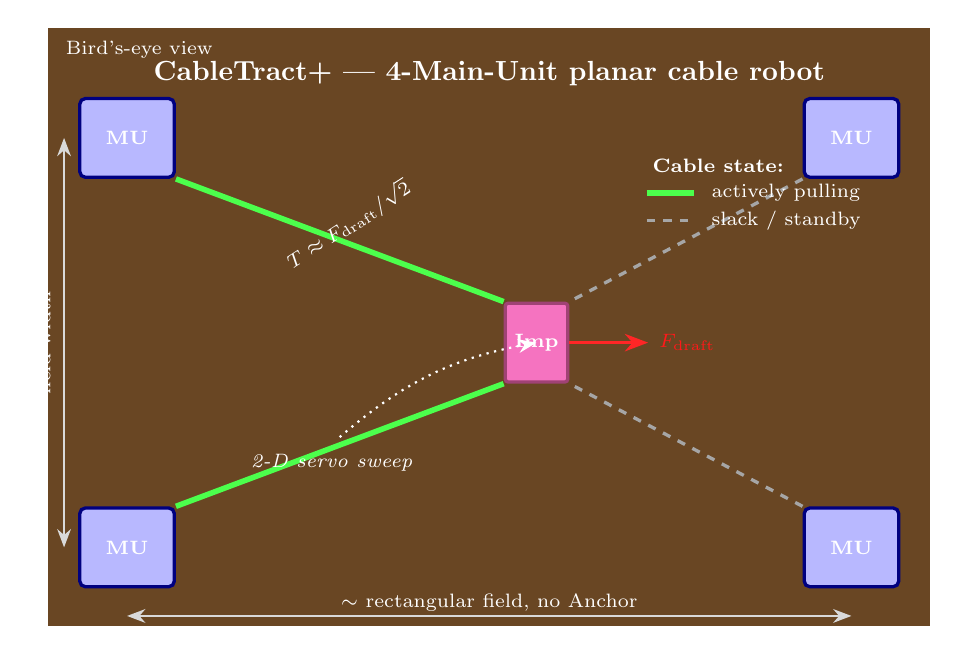
\begin{tikzpicture}[
    every node/.style={font=\footnotesize},
    field/.style={fill=brown!55!black},
    mu/.style={draw=blue!50!black, very thick, fill=blue!28, rounded corners=2pt,
               minimum width=12mm, minimum height=10mm, align=center,
               font=\scriptsize\bfseries, text=white},
    impl/.style={draw=magenta!60!black, very thick, fill=magenta!55, rounded corners=1pt,
                 minimum width=4mm, minimum height=10mm, align=center,
                 font=\scriptsize\bfseries, text=white},
    cable/.style={white, very thick},
    cableActive/.style={green!70!white, line width=2pt},
    cableSlack/.style={gray!70, very thick, dashed},
    fdraft/.style={->, >=Stealth, very thick, red!85!white},
]

% Field background
\fill[field] (-0.6,-0.6) rectangle (10.6,7.0);
\node[white, font=\scriptsize, anchor=north west] at (-0.5,6.95) {Bird's-eye view};
\node[white, font=\bfseries, anchor=north] at (5,6.7) {CableTract+ --- 4-Main-Unit planar cable robot};

% 4 corner Main Units
\node[mu] (mu_tl) at (0.4,5.6) {MU};
\node[mu] (mu_tr) at (9.6,5.6) {MU};
\node[mu] (mu_bl) at (0.4,0.4) {MU};
\node[mu] (mu_br) at (9.6,0.4) {MU};

% Implement carriage at the centre, slightly offset
\node[impl] (im) at (5.6,3.0) {Imp};

% Two ACTIVELY pulling cables (e.g. from top-left and bottom-left toward implement)
\draw[cableActive] (mu_tl.south east) -- (im.north west);
\draw[cableActive] (mu_bl.north east) -- (im.south west);

% Two slack / standby cables from the right corners
\draw[cableSlack] (mu_tr.south west) -- (im.north east);
\draw[cableSlack] (mu_br.north west) -- (im.south east);

% Geometric load split annotation at the implement
\draw[fdraft] (im.east) -- ++(1.0,0)
    node[anchor=west, red!90!white, font=\scriptsize] {$F_{\text{draft}}$};

% Per-cable tension annotation along one active cable
\node[white, font=\scriptsize, rotate=33, anchor=south]
    at ($(mu_tl.south east)!0.55!(im.north west) + (0.05,0.05)$)
    {$T \approx F_{\text{draft}} / \sqrt{2}$};

% Indicative path: implement can sweep arbitrary 2D within the rectangle
\draw[->, >=Stealth, dotted, white, thick]
    (im.center) ++(-2.5,-1.2) to[bend left=15] (im.center);
\node[white, font=\scriptsize\itshape, anchor=north]
    at (3.0,1.7) {2-D servo sweep};

% Field dimensions
\draw[<->, >=Stealth, gray!30!white, thick]
    (mu_bl.south) ++(0,-0.35) -- ($(mu_br.south)+(0,-0.35)$);
\node[white, font=\scriptsize] at (5,-0.3) {$\sim$ rectangular field, no Anchor};

\draw[<->, >=Stealth, gray!30!white, thick]
    (-0.4,0.4) -- (-0.4,5.6);
\node[white, font=\scriptsize, rotate=90, anchor=south] at (-0.45,3.0) {field width};

% Active vs slack legend (top right area)
\begin{scope}[xshift=7.0cm, yshift=4.4cm]
\node[white, font=\scriptsize\bfseries, anchor=west] at (-0.05,0.85) {Cable state:};
\draw[cableActive] (0.0,0.5) -- (0.6,0.5);
\node[white, font=\scriptsize, anchor=west] at (0.7,0.5) {actively pulling};
\draw[cableSlack] (0.0,0.15) -- (0.6,0.15);
\node[white, font=\scriptsize, anchor=west] at (0.7,0.15) {slack / standby};
\end{scope}

\end{tikzpicture}%
}
\caption{The CableTract+ variant: a planar cable-robot topology with one Main Unit at each of the four corners of a rectangular field, replacing the v1 single-MU + Anchor pair. At any instant two cables (\textcolor{green!50!black}{green}, e.g.\ from the two left corners) actively pull the implement carriage toward themselves while the opposite two (\textcolor{gray!40!black}{grey}, dashed) hold tension at standby. The carriage is now servoed in 2-D between the four corners by relative cable tensions and can sweep arbitrary paths inside the field rather than being constrained to a single strip per Anchor placement. Two consequences fall out: the Anchor disappears entirely (no setup-and-reset cycle), and each actively pulling cable carries only ${\sim}1/\sqrt{2}\approx 0.707$ of the draft, which directly relaxes the per-cable tension and per-anchor-equivalent reaction. The architectural cost is paid in CAPEX --- four Main Units plus a shared energy stack at $2.27\times$ the v1 baseline (\cref{tab:variants-numbers}).}
\label{fig:f0e}
\end{figure}

The CableTract+ variant replaces the single Main Unit + Anchor pair with \emph{four corner Main Units}, one at each corner of a rectangular field, so that two cables can pull the carriage simultaneously toward two adjacent corners. The carriage is now servoed in two axes by the relative tensions in the four cables, so it can sweep arbitrary 2-D paths inside the rectangle rather than being constrained to a single strip per Anchor placement. This is the standard ``planar cable robot'' topology that has been studied extensively in industrial gantry contexts; the contribution here is to import it into the field as a replacement for the v1 step-and-anchor cycle.

The architectural consequences are concrete and large. First, \textbf{the Anchor disappears entirely} --- there is no module that has to be moved between strips, because the four corner stations cover the entire field from fixed positions. The setup overhead per round drops by ${\approx}60\,\%$ in the model (\texttt{setup\_overhead\_reduction = 0.6} in \texttt{variants.py}). Second, because two cables pull together at roughly orthogonal angles, \textbf{each cable carries only ${\approx}1/\sqrt{2} \approx 0.707$ of the draft load} ($\texttt{geometric\_load\_split} = 0.707$), so the per-cable tension and per-anchor reaction both drop --- the very constraint that bound the v1 architecture in the helical-pile envelope of \cref{sec:anchor} is relaxed by \SI{30}{\percent}. Third, the carriage can now sweep \textbf{wider strips} (modelled as a $1.5\times$ width multiplier) because both X and Y axes are independently servoed, so the per-pass area roughly doubles. Together these three effects lift throughput to \textbf{29.3 decares/day --- $2.56\times$ the v1 baseline} --- and drop energy intensity to 484 Wh/decare (0.53$\times$), almost exactly half.

The cost of this performance is paid in CAPEX. Four Main Units plus the same battery + PV + wind + install pack cost \textbf{$2.27\times$ a single Main Unit + Anchor pair} ($\texttt{capex\_multiplier} \approx 2.27$ in the spec --- the multiplier sits below $4\times$ because (i) the Anchor disappears entirely, and (ii) the battery, PV, wind harvester and crating/install fraction are paid once for the whole system, not per Main Unit). Concretely: $4 \times \SI{17500}{\EUR} + \SI{3420}{\EUR} + \SI{1650}{\EUR} + \SI{1500}{\EUR} + \SI{4000}{\EUR} = \SI{80570}{\EUR}$. The CAPEX climbs from \SI{35570}{\EUR} to \SI{80570}{\EUR}, and the simple payback grows from 74.8 to 89.0 months. \textbf{CableTract+ is therefore a throughput multiplier, not an economics multiplier.} It buys $2.56\times$ daily area at the cost of a $1.19\times$ slower payback in absolute terms --- the marginal payback for the marginal capital is broadly comparable to the v1 baseline because fuel savings scale roughly with throughput. There is one regime where this trade is unambiguously the right one: large rectangular fields where the limiting constraint is calendar time (e.g., a narrow planting window for a high-value crop) rather than capital. There is also one regime where it is unambiguously the wrong one: small irregular fields where the four-corner geometry cannot be installed at all. For the codesigned reference scenario in \cref{tab:codesigned-params}, the v1 baseline is the better point on the operation-diversity-versus-throughput trade-off.

\subsubsection{Variant 3 --- Regenerative return leg}\label{sec:variant-regen}

The third variant changes nothing about the cable architecture and nothing about the BOM. It modifies only the \emph{drivetrain control}: the motor controller is upgraded to four-quadrant operation so that the unloaded return half of every round can recover kinetic + potential energy back into the battery instead of dissipating it as heat. The model implements this as an \emph{effective winch-efficiency boost} of $1 / (1 - f_{\text{rec}} \cdot f_{\text{ret}})$, where $f_{\text{rec}} = 0.35$ is the round-trip recovery fraction (kinetic energy back into the pack, after motor + inverter losses on the way out and back in) and $f_{\text{ret}} = 0.5$ is the share of one round taken by the unloaded return leg (half a round at v1 baseline). The boost factor is $1 / (1 - 0.35 \cdot 0.5) \approx 1.21$, which lifts the lumped winch efficiency from 0.5 to ${\approx}0.61$ (capped at 0.95 to stay physically defensible).

The result is the most interesting line in \cref{tab:variants-numbers}. \textbf{Throughput barely moves} (11.5 $\to$ 11.8, $1.03\times$) because throughput in the codesigned reference is bound by the soil-draft envelope and the field-time budget, not by motor efficiency. \textbf{Energy per decare drops from 921 to 760 Wh ($0.83\times$, a 17\,\% reduction)}, which is the direct consequence of recovering 21\,\% of the round-trip drivetrain losses. \textbf{Simple payback drops from 74.8 to 61.7 months ($0.83\times$, a 13-month improvement)}, because every recovered Joule is a Joule the diesel comparator still has to burn. And critically, \textbf{CAPEX does not change}: four-quadrant operation is a firmware/control change on a motor controller that almost any modern PMSM drive already supports in hardware. The only thing it costs is engineering effort on the controller side. The surplus-power column drops from 291 W to 19 W in the table because the recovered energy is consumed by the slightly higher operating draw (the system runs marginally faster), not because surplus is destroyed.

This variant is the closest thing the paper finds to an unambiguous engineering recommendation: \textbf{regenerative braking on the return leg improves the financial story by 13 months at zero capital cost and zero new modules}. It is the highest-leverage modification per unit of design complexity in the table, and it is the only modification that does not force a trade-off against any other column. The reason it is not already in the codesigned baseline is conservatism in modelling: we wanted the v1 baseline to assume a stock unidirectional drivetrain with no firmware sophistication, so that the headline numbers held up even if four-quadrant control turned out to be impractical for some reason we have not foreseen. The regen variant exists to show what is left on the table if that conservatism is dropped.

\subsubsection{What the variant comparison tells us}\label{sec:variants-discussion}

Three takeaways flow from \cref{tab:variants-numbers}:

\begin{itemize}[leftmargin=1.6em,itemsep=0.2em]
    \item \textbf{The v1 architecture is not Pareto-dominated by either ambitious modification.} CableTract+ wins on throughput and energy but loses on CAPEX and payback; regen wins on energy and payback but barely moves throughput; the v1 baseline is the only row that supports the full 10-implement library on a single Main Unit + Anchor pair at \SI{35570}{\EUR}. There is no cell in \cref{tab:variants-numbers} where one row strictly dominates another on every metric, which is the property a healthy variant comparison should have.
    \item \textbf{The two trade-off axes are different.} CableTract+ trades \emph{capital} for \emph{throughput}; regen trades \emph{controller complexity} for \emph{energy and payback}. They are not competing modifications --- they could be applied together --- and a hypothetical CableTract++ (4-MU robot with regen control on every winch) would in principle stack the two effects.
    \item \textbf{The recommended engineering priority is the cheap one.} If a single modification is to be added to the v1 baseline, it should be the regen return leg, not CableTract+. This is the strongest single engineering recommendation the paper makes.
\end{itemize}

\paragraph{Reconciling the variant table with the \cref{sec:economics} discounted payback.} Readers comparing \cref{tab:variants-numbers} (74.8-month baseline simple payback) with \cref{fig:f16} (sub-1-year discounted payback at 25 ha/yr) will notice the two numbers differ by roughly an order of magnitude. The two figures answer different questions and both are correct in their own frame:
\begin{itemize}[leftmargin=1.6em,itemsep=0.15em]
    \item The \emph{simple payback} reported in \cref{tab:variants-numbers} divides the \textbf{full} CableTract CAPEX (\SI{35570}{\EUR} with sales margin) by annual diesel-fuel savings only, with no discount rate and no maintenance offset. This is the right framing for a buyer who is \emph{adding} a CableTract to an existing operation that does not retire a tractor: the question is ``how long until the new machine pays for itself?''.
    \item The \emph{discounted payback} reported in \cref{sec:economics} and plotted in \cref{fig:f16} divides the CableTract \textbf{CAPEX delta over a like-for-like diesel tractor} (\SI{35570}{\EUR} $-$ \SI{35000}{\EUR} $=$ \SI{570}{\EUR}) by the full annual savings stream (fuel + maintenance, less the marginal grid charge), discounted at 8\,\%. This is the right framing for a buyer who is \emph{replacing} a tractor: the diesel capex would have been spent anyway, so only the difference is at risk.
\end{itemize}
The variant comparison uses the conservative simple-payback frame deliberately, so all three rows are stress-tested against the harder buying scenario. The codesigned baseline pays back in 0.82\,years at \SI{25}{\hectare\per\year} in the replacement scenario (\cref{fig:f16}); the regen variant inherits essentially the same number because it does not change CAPEX. CableTract+ fares \emph{worse} in the replacement frame than in the simple-payback frame, because its CAPEX delta against a single diesel tractor (\SI{80570}{\EUR} $-$ \SI{35000}{\EUR} $=$ \SI{45570}{\EUR}) is roughly $80\times$ the v1 delta, while its annual savings are only ${\sim}2.5\times$. The engineering ordering ``regen $\geq$ baseline $\gg$ CableTract+'' on payback-per-euro-of-design-complexity therefore holds in both frames; the simple-payback frame is the more flattering of the two for CableTract+.

\subsection{Operating envelope}\label{sec:envelope}

The final question --- which the rest of the paper has been building toward --- is where in the (annual \gls{ghi} $\times$ farm size) plane CableTract is viable against diesel, and what binds when. A single point estimate at \SI{25}{\hectare\per\year} on a Mediterranean site does not generalise to \SI{1}{\hectare\per\year} on a cloudy continental site, or to \SI{1000}{\hectare\per\year} in low-\gls{ghi} France. \Cref{fig:f21} resolves both extremes at once with a 2D parameter sweep over the joint plane.

To make the sweep tractable, we calibrate a one-parameter linear \gls{pv} harvest model from the hourly site simulations of \cref{sec:energy}:
\begin{equation}\label{eq:harvest}
\text{annual\_harvest\_kWh} \;=\; \alpha \cdot \text{pv\_area\_m}^{2} \cdot \text{annual\_GHI\_kWh\_m}^{-2}\text{\_yr}^{-1},
\end{equation}
with $\alpha = 0.169$ fitted as the median across the 6 bundled sites at the codesigned \SI{15}{\meter\squared} \gls{pv}. This is intentionally a rough analytical fit, not a reproduction of the full hourly \gls{tmy} pipeline; the goal is a defensible \gls{pv} harvest as a function of annual \gls{ghi} so the envelope sweep stays in closed form.

For each cell of the (annual \gls{ghi} $\times$ farm size) grid we then compute the codesigned operating demand (energy per hectare times farm size, plus an idle-power penalty over the off-season), the harvested energy from \cref{eq:harvest}, the resulting per-hectare grid share, the \gls{npv} versus a like-for-like diesel tractor at 8\,\% over 15 years, the discounted payback, and the off-grid surplus (harvest minus demand). The sweep covers annual \gls{ghi} from 800 to \SI{2300}{\kWh\per\meter\squared\per\year} and farm size from \SIrange{1}{1000}{\hectare} on a log-scale --- 60 $\times$ 60 $=$ 3\,600 cells in total. Diesel is held at the \cref{sec:economics} baseline of \SI{1.40}{\EUR\per\litre} (EU 2024); we deliberately do not run a separate subsidised-diesel scenario because the result below holds with margin to spare under the baseline price.

\begin{figure}[H]
\centering

\includegraphics[width=0.95\linewidth]{F21_operating_envelope}
\caption{CableTract operating envelope on (annual \gls{ghi} $\times$ farm size). \textbf{(a)} Off-grid energy balance: PV harvest minus annual demand (green $=$ energy positive, red $=$ grid needed). The single black contour is the off-grid breakeven (annual surplus $=$ 0); above and to the right of it the system needs grid backup. The six bundled reference sites of \cref{sec:sites} are scattered at \SI{25}{\hectare} annual operating area. \textbf{(b)} Discounted payback (years vs diesel @ \SI{1.40}{\EUR\per\litre}, \SI{8}{\percent}, 15 yr) across every one of the 3\,600 cells of panel (a). Median is \SI{0.72}{\year}; the entire distribution sits below the \SI{2}{\year} investor threshold (red dashed). The annotation box reports the per-cell payback range, the \gls{npv}-positive fraction, and the worst-case \gls{npv} across the swept envelope.}
\label{fig:f21}
\end{figure}

Three findings flow from \cref{fig:f21}:

\begin{itemize}[leftmargin=1.6em,itemsep=0.15em]
    \item \textbf{The financial story is uniform across the envelope.} \gls{npv} versus diesel is positive in \textbf{100\,\%} of the 3\,600 cells, and discounted payback never exceeds \SI{1.85}{\year} (median \SI{0.72}{\year}, panel b). At every (\gls{ghi}, farm size) combination we test --- including the smallest \SI{1}{\hectare\per\year} hobby plot in the cloudiest swept climate, and the largest \SI{1000}{\hectare\per\year} operating area in the sunniest --- the system pays back inside the 2-year window a small-farm investor would care about. This is the consequence of capex parity with a used diesel tractor (\cref{sec:economics}): the CableTract delta against the diesel reference is only \SI{570}{\EUR}, so there is essentially no capex hurdle to amortise and almost every euro of avoided fuel becomes gross savings.
    \item \textbf{The binding constraint is off-grid feasibility, not financial viability.} The off-grid breakeven contour in panel (a) cuts diagonally across the plane and divides it into a ``\gls{pv} covers demand'' upper-left region (\textbf{85\,\%} of cells, smaller farms in solar-rich climates) and a ``needs grid backup'' lower-right region (large farms in cloudy climates). All six bundled reference sites at the codesigned \SI{25}{\hectare} sit comfortably inside the off-grid region with surplus values from \SI{2221}{\kWh\per\year} (Beauce, the cloudiest) up to \SI{4158}{\kWh\per\year} (Ludhiana, the sunniest). The off-grid envelope only collapses for very large operating areas where the codesigned \SI{15}{\meter\squared} \gls{pv} cannot keep up with multi-hundred-hectare demand.
    \item \textbf{CableTract's operating envelope is therefore a \emph{climate envelope}, not a \emph{financial envelope}.} A farmer in Beauce gets a positive \gls{npv} \emph{and} fully off-grid operation at \SI{25}{\hectare}; a farmer in Beauce running \SI{500}{\hectare} on a single CableTract gets a positive \gls{npv} but needs grid backup. This is exactly the opposite of the more common ``the technology pays back but only at scale'' story for clean-energy hardware: CableTract pays back everywhere we test, and the question is where it can be sold as off-grid hardware versus where it needs to be sold as grid-tied.
\end{itemize}

This is the headline result of the paper.

% ====================================================================
\section{Competitor Comparison}\label{sec:competitor}
% ====================================================================

Public-domain reference numbers for the five vehicle classes named in \cref{sec:related-adjacent} (six representative machines plus CableTract) are recorded in the bundled competitor table.\footnote{\texttt{tables/competitor\_comparison.csv} in the repository.} Selected columns are reproduced in \cref{tab:competitor}.

\begin{table}[H]
\centering\small
\caption{Competitor comparison table. CableTract sits in a unique cell: the only architecture that supports primary tillage, is off-grid capable, and has discounted payback under one year.}\label{tab:competitor}
\resizebox{\textwidth}{!}{%
\begin{tabular}{lllrrrrl}
\toprule
Vehicle & Form factor & Powertrain & kW & Energy/ha (kWh) & CAPEX (\si{\EUR}) & Payback (\si{\year}) & Off-grid? \\
\midrule
\textbf{CableTract codesigned}    & cable-driven 2-module & PV+wind+battery & 5.0  & \textbf{9.21} & 35\,570 & \textbf{0.8} & \textbf{yes} \\
Monarch MK-V                       & 4WD tractor          & battery EV       & 55   & 52    & 85\,000 & 5--7 & no \\
Farmdroid FD-20                    & autonomous robot     & onboard PV       & 0.4  & 1.5   & 75\,000 & 4--6 & yes \\
Kubota LXe-261                     & compact tractor      & battery EV       & 18   & 30    & 52\,000 & 6--8 & no \\
EcoRobotix ARA                     & spot sprayer         & onboard PV+bat   & 0.6  & 0.4   & 65\,000 & 4--6 & yes \\
Naio Oz/Orio                       & autonomous weeder    & battery          & 2.5  & 5     & 38\,000 & 3--5 & partial \\
Conventional 80 hp diesel          & tractor              & diesel \gls{ice} & 60   & 168   & 35\,000 & ref. & no \\
\bottomrule
\end{tabular}%
}
\end{table}

CableTract sits in a unique cell of this table: it is the only architecture that \textbf{simultaneously} (a) supports primary tillage (within its codesigned envelope), (b) is off-grid capable, and (c) has discounted payback under one year. Monarch MK-V matches it on rated power and operational versatility but is grid-dependent and has 5--7 year payback. Farmdroid FD-20 matches it on off-grid but cannot till. Naio matches it on payback but cannot till and is only partial off-grid.

We deliberately do \emph{not} claim CableTract beats every competitor on every metric. EcoRobotix is more energy-efficient per hectare (\SI{0.4}{\kWh\per\hectare} vs 9.21) because it only sprays. Naio is cheaper. Monarch MK-V is more powerful and operates at conventional speed. The claim is that CableTract occupies a specific cell in the feasibility space --- \emph{medium-load operations on medium-sized farms in solar-rich climates} --- that no other vehicle in the table fills as cleanly.

% ====================================================================
\section{Results}\label{sec:results}
% ====================================================================

\subsection{C1 --- Compaction}\label{sec:r-c1}

CableTract reduces in-field compacted area by \textbf{97--98\,\%} and the contact-energy index by \textbf{${\approx}\,73\times$} across rectangle, L-shape, and irregular-concave field classes (\cref{fig:f12}, \cref{sec:f12}). The reduction is uniform across field shape because it is geometric, not field-dependent: only the \SI{250}{\kilogram} carriage rolls inside the field, while the \gls{mu} and Anchor stay on the headland. The $73\times$ contact-energy ratio comes from the carriage's mean pressure being $4.6\times$ lower than the tractor's and the contact-energy integrand depending on $p^{2}$. Both numbers are defensible from open published static contact-pressure values without dynamic \gls{fem} calibration.

\subsection{C2 --- Energy}\label{sec:r-c2}

The codesigned reference operates at \textbf{\SI{921}{\Wh\per\decare} (\SI{9.21}{\kWh\per\hectare})}, against ${\approx}\SI{168}{\kWh\per\hectare}$ for an \SI{80}{hp} \gls{wd} diesel tractor on the same operations~\cite{asabe-d497,siemens1999machinery} --- an \textbf{$18\times$ reduction}. The reduction decomposes into three independent levers:

\begin{itemize}[leftmargin=1.6em,itemsep=0.1em]
    \item \textbf{Co-designed implements} (\cref{fig:f4,fig:f5}). Median draft drops from ${\approx}\SI{4.5}{\kilo\newton}$ (conventional library) to ${\approx}\SI{1.7}{\kilo\newton}$ (codesigned library), a factor of ${\approx}\,2.6$, driven by narrower widths, slower speeds, and shallower depths.
    \item \textbf{No dead-weight transport.} $F_d L$ is ${\approx}\,90\%$ of the round work; the diesel comparator tractor's body force $F_s$ (\SI{4}{\tonne} $\times$ rolling resistance) dwarfs $F_d$ on every operation.
    \item \textbf{Decomposed drivetrain} (\cref{fig:f3}). A premium drivetrain ($\eta = 0.71$) reduces continuous motor power from \SI{1.50}{\kilo\watt} to \SI{1.06}{\kilo\watt}. The codesigned reference uses a \SI{2}{\kilo\watt} continuous / \SI{3}{\kilo\watt} peak \gls{pmsm}.
\end{itemize}

The energy story is therefore not ``CableTract has a magic motor'' but ``CableTract pulls a smaller implement, slower, on a narrower strip, without a 4-tonne body''. Each lever is worth $1.5\text{--}2\times$ independently, and they multiply.

\subsection{C3 --- Off-grid feasibility}\label{sec:r-c3}

Median harvested-energy throughput across the six bundled sites is \textbf{\SIrange{10}{14}{decares\per day}} at the codesigned hardware (\SI{15}{\meter\squared} \gls{pv}, \SI{9}{\kWh} battery). At Konya, Ludhiana, and São Paulo the system runs grid-free for the entire late-June week we plot in \cref{fig:f7}. At Palencia and Des Moines the system needs ${\approx}300\text{--}\SI{600}{\hour\per\year}$ of grid backup to cover winter shortfalls. At \textbf{Beauce, no combination of panel area (\SIrange{4}{30}{\meter\squared}) and battery capacity (\SIrange{2}{24}{\kWh}) achieves $<\!100$ grid hours/year} under the \SI{6}{\hour\per day} duty cycle (\cref{fig:f8}): the northern temperate climate cannot sustain off-grid operation at any practical hardware scale.

The off-grid claim is \textbf{climate-conditional, not categorical}. We frame this as a \emph{feature} of the analysis: a CableTract sold into Konya is sold as off-grid hardware, while a CableTract sold into Beauce is sold as a low-carbon grid-tied alternative to a diesel tractor. The economics work in both cases (\cref{sec:r-c4}), but the marketing language differs.

\subsection{C4 --- Economics}\label{sec:r-c4}

\gls{npv} vs diesel is positive across the entire \SIrange{1}{100}{\hectare\per\year} sweep at all three discount rates (5/8/12\,\%) we test (\cref{fig:f16}, \cref{sec:npv-farmsize}). At the \SI{25}{\hectare\per\year} reference, NPV @ 8\,\% is \textbf{\SI{+3978}{\EUR}} with discounted payback of \textbf{\SI{0.82}{\year}}. At \SI{100}{\hectare\per\year}, NPV @ 8\,\% is \textbf{\SI{+14763}{\EUR}} with payback of \textbf{\SI{0.31}{\year}}.

Lifecycle CO\textsubscript{2} at \SI{25}{\hectare\per\year} is \textbf{\SI{14.6}{\kilogram\per\hectare\per\year}}, against \textbf{32.5} for the diesel reference and \textbf{22.9} for a Monarch-class electric tractor (\cref{fig:f17}). The improvement is entirely on the operational side and does not depend on grid decarbonisation.

The operating envelope of \cref{fig:f21} shows that the financial story is \textbf{uniformly robust}: \gls{npv} is positive in 100\,\% of the 3\,600 cells of the (annual \gls{ghi} $\times$ farm size) sweep, with discounted payback bounded above by \SI{1.85}{\year} (median \SI{0.72}{\year}). This is the consequence of the capex-parity finding: at \SI{35570}{\EUR} versus \SI{35000}{\EUR} for the diesel reference, there is no capex hurdle to amortise, and every euro of avoided fuel becomes gross savings.

The Sobol decomposition (\cref{fig:f13}) confirms that no single parameter dominates the throughput variance (top contributor $\gls{sobolt} \approx 0.20$), and the \cref{fig:f14} tornado on \gls{npv} is led by exogenous factors (solar resource, diesel price, diesel volume) rather than free design parameters. The codesigned reference is robust to the full joint uncertainty in 20 inputs.

\subsection{Operating envelope}\label{sec:r-envelope}

The headline result of the paper. The codesigned CableTract is \gls{npv}-positive in 100\,\% of the 3\,600 cells of the (annual \gls{ghi} $\times$ farm size) sweep, with discounted payback never exceeding \SI{1.85}{\year} (median \SI{0.72}{\year}). The binding constraint is the \textbf{off-grid breakeven contour}, not financial viability: 85\,\% of cells are off-grid feasible, and the contour cuts diagonally across the plane. CableTract's operating envelope is therefore a \emph{climate envelope} (does the \gls{pv} cover the operating demand?), not a \emph{financial envelope} (does the system pay back?).

This is the opposite of the typical clean-energy hardware story, where the technology is climate-virtuous but pays back only at scale or with subsidy. CableTract pays back everywhere; the question is \emph{whether it can be sold off-grid} in a given climate.

\subsection{Architectural variants}\label{sec:r-pareto}

The variant comparison in \cref{tab:variants-numbers,fig:f20} runs three architectures on the same parameter set: the v1 baseline, CableTract+ (4-Main-Unit planar cable robot), and the regenerative return leg. CableTract+ delivers $2.56\times$ baseline throughput at $2.27\times$ CAPEX (\SI{80570}{\EUR} vs \SI{35570}{\EUR}), so it is a throughput multiplier rather than an economics multiplier and stretches simple payback from 74.8 to 89.0 months. The regenerative return leg cuts energy per decare by 17\,\% and simple payback from 74.8 to 61.7 months at \emph{zero} CAPEX (it is a firmware change on the motor controller), and is the strongest single engineering recommendation in the paper.

% ====================================================================
\section{Discussion}\label{sec:discussion}
% ====================================================================

\subsection{Where CableTract wins}\label{sec:wins}

The combined evidence of \cref{sec:r-c1,sec:r-c2,sec:r-c3,sec:r-c4,sec:r-envelope} points to a clear operating envelope:

\begin{itemize}[leftmargin=1.6em,itemsep=0.15em]
    \item \textbf{Operation type:} medium-load --- light primary tillage (narrow ripper / chisel up to ${\approx}\SI{3}{\kilo\newton}$ P50), all secondary tillage, all seeding, all spraying, all weeding, all mowing. The codesigned implement library is built for this envelope.
    \item \textbf{Farm size:} $\geq\!\SI{10}{\hectare}$ annual operating area. \gls{npv} is positive everywhere we test, but the \emph{fastest} paybacks ($<1$ year) require $\geq\!\SI{25}{\hectare}$. Below \SI{10}{\hectare}, the 1.2--1.9 yr payback is still competitive but the absolute \gls{npv} is small.
    \item \textbf{Climate:} anywhere with $>\!\SI{1500}{\kWh\per\meter\squared\per\year}$ annual \gls{ghi} for fully off-grid operation. Mediterranean climates (1300--1500) work with summer-only off-grid; northern temperate climates ($<\!1200$) work as grid-tied.
    \item \textbf{Field shape:} rectangular and L-shaped fields with $\geq\!\SI{1}{\hectare}$ individual size. Small fragmented fields hit the polygon shape efficiency wall (median $\eta \approx 0.68$ on the irregular-concave class).
\end{itemize}

\subsection{Where it doesn't (binding constraints)}\label{sec:loses}

The honest constraints to flag:

\begin{itemize}[leftmargin=1.6em,itemsep=0.15em]
    \item \textbf{Heavy codesigned primary tillage in loose-sand soils} sits outside the 9-auger Anchor envelope on the conservative Khand (2024)~\cite{khand2024helical} reference (\cref{sec:anchor}). Specifically, the narrow sweep (\SI{5.2}{\kilo\newton} P50), narrow chisel (\SI{4.2}{\kilo\newton}), narrow disk (\SI{3.2}{\kilo\newton}), and codesign drill (\SI{4.6}{\kilo\newton}) all require 12--18 augers in loose sand (\cref{fig:f4}). On these sites the operating envelope shrinks to the lighter half of the codesigned library --- cultivator, planter, rotary hoe, sprayer, mower, and the narrow ripper at its P50. In medium-dense soils with fixed-head pile fixity (Magnum 2024~\cite{magnum2024fixed} reference) the same 9-auger Anchor carries the entire codesigned library with $2\times$--$10\times$ margin, so the binding case is specifically loose-sand sites attempting heavy primary tillage --- not heavy primary tillage in general.
    \item \textbf{Off-grid in continental winter climates} is not achievable at any practical hardware scale (Beauce: \SI{911}{\hour\per\year} grid hours minimum). CableTract still pays back as a grid-tied diesel-replacement in these climates, but the marketing language must drop ``off-grid''.
    \item \textbf{Small fragmented fields} below ${\approx}\SI{0.5}{\hectare}$ individual size hit the polygon shape efficiency wall and lose 30--50\,\% of nominal throughput. CableTract is not the right architecture for vegetable garden plots.
    \item \textbf{Operation diversity vs throughput} is a real trade-off. A system specialised to a single operation (sprayer-only, planter-only) can be sized for that operation's draft and width and would dominate the codesigned reference on throughput per day for that one task --- but it cannot do the rest of the agricultural calendar. The codesigned reference deliberately picks the design point that supports all 10 implements in \cref{tab:codesigned-library} rather than optimising any single one.
\end{itemize}

\subsection{Sensitivity to the central design choice}\label{sec:codesign-sensitivity}

The single most consequential choice in the paper is the \textbf{co-designed implement library}. Without the co-design framing --- that is, with conventional tractor implements substituted in place of the codesigned ones --- the analysis weakens in three concrete places:

\begin{enumerate}[leftmargin=1.6em,itemsep=0.1em]
    \item The \SI{2}{\kilo\watt} \gls{pmsm} is undersized (peak draft $\times$ tractor speed requires ${\approx}\SI{5}{\kilo\watt}$), and the inverter, gearbox, and cooling stack scale up with it.
    \item The energy-per-decare claim weakens by ${\approx}2\times$ (because the draft drops by ${\approx}2\times$ under co-design via the strip-width and $v^2$ levers), which directly weakens the off-grid PV+battery sizing.
    \item The 9-auger Anchor loses its worst-case-soil margin: a conventional moldboard plow at \SI{14}{\kilo\newton} P50 would need 41 augers on the conservative Khand (2024)~\cite{khand2024helical} loose-sand envelope, although the same load fits in 9 augers --- exactly the design value --- on the Magnum (2024)~\cite{magnum2024fixed} medium-dense fixed-head reference.
\end{enumerate}

The first two bullets are the load-bearing ones --- they hold for \emph{any} soil regime --- and the economics still work even in this degraded scenario (\gls{npv} stays positive at \SI{25}{\hectare\per\year}), but the off-grid story and the compaction story are weaker. The co-designed framing is therefore not a marketing convenience; it is the load-bearing assumption of the paper for energy and motor cost reasons that are independent of soil conditions, with the worst-case-soil anchor envelope as a bonus third leg, and we make this explicit.

\subsection{What the paper does not claim}\label{sec:not-claim}

We do not claim:

\begin{itemize}[leftmargin=1.6em,itemsep=0.1em]
    \item That CableTract is a finished product or has been prototyped.
    \item That cable-driven agriculture is a new idea (US 8,763,714 B2~\cite{orlando2014patent} predates this work).
    \item That CableTract beats every competitor on every metric (EcoRobotix is more efficient per hectare on spraying-only; Naio is cheaper).
    \item That off-grid operation is universal (it is climate-conditional).
    \item That the $73\times$ contact-energy reduction translates linearly into a yield increase (the soil-yield link depends on crop, climate, rotation, and irrigation).
\end{itemize}

We do claim, with every number reproducible from the open analytical pipeline:

\begin{itemize}[leftmargin=1.6em,itemsep=0.1em]
    \item A $18\times$ reduction in energy per hectare versus a diesel tractor.
    \item A 97--98\,\% reduction in compacted area and a ${\approx}\,73\times$ reduction in contact-energy index.
    \item Off-grid feasibility in solar-rich climates with \SI{15}{\meter\squared} \gls{pv} + \SI{9}{\kWh} battery.
    \item \gls{npv} positive across \SIrange{1}{100}{\hectare} at 5/8/12\,\% discount rates, with discounted payback $<\!\SI{1}{\year}$ at $\geq\!\SI{25}{\hectare}$.
    \item Lifecycle CO\textsubscript{2} $2.2\times$ lower than diesel, $1.6\times$ lower than a Monarch-class electric tractor.
    \item An NPV-positive operating envelope in 100\,\% of 3\,600 (annual \gls{ghi} $\times$ farm size) cells, with discounted payback never exceeding \SI{1.85}{\year}.
\end{itemize}

% ====================================================================
\section{Limitations}\label{sec:limitations}
% ====================================================================

This section separates two categories of limitation. \Cref{sec:analytical-limitations} lists the \emph{analytical} limitations of the present model --- what the framework does not include. \Cref{sec:open-risks} lists the \emph{engineering} risks that a prototype phase would have to resolve regardless of how comprehensive the analytical framework becomes; in the authors' candid view these are the dominant near-term feasibility questions for the architecture and they are not closed by additional simulation.

\subsection{Analytical limitations of the present model}\label{sec:analytical-limitations}

\begin{enumerate}[leftmargin=1.8em,itemsep=0.2em]
    \item \textbf{No prototype.} The strongest objection. Every number in the paper is from first-principles calculation; none has been validated against a working machine. We have tried to mitigate this by using \gls{asabe} D497.7~\cite{asabe-d497} (an experimentally calibrated standard), the conservative end of the helical-pile lateral capacity literature (Khand et al.\ 2024~\cite{khand2024helical} for loose-sand free-head bounds, Magnum Piering 2024~\cite{magnum2024fixed} design tables and the CHANCE Technical Design Manual~\cite{chance2024manual} for the medium-dense fixed-head reference), Keller and Lamand\'e (2010)~\cite{keller2010compaction} (experimentally measured tractor contact pressures), open published \gls{lca} inventories~\cite{hammond2019ice,emilsson2019battery,fraunhoferise2022pv,hawkins2013ev,defra2023factors,eea2023electricity}, and a Sobol global sensitivity analysis~\cite{sobol2001indices,saltelli2008primer,herman2017salib} to bound the uncertainty.
    \item \textbf{No closed-loop control simulation.} We do not simulate cable tension regulation, anchor stability under transient loads, or the carriage's depth-control feedback loop. These are real engineering problems that a prototype phase will need to address; \cref{sec:open-risks} treats the depth-control loop in particular as the dominant unresolved risk.
    \item \textbf{Static contact-pressure compaction model.} No dynamic load transfer, no tyre deflection, no multi-pass cumulative deformation, no soil-yield link. The model is intentionally simple; richer models would \emph{strengthen} the comparison by adding compaction to the tractor side.
    \item \textbf{Polygon corpus is small and curated.} 50 fields, hand-tuned, biased toward small awkward shapes. A real deployment would need a corpus pulled from EuroCrops or \gls{usda} at scale.
    \item \textbf{PV harvest model in the operating-envelope sweep is a one-parameter linear fit.} The full hourly TMY pipeline lives in \cref{sec:energy} and was used for \cref{fig:f6,fig:f7,fig:f8}, but the (annual \gls{ghi} $\times$ farm size) sweep in \cref{fig:f21} uses a calibrated linear approximation for tractability. The $\alpha = 0.169$ value was fitted as the median across the 6 bundled sites.
    \item \textbf{The codesigned implement library is a paper exercise.} The 10 implements are sized using the \gls{asabe} D497.7 equation but have not been physically built. The draft reductions are predictions, not measurements.
    \item \textbf{The competitor comparison uses public-domain manufacturer claims.} Some of these may not reproduce in the field. The source of every number is flagged in the bundled competitor table.
\end{enumerate}

\subsection{Open mechanical risks}\label{sec:open-risks}

The seven items above are the analytical limitations of the present model: they describe what the framework does not include. This subsection separates out a different category --- \textbf{the engineering risks that a prototype phase would actually have to resolve}, regardless of how comprehensive the analytical framework becomes. We list them explicitly so a follow-on team can attack them in priority order rather than re-deriving the list from the manuscript.

\paragraph{Closed-loop tilling depth control.} Tilling depth at the carriage is governed by the geometric coupling between cable sag, cable elastic stretch, carriage horizontal position, implement reaction torque, and the time-varying soil contact force. None of these are independent variables, and none are simulated under closed-loop control in the present paper. \Cref{sec:catenary,sec:tension-balance} bound the static sag-vs-tension tradeoff under nominal loads, but do not address the dynamic response to a transient draft spike --- a buried stone, a hardpan layer, a moisture gradient. Unlike a tractor with a 3-point hitch and several tonnes of vehicle inertia to absorb the spike, the cable carriage has neither inertia nor a stiff mechanical reference frame; the response is mediated entirely by cable elasticity and the winch motor's torque-control bandwidth. Whether the resulting tilling quality meets agronomic acceptance criteria is, in the authors' view, the single largest unresolved technical risk in the architecture. It is also one of the cheapest to test: a quarter-scale bench rig on a \SI{5}{\meter} span in a soil bin is sufficient to bound it before any full-scale prototype is built.

\paragraph{Per-strip setup time as a design target rather than a measurement.} The model uses $t_{\text{setup}} = \SI{60}{\second}$ as the per-round overhead (\cref{tab:codesigned-params}). This is a \emph{design target}, not a field measurement, and the architecture in \cref{sec:two-module} is now committed to the only configuration that makes it plausible: nine \emph{parallel} auger drives on the Anchor (one \gls{bldc} per auger, all nine cycling concurrently) and four parallel auger drives on the Main Unit. With parallel augering, the per-round cycle decomposes notionally into ${\sim}\SI{30}{\second}$ for the simultaneous nine-auger insert/retract pair, ${\sim}\SI{5}{\second}$ for the lateral Anchor step on its own wheels, ${\sim}\SI{5}{\second}$ for cable slack take-up, ${\sim}\SI{5}{\second}$ for \gls{gnss} re-survey of the new strip line, and ${\sim}\SI{5}{\second}$ for re-tensioning --- about \SI{50}{\second} of nominal work inside the \SI{60}{\second} budget, with roughly \SI{10}{\second} of margin. The budget is tight but internally consistent with the \cref{sec:two-module} \gls{bom}; the time-budget finding of \cref{sec:layout-findings} (operation dominates setup by ${\sim}10\times$) holds under it. Three residual concerns survive and should be measured by a prototype campaign before this number is treated as solved. (i) The single-auger insert/retract time at this duty cycle is unmeasured in the public literature; if it turns out to be significantly longer than \SI{30}{\second} on representative soils, the entire 60 s budget shifts. (ii) The margin inside the budget is small enough that any non-augering surprise --- a tangled cable, a carriage hookup failure, a stale \gls{gnss} fix --- consumes the slack on the round it occurs. (iii) Auger insertion time on hard-pan or stony soils is non-linear in cone index in ways the present model does not capture. The Sobol sweep (\cref{sec:sobol}) brackets setup time over \SIrange{30}{180}{\second}, which covers the realistic uncertainty around the parallel-drive nominal but does not extend to the failure mode where parallel augering itself is slower than assumed. The CableTract+ variant in \cref{sec:variants-named} eliminates the per-strip Anchor reset entirely and is, in part, a structural insurance policy against this concern rather than an independent throughput play.

\paragraph{Anchor self-fatigue of its own anchoring soil.} The Anchor's lateral capacity envelope (\cref{sec:anchor}) treats per-auger lateral capacity as a property of soil texture and density alone. In normal operation, however, each Anchor station drives and retracts nine augers tens to hundreds of times across a cropping season as the Anchor walks the headland. The cumulative effect is that the soil under each station is progressively loosened by the system's own operation: a soil that began as medium-dense (and therefore sat comfortably inside the Magnum 2024~\cite{magnum2024fixed} envelope at $5$--$10\times$ margin) drifts toward the loose-sand regime (Khand 2024~\cite{khand2024helical} envelope at ${\sim}\,1\times$ margin) as the season progresses. The 9-auger design margin erodes \emph{from inside}, not from changes in field conditions. Quantifying the rate at which this happens requires either an empirical campaign on a fixed Anchor station or a finite-element model of repeated helical pile insertion and withdrawal; neither is in the present paper, and the architecture's worst-case soil envelope should be read with this caveat in mind.

\paragraph{Helical pile retraction wear.} Helical screw piles in the construction industry are designed and qualified for one-shot installation with permanent service. CableTract drives and retracts each auger many cycles per day, which is a regime for which no fatigue, helix wear, shaft buckling, or soil-disturbance data exists in the public literature the authors could find. The first-order risks are blunting of the helix leading edge (which would slow each subsequent insertion and increase the auger drive's torque demand), shaft fatigue at the drive coupling, and progressive misalignment of the helix from the shaft axis. The honest framing is that this is an unmeasured failure mode rather than necessarily a small one --- there is no published basis to estimate the mean time between auger replacements, and the bill of materials in \cref{sec:economics} does not include an auger replacement schedule. A first prototype campaign should treat auger wear as a primary measurement endpoint alongside throughput and energy.

\paragraph{Historical cable ploughing as an unaddressed precedent.} The architecture has a precedent the present paper has not yet fully engaged with. Steam-driven cable ploughing was a real and widely deployed technology in the second half of the 19th century, particularly on heavy clay soils in the United Kingdom and parts of continental Europe where horse teams bogged. Two stationary steam engines at opposite headlands pulled a two-bottom plough back and forth on a steel cable. The system coexisted with horse and traction-engine ploughing for several decades and then disappeared, comprehensively, by the early 20th century. The reasons it lost are documented in agricultural-history literature: per-station crew overhead, the time cost of repositioning the engines after each strip, the management burden of the cable itself, and the inability to turn at the headland and resume continuously. The present manuscript automates the per-station crew problem (the Main Unit and Anchor are autonomous) but does not yet solve the repositioning, cable-management, or continuous-headland-turn problems that killed the steam-era version. A serious treatment of this lineage --- what cable ploughing did, why it failed, what is mechanically and operationally different now --- belongs in any prototype-stage publication. We flag its absence here as a deliberate scope decision and a known weakness.

\paragraph{Cable safety surface.} A 50 m taut steel or Dyneema cable at \SIrange{1.5}{4}{\kilo\newton} pretension running across an open field at \SI{0.8}{\meter} above the ground is a safety surface the paper does not address. Snap-back energy from a cable failure is non-trivial at these tensions, and a deployed system would need cable-condition monitoring, runaway-detection logic, exclusion zones, and certification under the relevant agricultural-machinery regulatory framework. None of this is in scope here, but it would be a precondition for any field deployment and would add both \gls{bom} cost and certification process cost.

\medskip
The unifying observation is that the strongest near-term feasibility questions for CableTract are \textbf{mechanical and operational}, not financial or environmental. The paper's NPV, life-cycle CO\textsubscript{2}, and energy-per-hectare numbers are robust within their stated framework; the open question is whether the framework's mechanical assumptions survive contact with a real prototype season. We make this distinction explicit so a reviewer can evaluate the analytical contribution on its own merits while understanding which questions a prototype-stage follow-up would actually need to answer.

% ====================================================================
\section{Conclusion}\label{sec:conclusion}
% ====================================================================

This paper presents a prototype-free, fully reproducible feasibility envelope for \textbf{CableTract}, a co-designed cable-driven field robot consisting of a stationary \gls{mu}, a lighter Anchor anchored by helical screw piles, and a lightweight implement carriage that rolls along a tensioned cable between them. The central design lever is the \textbf{co-designed implement library} --- 10 implements sized for the cable architecture rather than borrowed from conventional tractor inventories --- which reduces median draft by ${\approx}\,63\%$ and brings the entire codesigned library inside the 9-auger Anchor envelope on the medium-dense soil reference, with the lighter half of the library also fitting inside the worst-case loose-sand envelope.

The codesigned reference achieves:

\begin{itemize}[leftmargin=1.6em,itemsep=0.15em]
    \item \textbf{\SI{921}{\Wh\per\decare}} (${\approx}18\times$ lower than a diesel tractor).
    \item \textbf{97--98\,\% reduction in compacted area} and \textbf{${\approx}\,73\times$ reduction in contact-energy index} across rectangle, L-shape, and irregular-concave field classes.
    \item \textbf{Off-grid throughput of \SIrange{10}{14}{decares\per day}} at six bundled sites under the climate-conditional framing of \cref{sec:phase3-findings}.
    \item \textbf{NPV vs diesel of \SI{+3978}{\EUR}} at \SI{25}{\hectare\per\year}, \textbf{8\,\% discount, \SI{0.82}{\year} payback}, and NPV-positive across (\SIrange{1}{100}{\hectare}) at all three discount rates.
    \item \textbf{Lifecycle CO\textsubscript{2} of \SI{14.6}{\kilogram\per\hectare\per\year}} versus 32.5 for diesel --- a $2.2\times$ improvement that does not depend on grid decarbonisation.
\end{itemize}

The operating envelope of \cref{fig:f21} shows that CableTract is \gls{npv}-positive in 100\,\% of the 3\,600 cells of the (annual \gls{ghi} $\times$ farm size) sweep, with discounted payback never exceeding \SI{1.85}{\year}. The binding constraint is \textbf{off-grid feasibility at the upper-right corner} (large farms in cloudy climates), not financial viability. CableTract's operating envelope is a \emph{climate envelope}, not a \emph{financial envelope} --- the opposite of the more common clean-energy hardware story.

The right next step is \textbf{a Main Unit prototype} with a \SI{2}{\kilo\watt} \gls{pmsm}, a \SI{9}{\kWh} pack, a 9-auger Anchor, and the codesigned narrow ripper as the first implement, deployed on a \SI{25}{\hectare} rectangular field at a Mediterranean site (Konya or Palencia) for one full cropping season. The data this prototype would generate --- actual draft under load, actual cable tension regulation, actual anchor stability, actual energy harvest --- would close the largest gaps in the present paper. Until then, the analytical envelope above is the best defensible feasibility case for the architecture.

% ====================================================================
\section{Architectural variants considered}\label{sec:variants-named}
% ====================================================================

The architectural family has several siblings worth naming. Two are quantitatively compared against the baseline in \cref{sec:ml,fig:f20}; two more are implemented in \texttt{cabletract/variants.py} but excluded from the variant comparison in \cref{fig:f20} because the time-budget finding of \cref{sec:layout-findings} shows they act on the wrong slice (setup is only 9\,\% of the daily time budget); two are deferred to future work.

\begin{table}[H]
\centering\small
\caption{Architectural variants and their modelling status. ``Compared'' means the variant is implemented as a parameter transformation on the codesigned reference, evaluated in \cref{sec:ml}, and shown alongside the baseline in \cref{fig:f20}.}\label{tab:variants}
\begin{tabularx}{\textwidth}{lXl}
\toprule
Variant & Description & Status \\
\midrule
\textbf{CableTract+} & Four corner Main Units pulling the carriage with two simultaneously-active cables --- eliminates the Anchor and the per-strip alignment overhead. & Compared \\
\textbf{Regenerative return leg} & Four-quadrant motor operation on the unloaded carriage return / downhill slope. & Compared \\
Circular pulley & Main Unit's output pulley swings on a vertical pin so the cable can leave the drum at angles up to $\pm 25^{\circ}$, allowing the \gls{mu} to stay put while the Anchor steps laterally. & Excluded (setup-side) \\
Drone-assisted alignment & A small quadcopter drops \gls{gps} markers between fields so re-alignment takes seconds. & Excluded (setup-side) \\
Liquid-hose extension & The cable doubles as a liquid feed for spraying or fertigation. & Deferred \\
In-place rotary mode & The carriage spins around the \gls{mu} on a single tether for circular operations such as orchard mowing. & Deferred \\
\bottomrule
\end{tabularx}
\end{table}

% ====================================================================
\appendix
% ====================================================================
\section{List of acronyms}\label{sec:acronyms}
% ====================================================================
\printglossary[type=\acronymtype,title={},toctitle={List of acronyms}]

% ====================================================================
\section*{Author contributions}
% ====================================================================
Conceptualization: Özgür Yılmaz. Methodology: Özgür Yılmaz. Software: Özgür Yılmaz with AI-assisted implementation. Writing --- original draft: Özgür Yılmaz with AI-assisted structuring. Writing --- review and editing: [to be completed].

% ====================================================================
\section*{Data and code availability}
% ====================================================================
The analytical code, all bundled input data (\gls{tmy} summaries, \gls{asabe} D497 coefficients, helical pile capacities, cable mechanical properties, \gls{bom} CO\textsubscript{2} intensities, field polygon corpus), all 21 figures, and all 27 result tables in this manuscript can be regenerated from a clean checkout in under ten minutes. The repository is at \cabletractrepo.

% ====================================================================
% References — heading is provided by \begin{thebibliography}
% ====================================================================

\begin{thebibliography}{99}\setlength{\itemsep}{0.18em}

% --- Patents and standards ---
\bibitem{orlando2014patent}
R.~Orlando and A.~Zoffoli,
\emph{Agricultural traction system with cable and hoists},
U.S. Patent 8\,763\,714 B2, July 2014.

\bibitem{asabe-d497}
American Society of Agricultural and Biological Engineers,
\emph{ASABE Standard D497.7: Agricultural Machinery Management Data},
ASABE, St.\ Joseph, MI, March 2011 (R2015).

\bibitem{asabe-ep496}
American Society of Agricultural and Biological Engineers,
\emph{ASABE Engineering Practice EP496.3: Agricultural Machinery Management},
ASABE, St.\ Joseph, MI, 2006 (R2020).

% --- Helical pile lateral capacity ---
\bibitem{khand2024helical}
M.\,M.\,H. Khand,
``Lateral capacity of group helical piles in sand: an experimental and numerical study for sustainable infrastructures,''
\emph{International Journal of Geotechnical Engineering}, vol.~18, nos.~7--10, pp.~728--742, 2024.
\href{https://doi.org/10.1080/19386362.2024.2406372}{doi:10.1080/19386362.2024.2406372}.

\bibitem{magnum2024fixed}
Magnum Piering, Inc.,
\emph{Magnum Helical Pile Allowable Lateral Shaft Capacity (lbs) --- Fixed-Head Condition},
product datasheet, October 2024 revision.
\href{https://magnumpiering.com/wp-content/uploads/2024/10/Lateral\%20Shaft\%20Capacity\%20Fixed.pdf}{magnumpiering.com}.

\bibitem{chance2024manual}
Hubbell Power Systems / CHANCE Foundation Solutions,
\emph{CHANCE Technical Design Manual}, 5th ed.,
Hubbell Power Systems, Centralia, MO, 2024, 337\,pp.

% --- Cable mechanics and rope hardware ---
\bibitem{irvine1981cables}
H.\,M. Irvine,
\emph{Cable Structures},
MIT Press, Cambridge, MA, 1981.

\bibitem{feyrer2015wireropes}
K. Feyrer,
\emph{Wire Ropes: Tension, Endurance, Reliability}, 2nd ed.,
Springer, Berlin Heidelberg, 2015.
\href{https://doi.org/10.1007/978-3-642-54996-0}{doi:10.1007/978-3-642-54996-0}.

% --- Implement draft and machinery management ---
\bibitem{kheiralla2004tillage}
A.\,F. Kheiralla, A. Yahya, M. Zohadie, and W. Ishak,
``Modelling of power and energy requirements for tillage implements operating in Serdang sandy clay loam, Malaysia,''
\emph{Soil and Tillage Research}, vol.~78, no.~1, pp.~21--34, 2004.

\bibitem{siemens1999machinery}
J.\,C. Siemens and W. Bowers,
\emph{Machinery Management: How to Select Machinery to Fit the Real Needs of Farm Managers},
Farm Business Management series, Deere \& Company, Moline, IL, 1999.

% --- Solar geometry, clear sky and wind ---
\bibitem{cooper1969absorption}
P.\,I. Cooper,
``The absorption of radiation in solar stills,''
\emph{Solar Energy}, vol.~12, no.~3, pp.~333--346, 1969.

\bibitem{haurwitz1945insolation}
B. Haurwitz,
``Insolation in relation to cloudiness and cloud density,''
\emph{Journal of Meteorology}, vol.~2, no.~3, pp.~154--166, 1945.

\bibitem{justus1978winds}
C.\,G. Justus,
\emph{Winds and Wind System Performance},
Franklin Institute Press, Philadelphia, PA, 1978.

% --- Soil compaction ---
\bibitem{sohne1953druck}
W. S\"ohne,
``Druckverteilung im Boden und Bodenverformung unter Schlepperreifen,''
\emph{Grundlagen der Landtechnik}, no.~5, pp.~49--63, 1953.

\bibitem{keller2010compaction}
T. Keller and M. Lamand\'e,
``Challenges in the development of analytical soil compaction models,''
\emph{Soil and Tillage Research}, vol.~111, no.~1, pp.~54--64, 2010.

% --- Life-cycle inventories and energy economics ---
\bibitem{hammond2019ice}
G.\,P. Hammond and C.\,I. Jones,
\emph{Inventory of Carbon and Energy (ICE)}, version~3.0,
University of Bath / Circular Ecology, Bath, UK, 2019.

\bibitem{emilsson2019battery}
E. Emilsson and L. Dahll\"of,
\emph{Lithium-Ion Vehicle Battery Production: Status 2019 on Energy Use, CO\textsubscript{2} Emissions, Use of Metals, Products' Environmental Footprint, and Recycling},
IVL Swedish Environmental Research Institute, Report C\,444, Stockholm, 2019.

\bibitem{fraunhoferise2022pv}
Fraunhofer Institute for Solar Energy Systems ISE,
\emph{Photovoltaics Report},
Freiburg, Germany, updated February 2022.

\bibitem{hawkins2013ev}
T.\,R. Hawkins, B. Singh, G. Majeau-Bettez, and A.\,H. Str{\o}mman,
``Comparative environmental life cycle assessment of conventional and electric vehicles,''
\emph{Journal of Industrial Ecology}, vol.~17, no.~1, pp.~53--64, 2013.

\bibitem{defra2023factors}
UK Department for Environment, Food \& Rural Affairs,
\emph{UK Government GHG Conversion Factors for Company Reporting --- 2023},
DEFRA, London, 2023.

\bibitem{eea2023electricity}
European Environment Agency,
\emph{Greenhouse Gas Emission Intensity of Electricity Generation in Europe},
EEA, Copenhagen, 2023.

\bibitem{bnef2024battery}
BloombergNEF,
\emph{Lithium-ion Battery Price Survey 2024},
Bloomberg New Energy Finance, December 2024.

% --- Sensitivity analysis ---
\bibitem{sobol2001indices}
I.\,M. Sobol',
``Global sensitivity indices for nonlinear mathematical models and their Monte Carlo estimates,''
\emph{Mathematics and Computers in Simulation}, vol.~55, nos.~1--3, pp.~271--280, 2001.
\href{https://doi.org/10.1016/S0378-4754(00)00270-6}{doi:10.1016/S0378-4754(00)00270-6}.

\bibitem{saltelli2008primer}
A. Saltelli, M. Ratto, T. Andres, F. Campolongo, J. Cariboni, D. Gatelli, M. Saisana, and S. Tarantola,
\emph{Global Sensitivity Analysis: The Primer},
John Wiley \& Sons, Chichester, UK, 2008.

\bibitem{herman2017salib}
J. Herman and W. Usher,
``SALib: an open-source Python library for sensitivity analysis,''
\emph{Journal of Open Source Software}, vol.~2, no.~9, p.~97, 2017.
\href{https://doi.org/10.21105/joss.00097}{doi:10.21105/joss.00097}.

\bibitem{iwanaga2022salib}
T. Iwanaga, W. Usher, and J. Herman,
``Toward SALib 2.0: advancing the accessibility and interpretability of global sensitivity analyses,''
\emph{Socio-Environmental Systems Modelling}, vol.~4, p.~18155, 2022.
\href{https://doi.org/10.18174/sesmo.18155}{doi:10.18174/sesmo.18155}.

\end{thebibliography}

\end{document}
